\newif\iftr\trtrue
\trfalse

\documentclass[conference]{IEEEtran}

\makeatletter
\def\endthebibliography{%
  \def\@noitemerr{\@latex@warning{Empty `thebibliography' environment}}%
  \endlist
}
\makeatother

\IEEEpeerreviewmaketitle

\usepackage{filecontents}
\usepackage[noadjust]{cite}
\usepackage{amsmath}
\usepackage{amssymb}
\usepackage{ebproof}
\usepackage{todonotes}
\usepackage{amsfonts}
\usepackage{algorithmic}
\usepackage{textcomp}
\usepackage{mathpartir}
\usepackage{color}
\usepackage{xcolor}
\DeclareMathAlphabet{\mathpzc}{OT1}{pzc}{m}{it}

%% Some recommended packages.
\usepackage{subcaption} %% For complex figures with subfigures/subcaptions
                        %% http://ctan.org/pkg/subcaption
\usepackage{epsfig}
\usepackage{listings}
\usepackage[override]{cmtt}
%\usepackage{amsthm}
\usepackage{graphicx}
\usepackage{balance}
\usepackage{xspace}
\usepackage{booktabs}
\usepackage{url}
% Optional argument magic
\usepackage{xparse}
\usepackage{enumitem}
%\input{header.tex}
%
\usepackage{minted}
\usepackage{fontawesome}
\usepackage{tikz}
\usepackage{tikz-network}
\usepackage{xspace}
\usemintedstyle{emacs}

\newcommand{\code}[1]{%
  \mintinline[fontsize=\footnotesize{},mathescape, escapeinside=||]{c}{#1}%
}

\definecolor{taintcolor}{rgb}{0.87, 0.36, 0.51}

\newcommand{\tbl}[1]{Table~\ref{#1}}
\newcommand{\sect}[1]{Section~\ref{#1}}
\newcommand{\fig}[1]{Figure~\ref{#1}}
\newcommand{\lst}[1]{Listing~\ref{#1}}
\newcommand{\algo}[1]{Algorithm~\ref{#1}}
\newcommand{\apdx}[1]{Appendix~\ref{#1}}

\newcommand{\realbug}{\textcolor{red}{\faBug}}
\newcommand{\complexcode}{\faChainBroken}
\newcommand{\entrypoint}{\faForward}
\newcommand{\rootcause}{\textcolor{orange}{\faWarning}}
\newcommand{\useradded}{\faUserPlus}
\newcommand{\usermods}{\faUser}

\newcommand{\ptr}{\ensuremath{ptr}}
\newcommand{\arr}{\ensuremath{arr}}
\newcommand{\ntarr}{\ensuremath{ntarr}}
\newcommand{\ptrT}[1]{\code{ptr<#1>}}
\newcommand{\arrT}[1]{\code{array_ptr<#1>}}
\newcommand{\ntarrT}[1]{\code{nt_array_ptr<#1>}}
\newcommand{\ucregion}{\ensuremath{uc-region}\xspace}
\newcommand{\cregion}{\ensuremath{c-region}\xspace}
\newcommand{\taintt}{\code{t_*}}

\newcommand{\aravind}[1]{\textcolor{green}{Aravind: #1}}

\usepackage{tikz}
\usetikzlibrary{chains,fit,shapes,positioning,calc,arrows.meta,shapes.arrows}

\usepackage[numbers]{natbib}
\bibliographystyle{plainnat}
%\bibliographystyle{IEEEtran}

\lstdefinestyle{customc}{
  belowcaptionskip=1\baselineskip,
  breaklines=true,
  breakatwhitespace, %needed to avoid extra space after lstinline + linebreak
  numbers=left,
  xleftmargin=\parindent,
  language=C,
  columns=flexible,      
  showstringspaces=false,
  basicstyle=\small\sffamily,
  otherkeywords={uint,uintptr_t,let,assert},
  literate={{<-}{{$\leftarrow\,$}}2
            {->}{{$\rightarrow\,$}}2
            {<=}{{$\leq\,$}}2},
  numberstyle=\tiny\rmfamily,
  keywordstyle=\bfseries\color{green!40!black},
  commentstyle=\itshape\color{purple!40!black},
  identifierstyle=\color{blue!80!black},
}
\lstset{language=C,style=customc}

\newenvironment{DIFnomarkup}{}{}
\newcommand{\myparagraph}[1]{\textbf{#1}.\xspace}

\newcommand{\code}[1]{\lstinline|#1|}
%\newcommand{\ignore}[1]{{}}
\newcommand{\kwchecked}{\lstinline|\_Checked|}
\newcommand{\kwunchecked}{\lstinline|\_Unchecked|}
\newcommand{\kwdynamiccheck}{\lstinline|\_Dynamic\_check|}

\newcommand{\var}[1]{#1}
\newcommand{\Arrayptr}[1]{\lstinline|_Array_ptr<|{#1}\lstinline|>|}
\newcommand{\ArrayptrT}{\Arrayptr{$\tau$}}
\newcommand{\Ptr}[1]{\lstinline|_Ptr<|{#1}\lstinline|>|}
\newcommand{\PtrName}{\lstinline|_Ptr|}
\newcommand{\PtrT}{\Ptr{$\tau$}}
\newcommand{\Ntarrayptr}[1]{\lstinline|_Nt_array_ptr<|{#1}\lstinline|>|}
\newcommand{\NtarrayptrT}{\Ntarrayptr{$\tau$}}
\newcommand{\Checkedarr}[2]{{#1}~\lstinline|_Checked[|{#2}\lstinline|]|}
\newcommand{\CheckedarrT}[1]{\Checkedarr{$\tau$}{#1}}

\newif\ifsubmit\submitfalse

\ifsubmit
\newcommand{\mwh}[1]{}
\newcommand{\ashe}[1]{}
\newcommand{\dtarditi}[1]{}
\newcommand{\dvh}[1]{}
\newcommand{\leo}[1]{}
\newcommand{\liyi}[1]{}
\newcommand{\yiyun}[1]{}
\newcommand{\review}[1]{}

\else
\newcommand{\mwh}[1]{\textcolor{red}{Mike: #1}}
\newcommand{\dtarditi}[1]{\textcolor{purple}{David: #1}}
\newcommand{\leo}[1]{\textcolor{green!80!blue}{Leo: #1}}
\newcommand{\liyi}[1]{\textbf{\textcolor{orange}{Liyi: #1}}}
\newcommand{\yiyun}[1]{\textcolor{cyan}{Yiyun: #1}}
\newcommand{\dvh}[1]{\textcolor{magenta}{DVH: #1}}
\newcommand{\review}[1]{\textbf{\textcolor{blue}{Review: #1}}}

\fi

\newcommand{\lang}{\textsc{CoreChkC}\xspace}
\newcommand{\elang}{\textsc{CoreC}\xspace}

\newtheorem{defi}{Definition}
\newtheorem{thm}{Theorem}
\newtheorem{prop}{Proposition}
% \newtheorem{lemma}{Lemma}
% \newcommand{\keyword}[1]{\texttt{#1}}

\newcommand{\CoreC}{\elang}
\newcommand{\CoreChkC}{\lang}
\newcommand{\checkedc}{\text{Checked C}\xspace}

 \newcommand{\rulelab}[1]{{\small \textsc{#1}}}
\newcommand{\steps}{\ensuremath{\longrightarrow}}
\newcommand{\tbool}{\texttt{bool}}
\newcommand{\tsizeof}{\texttt{sizeof}}
\newcommand{\vbool}{\texttt{Bool}}
\newcommand{\verror}{\texttt{Error}}
\newcommand{\vval}{\mathpzc{val}}
\newcommand{\tfixed}{\texttt{fixedp}}
\newcommand{\tnat}{\texttt{nat}}
\newcommand{\tarr}[2]{\texttt{array}~{#1}~{#2}}
\newcommand{\econst}[2]{({#1}){#2}}
\newcommand{\eindex}[2]{{#1}\texttt{[}{#2}\texttt{]}}
\newcommand{\sassign}[4]{{#1} \leftarrow {#3}~{#2}~{#4}}
\newcommand{\ssassign}[3]{{#1} \xleftarrow{#2} {#3}}
\newcommand{\sif}[3]{\texttt{if}~{#1}~{#2}~{#3}}
\newcommand{\sfor}[3]{\texttt{for}~{#1}~{#2}~{#3}}
\newcommand{\scall}[3]{{#1}\leftarrow {#2}~{#3}}
\newcommand{\sseq}[2]{{#1}\,\texttt{;}\,{#2}}
\newcommand{\sinv}[1]{\texttt{inv}~{#1}}
\newcommand{\inst}[3][ ]{\texttt{#2}^{#1}~{#3}}
\newcommand{\insttwo}[4][ ]{\texttt{#2}^{#1}~{#3}~{#4}}
\newcommand{\instthree}[5][ ]{\texttt{#2}^{#1}~{#3}~{#4}~{#5}}
\newcommand{\iskip}[1]{\inst{ID}{#1}}
\newcommand{\inot}[1]{\inst{X}{#1}}
\newcommand{\ictrl}[2]{\insttwo{CU}{#1}{#2}}
\newcommand{\irz}[3][ ]{\insttwo[#1]{RZ}{#2}{#3}}
\newcommand{\isr}[3][ ]{\insttwo[#1]{SR}{#2}{#3}}
\newcommand{\icnot}[2]{\insttwo{CNOT}{#1}{#2}}
\newcommand{\ilshift}[1]{\inst{Lshift}{#1}}
\newcommand{\irshift}[1]{\inst{Rshift}{#1}}
\newcommand{\irev}[1]{\inst{Rev}{#1}}
\newcommand{\iqft}[2][ ]{\inst[#1]{QFT}{#2}}
\newcommand{\ihad}[1]{\inst{H}{#1}}

\newcommand{\iseq}[2]{{#1}\,\texttt{;}\,{#2}}
\newcommand{\inval}[2]{\insttwo{Nval}{#1}{#2}}
\newcommand{\ihval}[3]{\instthree{Hval}{#1}{#2}{#3}}
\newcommand{\iqval}[2]{\insttwo{Qval}{#1}{#2}}

\newcommand{\instr}{\iota}

\newcommand{\kw}[1]{\ensuremath{\mathtt{#1}}}
\newcommand{\subtype}[2]{\ensuremath{\vdash{#1}\prec{#2}}}
\newcommand{\estrlen}[1]{\ensuremath{\kw{strlen}({#1})}}
\newcommand{\estrlentext}{\ensuremath{\kw{strlen}}}

\newcommand{\tarray}[3]{\tarrayb{({#1},{#2})}{#3}}
\newcommand{\tarrayb}[2]{\ensuremath{[{#1}~{#2}]}}
\newcommand{\tntarray}[3]{\tntarrayb{({#1},{#2})}{#3}}
\newcommand{\tntarrayb}[2]{\tarrayb{#1}{#2}_{nt}}
\newcommand{\tallarrayb}[2]{\ensuremath{[{#1}~{#2}]_{\kappa}}}
\newcommand{\tallarraybc}[2]{\ensuremath{[{#1}~{#2}]_{\textcolor{cyan}{\kappa}}}}

\newcommand{\tallarray}[3]{\tallarrayb{({#1},{#2})}{#3}}

\newcommand{\tptr}[2]{\ensuremath{\mathtt{ptr}^{#2}~{#1}}}
\newcommand{\tntptr}[4]{\ensuremath{[({#1},{#2})~{#3}]^{#4}_{nt}*}}


\newcommand{\tarrayptr}[4]{{\tptr{\tarray{#1}{#2}{#3}}{#4}}}
\newcommand{\tntarrayptr}[4]{{\tptr{\tntarray{#1}{#2}{#3}}{#4}}}
\newcommand{\tallarrayptr}[4]{{\tptr{\tallarray{#1}{#2}{#3}}{#4}}}


\newcommand{\tgarray}[4]{\ensuremath{\mathtt{#1}~{#2}~{#3}~{#4}}}
\newcommand{\tstruct}[1]{\ensuremath{\kw{struct}~{#1}}}

\newcommand{\evalue}[2]{\ensuremath{{#1}\!:\!{#2}}}

\newcommand{\emalloc}[1]{\ensuremath{\kw{malloc}({#1})}}
\newcommand{\emalloctext}{\ensuremath{\kw{malloc}}}
\newcommand{\ecall}[2]{\ensuremath{{#1}({#2})}}
\newcommand{\ret}[3]{\ensuremath{\kw{ret}({#1},{#2},{#3})}}
\newcommand{\rettext}{\ensuremath{\kw{ret}}}
\newcommand{\ecast}[2]{\ensuremath{\kw{(}{#1}\kw{)}{#2}}}
\newcommand{\edyncast}[2]{\ensuremath{\langle{#1}\rangle{#2}}}
\newcommand{\edcast}[2]{\ensuremath{\kw{(D},{#1}\kw{)}{#2}}}
\newcommand{\elet}[3]{\ensuremath{\kw{let}~#1\, \texttt{=}\, #2~\kw{in}\;{#3}}}
\newcommand{\elettext}{\ensuremath{\kw{let}}}
\newcommand{\ebinop}[2]{\ensuremath{#1 \plus #2}}
\newcommand{\eassign}[2]{\ensuremath{\texttt{*}{#1}\,\texttt{=}\, {#2}}}
\newcommand{\eassignstack}[2]{\ensuremath{{#1}\,\texttt{=}\, {#2}}}
\newcommand{\efield}[2]{\ensuremath{{#1}\kw{\rightarrow}{#2}}}
\newcommand{\estar}[1]{\ensuremath{\texttt{*}{#1}}}
\newcommand{\eamper}[2]{\ensuremath{\kw{\&}{#1}\kw{\rightarrow}{#2}}}
\newcommand{\eunchecked}[1]{\ensuremath{\kw{unchecked}\;{#1}}}
\newcommand{\euncheckedtext}{\ensuremath{\kw{unchecked}}}
\newcommand{\eif}[3]{\ensuremath{\kw{if\;}(#1)\;{#2}\;\kw{else}\;{#3}}}
\newcommand{\eifa}[3]{\ensuremath{\kw{IF\;}(#1)\;{#2}\;\kw{ELSE}\;{#3}}}
\newcommand{\eifatext}{\ensuremath{\kw{IF}}}

\newcommand{\eiftext}{\ensuremath{\kw{if}}}
\newcommand{\ethentext}{\ensuremath{\kw{then}}}
\newcommand{\eelse}{\ensuremath{\kw{else}}}
\newcommand{\ebreak}{\ensuremath{\kw{break}}}
\newcommand{\ebounds}{\ensuremath{\kw{bounds}}}
\newcommand{\enull}{\ensuremath{\kw{null}}}
\newcommand{\hole}{\ensuremath{\Box}}
\newcommand{\defscope}{\sigma}
\newcommand{\wf}[1]{wf \, #1}
\newcommand{\tint}{\ensuremath{\mathtt{int}}}
\newcommand{\efor}{\ensuremath{\mathtt{for}}}
\newcommand{\ewhile}{\ensuremath{\mathtt{while}}}
\newcommand{\etrue}{\ensuremath{\mathtt{true}}}
\newcommand{\efalse}{\ensuremath{\mathtt{false}}}
\newcommand{\edplus}{\ensuremath{\texttt{++}}}
\newcommand{\edminus}{\ensuremath{\texttt{--}}}

\newcommand{\ememcpy}{\ensuremath{\mathtt{memcpy}}}
\newcommand{\ereturn}{\ensuremath{\mathtt{return}}}
\newcommand{\emain}{\ensuremath{\mathtt{main}}}
\newcommand{\estrcat}{\ensuremath{\mathtt{strcat}}}
\newcommand{\estrcatbad}{\ensuremath{\mathtt{strcat\_b}}}
\newcommand{\heap}{\ensuremath{\mathpzc{H}}}
\newcommand{\eret}[3]{\ensuremath{\kw{ret}({#1},{#2},{#3})}}
\newcommand{\erettext}{\ensuremath{\kw{ret}}}

\newcommand{\plus}{\mathbin{\texttt{+}}}

% Typewriter font is for syntax, Metafunctions are italic.
\newcommand{\fv}{\mathit{FV}}
\newcommand{\dom}{\mathit{dom}}

\newcommand{\fm}{\mathit{FM}}
\newcommand{\size}{\mathit{size}}

\newcommand{\cmode}{\texttt{c}}
\newcommand{\umode}{\texttt{u}}
\newcommand{\bvar}{\ensuremath{\beta}}
\newcommand{\mode}{\textit{mode}}

% compilation
\newcommand{\cextend}[4]{\ensuremath{#4 = ~ \vdash_{extend} #1, #2, #3}}
\newcommand{\fresh}{\ensuremath{\kw{fresh}}}
\newcommand{\echecknull}[3]{\ensuremath{#3 = ~\vdash_{null}#1, #2}}
\newcommand{\echeckboundsdyn}[5]{\ensuremath{#5 = ~ \vdash_{boundsD}#1, #2, #3, #4}}
\newcommand{\echeckbounds}[5]{\ensuremath{#5 = ~ \vdash_{boundsR}#1, #2, #3, #4}}
\newcommand{\echeckboundsw}[5]{\ensuremath{#5 = ~ \vdash_{boundsW}#1, #2, #3, #4}}
\newcommand{\esizeof}[1]{\ensuremath{\kw{sizeof}(#1)}}
\newcommand{\ewidenstrlen}[5]{\ensuremath{#5 = ~ \vdash_{widenstr}#1, #2, #3, #4}}
\newcommand{\ewidenderef}[4]{\ensuremath{#4 = ~ \vdash_{widenderef}#1, #2, #3}}
\newcommand{\eleq}[2]{\ensuremath{#1 \leq #2}}




% metafunctions & relations
\newcommand{\rboundle}[2]{\ensuremath{\vdash_{bounds}#1 \leq #2}}


%%%%%%%%%%%%%%%%%%%%%%%%%%%%%%%%%%%%%%%%%%%%%%%%%%%%%%%%%%%%%%%%%%%%%%
%% Note: Authors migrating a paper from PACMPL format to traditional
%% SIGPLAN proceedings format must update the '\documentclass' and
%% topmatter commands above; see 'acmart-sigplanproc-template.tex'.
%%%%%%%%%%%%%%%%%%%%%%%%%%%%%%%%%%%%%%%%%%%%%%%%%%%%%%%%%%%%%%%%%%%%%%



%MWH: This line doesn't work on my Mac; what do I need to install?
%\setmonofont{inconsolata}

\def\codesize{\normalsize}
\definecolor{programs}{gray}{0.1}

\lstset{
  basicstyle=\ttfamily,  
}

% DVH: Hack to get lst to use up quotes instead of broken "smart"
% quotes.
\makeatletter
\lst@CCPutMacro
    \lst@ProcessOther {"22}{\lst@ifupquote \textquotedbl
                                     \else \char34\relax \fi}
    \@empty\z@\@empty
\makeatother

\lstloadlanguages{C}

\def\BibTeX{{\rm B\kern-.05em{\sc i\kern-.025em b}\kern-.08em
    T\kern-.1667em\lower.7ex\hbox{E}\kern-.125emX}}
\begin{document}

%% Title information
\iftr
\title{A Formal Model of Checked C {\large (Extended Version)}}
\else
\title{A Formal Model of Checked C}
\fi
%% [Short Title] is optional;
%% when present, will be used in
                                        %% header instead of Full Title.
% \titlenote{with title note}             %% \titlenote is optional;
                                        %% can be repeated if necessary;
                                        %% contents suppressed with 'anonymous'
% \subtitle{Subtitle}                     %% \subtitle is optional
% \subtitlenote{with subtitle note}       %% \subtitlenote is optional;
                                        %% can be repeated if necessary;
                                        %% contents suppressed with 'anonymous'


%% Author information
%% Contents and number of authors suppressed with 'anonymous'.
%% Each author should be introduced by \author, followed by
%% \authornote (optional), \orcid (optional), \affiliation, and
%% \email.
%% An author may have multiple affiliations and/or emails; repeat the
%% appropriate command.
%% Many elements are not rendered, but should be provided for metadata
%% extraction tools.

%% Author with single affiliation.
\author{Liyi Li, Yiyun Liu$^\dagger$, Deena Postol, Leonidas
  Lampropoulos, David Van Horn, and Michael Hicks\\
  University of Maryland $\quad\quad ~^\dagger$University of Pennsylvania}
  
%            David Van Horn (University of Maryland, College Park)
%            Michael W. Hicks (University of Maryland, College Park)

%   \IEEEauthorblockN{1\textsuperscript{st} Leonidas Lampropoulos}
% \IEEEauthorblockA{\textit{Department of Computer Science} \\
% \textit{University of Maryland}\\
% llampro@cs.umd.edu}
% \and
% \IEEEauthorblockN{1\textsuperscript{st} Michael Hicks}
% \IEEEauthorblockA{\textit{Department of Computer Science} \\
% \textit{University of Maryland}\\
% mwh@cs.umd.edu}
% }
% \author{Leonidas Lampropoulos \and
% Michael Hicks}

\maketitle

\begin{abstract}
  % Programs written in C account for a significant portion of code
  % currently in use, despite its lack of memory safety which has been
  % the cause of many disastrous vulnerabilities throughout the years.
  % %
  % Checked C is a Microsoft-backed attempt at a solution to this problem
  % which extends C with types and annotations that guarantees spatial
  % memory safety in a backwards compatible manner, while allowing
  % the mix of checked and unchecked code.
  % %
  % However, Checked C's implementation is a complex beast built on top
  % of Clang, while Checked C's specification is over \leo{X} pages of
  % natural language, reducing confidence in the promised guarantees.

  We present a formal model of Checked C, a dialect of C
  that aims to enforce spatial memory safety. Our model pays particular
  attention to the semantics of dynamically sized, potentially null-terminated
  arrays.
  %
  We formalize this model in Coq, and prove that any spatial memory
  safety errors can be \emph{blamed} on portions of the program
  labeled \emph{unchecked}; this is a Checked C feature that supports
  incremental porting and backward compatibility.
 %
While our model's operational semantics uses annotated
  (``fat'') pointers to enforce spatial
  safety, we show that such annotations can be safely erased.
    Using PLT Redex we formalize an executable
    version of our model and a compilation procedure to an untyped C-like
    language, as well as use randomized testing to
    validate that generated code faithfully simulates the original.
  %
  Finally, we develop a custom random generator 
  for well-typed and almost-well-typed terms in our Redex model, and
  use it to search for
  inconsistencies between our model and the Clang Checked C
  implementation. We find these steps to be a useful way to co-develop a language
  (Checked C is still in development) and a core model of it.
\end{abstract}

\iftr
\bigskip
\begin{small}
 This is an extended version of a paper that
  appears at the 2022 Computer Security Foundations Symposium.
\end{small}
\fi
  
\section{Introduction}\label{sec:intros}

Vulnerabilities due to memory corruption, especially spatial memory corruptions, 
are still a major issue for C programs~\cite{cvetrend, microsoftmemsafe, Zeng:2013:SRF:2534766.2534798} 
despite a large body of work that tries to prevent them~\cite{song2019sanitizing}.
Several industrial and research efforts, including CCured~\cite{Necula2005},
Softbound~\cite{softbound}, and ASAN~\cite{Serebryany2012},
have investigated ways to compile C programs 
to automatic spatial safety enforcement.
These approaches all impose performance overheads deemed too high for deployment use. 
Recently, \citet{Elliott2018} and \citet{li22checkedc} introduced and formalized \checkedc, an
open-source extension to C with new types and
annotations whose use can ensure a program’s spatial safety.
Importantly, \checkedc supports development that is 
incremental and compositional. Code regions (e.g.,
functions or whole files) designated as \emph{checked} enforce
spatial safety in a manner preserved by composition with
other checked regions. But not all regions must be checked: Checked
C's annotated \emph{checked pointers} are binary-compatible with legacy pointers, and
may coexist in the same code, which permits a deliberate (and
semi-automated) refactoring process. 
Parts of the FreeBSD kernel have
been successfully migrated to \checkedc~\cite{duanrefactoring}, and the overall performance
overhead is minimal enough for practical deployment.

\ignore{
Converting these existing programs into safe languages, such as Java, requires considerable effort and is not (yet) feasible for performance-critical environments such as Embedded Operating Systems.
Although high-performant safe system languages such as Rust~\cite{rustlang} and Go exist, these a too different to constitute a practical target~\cite{zeng2019identifying}, and rewriting in these languages requires considerable effort.

Existing automated conversion tools~\cite{c2rust,c2rusttalk, emre2021c2rust} are able to take only small steps (i.e., to unsafe, non-idiomatic Rust) and still~\emph{require considerable work from developers}.
There are other retrofitting techniques such as CCured~\cite{necula2005ccured},
Softbound~\cite{nagarakatte2009softbound}, Low Fat
pointers~\cite{duck2016heap}, and Address Sanitizer
(ASAN)~\cite{serebryany2012addresssanitizer} aim to enforce spatial safety
automatically~\emph{without any developer effort}, by analyzing a C program and compiling it to include
run-time safety checks. Unfortunately, the resulting~\emph{run-time overhead is too high
for deployment (between 60\%-200\%)}, especially in low-powered IoT devices where the usage of C-based system software (e.g., FreeRTOS) is still rampant.

\begin{figure}
\begin{center}
\begin{tikzpicture}[scale=0.75]
%\node[text width=3cm] at (1.5,-0.5) 
%    {some text spanning three};
%\draw[step=5cm,gray,very thin] (0,0) grid (5,5);
\fill[red!50!white] (2.5,2.5) rectangle (5,5);
\fill[red!20!white] (0,2.5) rectangle (2.5,5);
\fill[red!20!white] (2.5,0) rectangle (5,2.5);
\fill[green!40!white] (0,0) rectangle (2.5,2.5);

\Text[x=3.8cm,y=4.7cm,fontsize=\tiny]{Managed}
\Text[x=3.8cm,y=4.5cm,fontsize=\tiny]{Languages.}
\Text[x=3.8cm,y=4.3cm,fontsize=\tiny]{(Java, Python,}
\Text[x=3.8cm,y=4.1cm,fontsize=\tiny]{C\#, etc)}

\Text[x=1.2cm,y=4.7cm,fontsize=\tiny]{High Performant}
\Text[x=1.2cm,y=4.5cm,fontsize=\tiny]{Safe Languages.}
\Text[x=1.2cm,y=4.3cm,fontsize=\tiny]{(Rust, Go, etc)}

\Text[x=1.9cm,y=2.3cm,fontsize=\tiny]{Checked C}


\Text[x=3.8cm,y=2.1cm,fontsize=\tiny]{Retrofitting}
\Text[x=3.8cm,y=1.8cm,fontsize=\tiny]{Techniques.}
\Text[x=3.8cm,y=1.5cm,fontsize=\tiny]{(ASAN, CCured,}
\Text[x=3.8cm,y=1.3cm,fontsize=\tiny]{etc)}

\Text[x=0.9cm,y=0.6cm,fontsize=\tiny]{\bf \faFlagCheckered}

\Text[x=2.0cm,y=1.4cm,fontsize=\tiny]{\bf \footnotesize iC3C}

\draw [{Implies}-,double,line width=1pt] (1.0,0.8) -- (1.9,2.1);


\draw[-Stealth,thick] (0,0) -- (5.1,0) node[anchor=north west] {\bf \tiny high};
\Text[x=0cm,y=-0.2cm,fontsize=\tiny]{\bf least}
\Text[x=2.6cm,y=-0.2cm,fontsize=\footnotesize]{Performance Overhead}
\Text[x=-0.2,y=2.6,rotation=90,fontsize=\footnotesize]{Developer effort}
\draw[-Stealth,thick] (0,0) -- (0,5.1) node[anchor=south east] {\bf \tiny high};
\end{tikzpicture}
\caption{Existing approaches to handle memory corruptions vulnerabilities in C programs along with Checked C.}
\label{fig:memprotections}
\end{center}
\end{figure}

\noindent
\textbf{Checked C.} Tarditi et al. developed~\emph{Checked C}, a safe dialect of C that prevents spatial memory issues (temporal safety is underway~\cite{checkedc:temporal}) with no overhead.
Checked C extends C with \emph{checked pointer
  types} which are restricted by the compiler to spatially safe uses (temporal safety is underway~\cite{checkedc:temporal}).
Such pointers have one of three possible types, \ptrT{T}, \arrT{T},
or~\ntarrT{T} (\ptr, \arr, and \ntarr{} for short), representing a
pointer to a single element, array of elements, or null-terminated
array of elements of type $T$, respectively. The latter two have an
associated \emph{bounds annotation}; e.g., a declaration \arrT{int}
\code{p} : \code{count(n)} says that \code{p} is a pointer to an \code{int} array whose size is \code{n}.
The compiler uses these bounds annotations to add dynamic checks prior to checked pointer accesses, to prevent spatial safety violations.
These run-time checks can often be proved redundant and removed by LLVM, yielding good performance.
Specifically, Tarditi et al.~\cite{tarditi2018checked} reported average
run-time overheads of 8.6\% on a small benchmark suite, and
Duan et al.~\cite{duanrefactoring} found essentially~\emph{no overhead} when running
Checked C-converted portions of the FreeBSD kernel.
Furthermore, Checked C is backward compatible as the compiler  represents checked pointers as system-level memory words, i.e., without
``fattening'' metadata, ensuring backward compatibility. 
The backward compatibility also enables incremental or partial conversion where Checked annotations can be provided to a few pointers.
Such partially annotated programs still enjoy the benefits of spatial memory safety on those regions using only Checked pointers (i.e., checked or safe code regions).
~\fig{fig:memprotections} shows the summary of these existing approaches along with Checked C.
We argue that~\emph{converting to Checked C provides a reasonable and practical approach to adding safety to existing system software written in C}.
}

% One possible solution is Checked C
% \begin{itemize}
% \item Think of it as migratory/gradual typing, but for C.
% \item Distinct pointer types, but which are backward binary- and source-compatible.
% \item Checked regions, containing only checked pointers and restricted
%   idioms, aim to ensure spatial safety
% \item Implemented as an extension to Clang/LLVM. Good performance
%   (compared to ASAN etc.)
% \end{itemize}
\noindent
\textbf{No safety against unchecked code.} The spatial safety guarantee~\checkedc provides applies to completely converted programs, i.e., programs that uses only checked types.
Although, the backward compatibility of Checked C helps a partially annotated program to enjoy spatial memory safety on those regions using only Checked pointers (i.e., checked or safe regions).
But, the unconverted code regions (or unsafe regions) can affect pointers in safe regions and violate certain assumptions leading to vulnerabilities, as demonstrated by cross-language attacks~\cite{mergendahlcross}.
Although the blameless proof exists~\cite{ruef2019achieving} for~\checkedc, it does not state that spatial safety violations cannot happen in Checked regions but rather states that Checked regions~\emph{cannot be blamed for any spatial safety violations}.
Consider the following example:
\begin{minted}[xleftmargin=25pt, mathescape, linenos, escapeinside=||, fontsize=\footnotesize{}]{c}
// Checked code
int func(array_ptr<char> p : count(5)) {
|\textcolor{red}{\faChainBroken}|..p[4]..
}
// unchecked code
...
str = "he";
...
|\textcolor{red}{\faBug}|assume_bounds_cast<char>(str, 5); 
...
char ptr[16];
...
len <- derived from user input
...
|\textcolor{red}{\faBug}| memcpy(ptr, buff, len); // buffer overflow
\end{minted}
Here, the checked function~\inlinecode{func} expected a pointer to a buffer of five elements, but unchecked code violated it and invoked the function with a buffer of 2 elements.
This results in a spatial safety violation (\textcolor{red}{\faChainBroken}) in the Checked region, but of course, the blame or the root cause is in the unchecked region (\textcolor{red}{\faBug}).
Furthermore, since checked and unchecked regions execute in the same address space, spatial memory corruptions in unchecked regions (Line 15) can take down the complete program despite having checked regions.
We need~\emph{an isolation mechanism to ensure that code executed as part of unchecked regions does not violate the safety guarantees in checked regions}.
This mechanism is called program partitioning~\cite{rul2009towards}.
Existing mechanisms are not suitable as they are based on process isolation and have high overhead, and are data-centric~\emph{data-centric} (\sect{subsec:background:programpart}).
Furthermore, these techniques are hard to engineer to co-exist with~\checkedc.
But in our case, we want a low-overhead code-centric partitioning, where the unchecked code (or functions) should be isolated (or partitioned) from checked code. We also want the technique to co-exist and be compatible with Checked C guarantees such that the partition containing checked code should still enjoy its spatial safety.

In this work, we propose a type-directed code-centric program partitioning approach.
Specifically, our system,~\systemname, extends Checked c using~\textbf{tainted} (\taintt) types, which can be used to mark functions and pointers that need to be isolated from the original program.
The checked types follow the standard Checked C typing rules. However, our type-system disallows all interactions between taint and untainted types.
 
The developer starts by marking desired (i.e., unchecked) functions and pointers used in these functions as tainted.
Second,~\systemname partitions the given program into two partitions (\ucregion and~\cregion)  of different privileges:
\begin{itemize}
\item~\ucregion or~\emph{tainted region} (low privilege tainted region): This partition contains tainted types (i.e., functions and pointers) and can only access tainted pointers.
\item~\cregion or~\emph{safe region} (high privilege untainted or checked region): This partition contains the remaining (untainted) code and data and has complete access to~\cregion{}.
The functions in~\cregion can invoke any function in~\ucregion but not the other way around, except for call-back functions, which we will discuss later.
\end{itemize}
Finally, during program execution, the~\ucregion partition will be executed in an existing sandboxed environment (e.g., WASM sandbox), and our compiler will add the necessary instrumentation to facilitate the communication between code in~\cregion{} and~\ucregion{}.

The combination of tainted types and privileged partitions enables us to enforce isolation and provide memory safety without marshaling costs.
As functions in the~\ucregion can only access tainted types,~\cregion functions should use tainted types to pass pointer arguments to~\ucregion functions. 
We avoid marshaling by allocating all tainted pointers (i.e., tainted buffers) in~\ucregion and thus can be accessed in both partitions.
Although memory isolation prevents direct violations,~\ucregion code can still affect~\cregion through tainted pointers by confused deputy attacks.
Our compiler avoids these attacks by ensuring, either statically or through dynamic checks that tainted pointers can only point to~\ucregion address space.

In summary, we make the following three main contributions.

\myparagraph{Type-Directed Program Partitioning}
We present a type-directed program partition technique to separate checked and unchecked code regions and ensure that the code in checked region~\textit{cannot crash} due to spatial safety violations.
Our type system restricts checked and tainted (or unchecked) pointers usage only in~\cregion and~\ucregion, respectively.
Our modular design enables us to use existing sandboxed techniques to enforce memory and execution isolation.


\myparagraph{Formalizing the Type System, Semantics and Compiler}
%
We developed a core formalism named~\lang, which extends
\citet{li22checkedc}~\checkedc formalism with the non-crashing guarantee and other new features below.
We prove formally the~\emph{non-crashing theorem}, i.e., 
a well-typed~\lang program can never crash due to spatial safety violations.
We utilize the model-based randomized testing (CITE) to certify the simulation relation between the~\lang semantics and the compiler.
Specifically, we use a conversion tool that converts expressions from~\lang into actual~\checkedc code that can be compiled by the \checkedc compiler. We create a random program generator 
based on the typing rules of~\lang and ensure that~\lang and~\checkedc compiler are consistent after conversion, both statically and dynamically.  
To the best of our knowledge,~\lang is the first C(-like) language and compiler formalism with the program partitioning mechanism.

\myparagraph{Supporting Checked Pointer Callbacks and No Checked Pointer Exposure}
Our third contribution is an added-up feature
to support checked (function) pointer callbacks in unchecked code regions.
When designing a multi-threaded system, users might want 
to provide a third party interface that allows third party developers to create new program features, while keeping these programs in unchecked code regions.
Moreover, they do want to provide them a (function) pointer pointing to checked data fields.

However, accessing a checked pointer in an unchecked region violates the program partition principle of \systemname.
To resolve the conflict, we develop two mechanisms in \systemname 
and maintain a stronger \textit{non-exposure} guarantee on of the non-crashing guarantee; 
that is, no checked pointer addresses can be observed in an unchecked code region.
The first mechanism allows nested checked and unchecked code regions.
Users can context switch between checked and unchecked code regions 
by nested using the keywords $\echeckedtext$ $\euncheckedtext$.
The type system ensures that no checked pointers can be accessed across the context switching.
The second one is that a call to a checked pointer in unchecked code regions 
must be surrounded by a \textit{tainted shell}; 
i.e., a tainted function pointer that points to a checked region possibly holding checked pointers.
In this case, no checked pointer address will be observed in the unchecked code regions.
In \systemname, for every checked function, 
we automatically compile a tainted version by surrounding the function without a tainted shell.
To the best of our knowledge, \systemname is the first work of formalizing C function pointers with security guarantee.


We begin with a review of \checkedc (Section~\ref{sec:overview}) and introduce new features in \systemname,
present our main contributions
(Sections~\ref{sec:formal}--\ref{sec:evaluation}), and conclude with a
discussion of 
related and future work (Sections~\ref{sec:related},
\ref{sec:conclude}). All code and proof artifacts (both for Coq and
Redex) can be found at \url{https://github.com/plum-umd/checkedc}. 



\ignore{
\noindent
\textbf{Converting C to Checked C.} The safety guarantees of Checked C come with certain restrictions. For instance, as shown below, Checked C programs cannot use address-taken variables in a bounds expression as the bounds relations may not hold because of possible modifications through pointers.
\begin{minted}[xleftmargin=30pt, mathescape, escapeinside=||, fontsize=\footnotesize]{c}
...
array_ptr<int> p : count (n) = NULL;
|\textcolor{red}{\faTimes}|..,&n,.
\end{minted}
Consequently, converting existing C programs to Checked C might require refactoring, e.g., modifying the above program to not use~\inlinecode{&n} expression, which might require considerable effort~\cite{duanrefactoring} depending on the program's complexity. 
Recently, Machiry et al. developed~\threec~\cite{machiry2022c} that tries to automatically convert a program to Checked C by adding appropriate pointer annotations.
However, as described in \threec, complete automated conversion is infeasible and requires the developer to convert some code regions manually.
Although, the backward compatibility of Checked C helps a partially annotated program to enjoy spatial memory safety on those regions using only Checked pointers (i.e., checked or safe regions).

\noindent
\textbf{No safety against unchecked code.} But, the unconverted code regions (or unsafe regions) can affect pointers in safe regions and violate certain assumptions leading to vulnerabilities, as demonstrated by cross-language attacks~\cite{mergendahlcross}.
Although the blameless proof exists~\cite{ruef2019achieving}, it does not state that spatial safety violations cannot happen in Checked regions but rather states that Checked regions~\emph{cannot be blamed for any spatial safety violations}.
Consider the following example:
\begin{minted}[xleftmargin=25pt, mathescape, linenos, escapeinside=||, fontsize=\footnotesize{}]{c}
// Checked code
int func(array_ptr<char> p : count(5)) {
|\textcolor{red}{\faChainBroken}|..p[4]..
}
// unchecked code
...
str = "he";
...
|\textcolor{red}{\faBug}|assume_bounds_cast<char>(str, 5); 
...
char ptr[16];
...
len <- derived from user input
...
|\textcolor{red}{\faBug}| memcpy(ptr, buff, len); // buffer overflow
\end{minted}
Here, the checked function~\inlinecode{func} expected a pointer to a buffer of five elements, but unchecked code violated it and invoked the function with a buffer of 2 elements.
This results in a spatial safety violation (\textcolor{red}{\faChainBroken}) in the Checked region, but of course, the blame or the root cause is in the unchecked region (\textcolor{red}{\faBug}).
Furthermore, since checked and unchecked regions execute in the same address space, spatial memory corruptions in unchecked regions (Line 15) can take down the complete program despite having checked regions.
We need~\emph{an isolation mechanism to ensure that code executed as part of unchecked regions does not violate the safety guarantees in checked regions}.

This mechanism is called program partitioning~\cite{rul2009towards}, and there has been considerable work~\cite{tan2017principles, brumley2004privtrans, bittau2008wedge, lind2017glamdring, liu2017ptrsplit} in the area. Most of these techniques are~\emph{data-centric}~\cite{lind2017glamdring, liu2017ptrsplit}, wherein program data drives the partitioning. E.g., Given sensitive data in a program, the goal is to partition functions into two parts or partitions based on whether a function can access the sensitive data.
The performance overhead of these approaches is dominated by marshaling costs and depends on the usage of sensitive data.
The overhead of state-of-the-art approaches~\cite{lind2017glamdring, liu2017ptrsplit} is prohibitive and varies from 37\%-163\%.
But in our case, we want a low-overhead code-centric partitioning, where the unchecked code (or functions) should be isolated (or partitioned) from checked code. We also want the technique to co-exist and be compatible with Checked C guarantees such that the partition containing checked code should still enjoy its spatial safety.

In this work, we propose a type-directed code-centric program partitioning approach.
Specifically, our system,~\systemname, extends Checked c using~\textbf{tainted} (\taintt) types, which can be used to mark functions and pointers that need to be isolated from the original program.
The tainted types long with Checked C allow annotating pointer along two dimensions, i.e., (i) taintedness: a pointer can be either tainted or not (untainted), and (ii) checkedness: it can be either checked or not.
The checked types follow the standard Checked C typing rules. However, our type-system disallows all interactions between taint and untainted types.
The developer starts by marking desired (unchecked or risky) functions and pointers used in these functions as tainted.
Second,~\systemname partitions the given program into two partitions (\ucregion and~\cregion)  of different privileges:
\begin{itemize}
\item~\ucregion (low privilege tainted region): This partition contains tainted types (i.e., functions and pointers) and can only access tainted pointers.
\item~\cregion (high privilege untainted region): This partition contains the remaining (untainted) code and data and has complete access to~\cregion{}.
The functions in~\cregion can invoke any function in~\ucregion but not the other way around, except for call-back functions, which we will discuss later.
\end{itemize}
Finally, during program execution, the~\ucregion partition will be executed in an existing sandboxed environment (e.g., WASM sandbox), and our compiler will add the necessary instrumentation to facilitate the communication between code in~\cregion{} and~\ucregion{}.

The combination of tainted types and privileged partitions enables us to enforce isolation and provide memory safety without marshaling costs.
As functions in the~\ucregion can only access tainted types,~\cregion functions should use tainted types to pass pointer arguments to~\ucregion functions. 
We avoid marshaling by allocating all tainted pointers (i.e., tainted buffers) in~\ucregion and thus can be accessed in both partitions.
Although memory isolation prevents direct violations,~\ucregion code can still affect~\cregion through tainted pointers by confused deputy attacks.
Our compiler avoids these attacks by ensuring, either statically or through dynamic checks, that tainted pointers can only point to~\ucregion address space.

%In this work, we propose~\systemname, an isolation mechanism that enables unchecked regions or, in general, any arbitrary set of functions to be executed in an isolated address space (\ucregion).
%So that checked regions can still enjoy true spatial memory safety even in the presence of unchecked or unsafe regions.
%\systemname extends Checked c using~\textbf{tainted} (\taintt) types, representing the code and data that belong to the~\ucregion.
%
%\noindent
%\textbf{Automated Partitioning.} A pointer (checked or unchecked) can be marked as tainted; similarly, a function can be marked as tainted.
%Along with enforcing spatial safety constraints of checked tainted pointers, the~\systemname compiler will bundle all the tainted types (functions and pointers) so that they remain in an isolated sandbox (\ucregion), and non-tainted types will remain in the process address space (\cregion).
%
%\noindent
%\textbf{Memory Access Restrictions.} The functions in the~\ucregion can only access tainted pointers, i.e., memory within the corresponding sandbox region.
%However, the functions in~\cregion have no-such restrictions and can access both c- and uc-region's memory.
%Similarly, the functions in~\cregion can invoke any function in~\ucregion but not the other way around, except for call-back functions, which we will discuss later.
%
%\noindent
%\textbf{Marshaling free communication.} As functions in the~\ucregion can only access tainted types,~\cregion functions should use tainted types to pass pointer arguments to~\ucregion functions. 
%We avoid marshaling as all tainted buffers (i.e., regions pointed by tainted pointers) are allocated in~\ucregion and thus can be accessed in both c- and uc-region.
%
%\noindent
%\textbf{Additional checks.} Although memory isolation prevents direct violations,~\ucregion code can still affect~\cregion through tainted pointers by confused deputy attacks.
%However, our compiler avoids these attacks by ensuring, either statically or through dynamic checks, that tainted pointers in~\cregion can only point to~\ucregion address space, and our type system enforces that tainted pointers cannot be assigned to non-tainted pointers.
%
%%\iffalse
%Recently, Narayan et al. proposed RLBox, which enables sandboxing libraries by making data- and control-flow at the sandbox interface explicit, using types.
%Specifically, RLBox defines a tainted type (\code{tainted<...>}), which is a C++ template class and can be used to have any type tainted (e.g.,~\code{tainted<int>},~\code{tainted<float*>}, etc).
%The tainted types represent values or pointers to buffers that can be accessed from a sandbox.
%The program or unsandboxed code can use only tainted type variables to communicate (i.e., parameters and return values) with sandboxed functions.
%Although RLBox provides a practical technique for sandboxing libraries, it has the following drawbacks:
%\begin{itemize}
%\item\textbf{Marshalling Cost.} Any non-scalar value (e.g., a pointer to a struct) that need to be passed to a sandboxed function should be first copied into a tainted buffer (\emph{marshalling}). Then the corresponding tainted value (i.e., tainted pointer) should be passed to the sandboxed function.
%This can lead to considerable overhead for large objects.
%\item\textbf{Developer Written Sanitization.} The unsandboxed code can access tainted type variables only through certain special (i.e., sanitization) routines.
%This forces developers to sanitize every value that comes from sandboxed library functions.
%However, the correctness of the sanitization is entrusted to the developer.
%Consequently, any mistake in sanitization methods can still lead to vulnerabilities.
%\item\textbf{Library Level Sandboxing.} The unit of sandboxing in RLBox is the whole library. However, we want to sandbox a set of functions in a program.
%\end{itemize}
%\fi

% How to highlighgt code in minted
% highlightlines={1-3}, highlightcolor=red
\ignore{
\begin{listing}[t!]
  \begin{tabular}{c c}
    \begin{minipage}[b]{.22\textwidth}
\inputminted[mathescape, escapeinside=||, fontsize=\tiny{}]{c}{examples/orig1.c}
    \end{minipage} &
    \begin{minipage}[b]{.22\textwidth}
\inputminted[mathescape, escapeinside=||, fontsize=\tiny{}]{c}{examples/orig2.c}
    \end{minipage} \\
   (a) Original C code & (b) After initial conversion.\\
  \end{tabular}
\caption{(Contrived) Example demonstrating various phases of.}
\label{lst:comb}
\end{listing}

\begin{listing}[t!]
\inputminted[mathescape, escapeinside=||, fontsize=\tiny{}]{c}{examples/firstrun.c}
\caption{(Contrived) Example demonstrating various phases of.}
\label{lst:initialconv}
\end{listing}

\begin{listing}[t!]
\inputminted[mathescape, escapeinside=||, fontsize=\tiny{}]{c}{examples/humanannotations.c}
\caption{(Contrived) Example demonstrating various phases of.}
\label{lst:humantaint}
\end{listing}

\begin{listing}[t!]
\inputminted[mathescape, escapeinside=||, fontsize=\tiny{}]{c}{examples/humanadjustments.c}
\caption{(Contrived) Example demonstrating various phases of.}
\label{lst:humanadjust}
\end{listing}
}
}



%\begin{figure}
\begin{center}
\begin{tikzpicture}[scale=0.75]
%\node[text width=3cm] at (1.5,-0.5) 
%    {some text spanning three};
%\draw[step=5cm,gray,very thin] (0,0) grid (5,5);


% This is all not protected region.
%Top left: High risk and low safety
\fill[red!50!white] (0,2.5) rectangle (2.5,5);
% bottom left: low risk and low safety
\fill[red!20!white] (0,0) rectangle (2.5,2.5);

% This is all protected.
% Top right: High risk and high safety
\fill[green!40!white] (2.5,2.5) rectangle (5,5);
% bottom right: low risk and high safety
\fill[green!40!white] (2.5,0) rectangle (5,2.5);


% High risk, high safety
\Text[x=3.8cm,y=5.3cm,fontsize=\footnotesize]{\tiny Checked C}
\Text[x=3.8cm,y=3.5cm,fontsize=\footnotesize]{\tiny Functions with spatial}
\Text[x=3.8cm,y=3.3cm,fontsize=\footnotesize]{\tiny safety for all}
\Text[x=3.8cm,y=3.1cm,fontsize=\footnotesize]{\tiny pointers.}

\Text[x=1.2cm,y=5.3cm,fontsize=\footnotesize]{\tiny No Safety}
\Text[x=1.2cm,y=4.3cm,fontsize=\footnotesize]{\tiny Sanboxed Functions.}
\Text[x=1.2cm,y=4.1cm,fontsize=\footnotesize]{\tiny (Tainted function)}

\Text[x=1.9cm,y=2.3cm,fontsize=\footnotesize]{\tiny Checked C}


%\Text[x=3.8cm,y=2.1cm,fontsize=\footnotesize]{\tiny Retrofitting}
%\Text[x=3.8cm,y=1.8cm,fontsize=\footnotesize]{\tiny Techniques.}
%\Text[x=3.8cm,y=1.5cm,fontsize=\footnotesize]{\tiny (ASAN, CCured,}
%\Text[x=3.8cm,y=1.3cm,fontsize=\footnotesize]{\tiny etc)}

%\Text[x=0.9cm,y=0.6cm,fontsize=\footnotesize]{\bf \faFlagCheckered}

%\Text[x=2.0cm,y=1.4cm,fontsize=\footnotesize]{\bf \footnotesize iC3C}

%\draw [{Implies}-,double,line width=1pt] (1.0,0.8) -- (1.9,2.1);


\draw[-Stealth,thick] (0,0) -- (5.1,0) node[anchor=north west] {\bf \tiny Full};
\Text[x=0cm,y=-0.2cm,fontsize=\footnotesize]{\bf \tiny None}
\Text[x=2.6cm,y=-0.2cm,fontsize=\footnotesize]{Spatial Memory Safety}
\Text[x=-0.2,y=2.6,rotation=90,fontsize=\footnotesize]{Function Risk level}
\draw[-Stealth,thick] (0,0) -- (0,5.1) node[anchor=south east] {\bf \tiny High};
\end{tikzpicture}
\caption{Existing approaches and the desired approach (\faFlagCheckered) along with our proposal (iC3C) to achieve it.}
\label{fig:tainedsplit}
\end{center}
\end{figure}





%\begin{listing*}[t!]
%\inputminted[linenos, mathescape, escapeinside=||, fontsize=\tiny{}]{c}{examples/originalprogram.c}
%\caption{Simple server example.}
%\label{lst:comb}
%\end{listing*}


\section{Background and Motivation}\label{sec:background}
%\section{Overview and Transcendence}\label{sec:overview}
%This section describes \checkedc{} and new features \systemname{} provides.
Here, we brief \checkedc and the motivation for~\systemname{}.

\subsection{\checkedc}
\label{subsec:checkedc}
% 
\checkedc{} development began in 2015 by Microsoft Research, but it was forked
in late 2021 and is now actively managed by the Secure Software
Development Project (SSDP). Details can be found in a prior
overview~\cite{Elliott2018} and the formalism~\cite{li22checkedc}.

\noindent
\myparagraph{Checked Pointer Types}
\checkedc{} introduces three varieties of \emph{checked pointer}:
\begin{itemize}
\item \code{_Ptr<}$T$\code{>} ($\ptr$) types a pointer that is either null or
  points to a single object of type $T$.
\item \code{_Array_ptr<}$T$\code{>} ($\arr$) types a pointer that is either null
  or points to an array of $T$ objects. The array width is defined
  by a \emph{bounds} expression, discussed below.
\item \code{_NT_Array_ptr<}$T$\code{>} ($\ntarr$) is like
  \code{_Array_ptr<}$T$\code{>} except that the bounds expression
  defines the \emph{minimum} array width---additional objects may
  be available past the upper bound, up to a null terminator.
\end{itemize}
Both $\arr$ and $\ntarr$ pointers have an associated bounds which defines the
range of memory referenced by the pointer.
The three different ways to declare bounds and the corresponding memory range is:
\begin{footnotesize}
\begin{tabular}{ll}
\arrT{|$T$|} \inlinecode{p: count(|$n$|)}
  &
$[\inlinecode{p}, \inlinecode{p}+\inlinecode{sizeof}(T) \times n) $ \\
%$[\inlinecode{p}, )$ \\
\arrT{|$T$|} \inlinecode{p: byte_count(|$b$|)}

  &
    $[\code{p}, \code{p}+b)$ \\


\arrT{|$T$|} \inlinecode{p: bounds(|$x, y$|)}

  &
    $[x, y)    $\\  
\end{tabular}
\end{footnotesize}
The bounds can be declared for $\ntarr$ as well, but the memory range can extend further to the right,
until a~\code{NULL} terminator is reached (\ie \code{NULL} is not within the bounds).

\noindent
\myparagraph{Ensuring Spatial Memory Safety}
The \checkedc compiler instruments loads and stores of checked
pointers to confirm the pointer is non-null, and additionally the access to $\arr$ and $\ntarr$ pointers is within
their specified bounds.
For example, in the code \inlinecode{if (n>0) a[n-1] =} $...$ the write
is via address $\alpha = \inlinecode{a + sizeof(int)}\!\times\!\code{(n-1)}$. 
If the bounds of \code{a} are \code{count(u)}, the
inserted check confirms
$\inlinecode{a} \leq \alpha < \inlinecode{a + sizeof(int)} \!\times\!
\inlinecode{u}$ prior to dereference.
Failed checks throw an exception.
Oftentimes, inserted checks can be optimized away by LLVM resulting in almost no runtime overhead~\cite{duanrefactoring}.

%\liyi{why we need the following? I suggest we can cut. }
%Oftentimes, inserted checks can be optimized away by LLVM~\cite{duanrefactoring}.
%For instance, Dual~\etal~\cite{duanrefactoring} found essentially no
%overhead when running Checked C-converted portions of the FreeBSD kernel.
%Consider the above code to be enclosed in another condition, such as,~\inlinecode{if (n<u) if (n>0) a[n-1] =}.
%In such cases, the inserted check can be
%removed as the outer condition $\inlinecode{n<u}$ already ensures that the
%dereference is within bounds.
%Dual~\etal~\cite{duanrefactoring} found essentially no
%overhead when running Checked C-converted portions of the FreeBSD kernel.

\noindent
\myparagraph{Backward Compatibility}
\checkedc is backward compatible with legacy C as all legacy code will type-check and compile.
However, the compiler adds the aforementioned spatial safety checks to only checked pointers.
The spatial safety guarantee is partial when the code is not fully ported.
Specifically, only code that appears in \emph{checked
  code regions} (\cregion), is guaranteed to be spatially safe.
$\cmode$ regions can be designated at the level of files, functions, or individual code blocks using the
\code{checked} keyword.\footnote{You can also designate~\emph{unchecked} regions (\ucregion) within checked ones.}
 Within $\cmode$ regions, both legacy pointers and
certain unsafe idioms (\eg \emph{variadic} function calls) are disallowed.

\myparagraph{Converting C to \checkedc}
It is not possible to fully automate the conversion of C code to~\checkedc due to the requirement for semantic reasoning and other modifications such as refactoring.
We provide more details on this in~\apdx{app:convertctocc}.

%%
%The safety guarantees of Checked C come with certain restrictions. For instance,
%as shown below, Checked C programs cannot use address-taken variables in a
%bounds expression as the bounds relations may not hold because of possible
%modifications through pointers.
%% 
%\begin{minted}[xleftmargin=30pt, mathescape, escapeinside=||, fontsize=\footnotesize]{c}
%...
%_Array_ptr<int> p : count (n) = NULL;
%|\textcolor{red}{\faTimes}|..,&n,.
%\end{minted}
%% 
%Consequently, converting existing C programs to Checked C might require
%refactoring,~\eg eliminate~\inlinecode{&n} from the program above without
%changing its functionality.
%% 
%This might require considerable effort~\cite{duanrefactoring} depending on the
%program's complexity.
%% 
%Recently, Machiry~\etal developed~\threec~\cite{machiry2022c} that tries to
%automatically convert a program to Checked C by adding appropriate pointer
%annotations.
%However, as described in \threec, completely automated conversion
%is \emph{infeasible}, and it requires the developer to convert some code regions
%manually.  

\subsection{No Safety Against $\umode$ Regions}
\label{subsec:nosafetyagsintuncheckedcode}
\checkedc provides spatial safety guarantees for completely converted programs,~\ie programs that uses~\emph{only} checked types and no regular pointer types.
A partially annotated program can still enjoy spatial safety only if checked pointers do not communicate with any unchecked ones. For instance, in the example below, there are no spatial safety violations in the function~\code{func} as it uses only checked pointers.
However, the other unconverted code regions (or unsafe regions) can affect pointers in safe regions and violate certain assumptions leading to vulnerabilities, as demonstrated by cross-language attacks~\cite{mergendahlcross}.

%The backward compatibility of~\checkedc helps a partially annotated program to enjoy spatial memory safety on those regions using only Checked pointers (\ie checked or safe regions).
%But, these unconverted code regions (or unsafe regions) can affect pointers in safe regions and violate certain assumptions leading to vulnerabilities, as demonstrated by cross-language attacks~\cite{mergendahlcross}. \lc{I'm confused, does the partially checked program "enjoy spatial memory safety" or not?}
Although the blameless proof exists~\cite{ruef2019achieving, li22checkedc} for~\checkedc, it does not state that spatial safety violations cannot happen in $\cmode$ regions but rather states that $\cmode$ regions~\emph{cannot be blamed for any spatial safety violations}.
Consider the following example:
\begin{minted}[xleftmargin=25pt, mathescape, linenos, escapeinside=||, fontsize=\footnotesize{}]{c}
// c region code
int func(array_ptr<char> p : count(5)) {
|\textcolor{red}{\faChainBroken}|..p[4]..
}
// u region code
...
str = "he";
...
func(|\textcolor{red}{\faBug}|assume_bounds_cast<char>(str, 5)); 
\end{minted}
Here, the $\cmode$ region function~\inlinecode{func} expects a pointer to a buffer of five elements, but the $\umode$ region code
invokes the function (Line 9) with a buffer of 2 elements.
This results in a spatial safety violation (\textcolor{red}{\faChainBroken}) in the $\cmode$ region, but of course, the blame or the root cause is in the $\umode$ region (\textcolor{red}{\faBug}).
Furthermore, since $\cmode$ and $\umode$ regions execute in the same address space, spatial memory corruptions (\eg buffer overflow) in $\umode$ regions can take down the complete program despite having $\cmode$ regions.
We need~\emph{an isolation mechanism to ensure that code executed as part of $\umode$  regions does not violate the safety guarantees in $\cmode$ regions}.

\subsection{Program Partitioning}
\label{subsec:background:programpart}
Program partitioning~\cite{rul2009towards} is a well-known technique to divide a program into multiple isolated parts or partitions.
There has been considerable work~\cite{tan2017principles, brumley2004privtrans, bittau2008wedge, lind2017glamdring, liu2017ptrsplit} in the area.
Most of these techniques are~\emph{data-centric}~\cite{lind2017glamdring, liu2017ptrsplit}, wherein program data drives the partitioning.
Specifically, given sensitive data in a program, the goal is to partition functions into two parts or partitions based on whether a function can access the sensitive data.
The performance overhead of these approaches is dominated by marshaling costs and depends on the usage of sensitive data.
The overhead of state-of-the-art approaches, such as Glamdring~\cite{lind2017glamdring} and  PtrSplit~
\cite{liu2017ptrsplit}, is prohibitive and varies from 37\%-163\%.

\iffalse

\subsection{Ensuring Memory Safety}


%A bounds expression used with the latter two pointer types has three
%forms:
%\begin{itemize}
%\item \code{count(}$e$\code{)} where $e$ defines the array's
%  length. Thus, if pointer $p$ has bounds \code{count(n)} then the
%  accessible memory is in the range $[p,p+$\code{n}$]$. Bounds
%  expression $e$ must be side-effect free and may only refer to
%  variables whose addresses are not taken, or adjacent \code{struct}
%  fields.
%\item \code{byte_count(}$e$\code{)} is like \code{count}, but
%  expresses arithmetic using bytes, no objects; i.e.,
%  \code{count(}$e$\code{)} used for \code{array_ptr<}$T$\code{>} is
%  equivalent to \code{byte_count(}$e\times\texttt{sizeof}(T)$\code{)}
%\item \code{bounds(}$e_l$,$e_h$\code{)} where $e_l$ and $e_h$ are
%  pointers that bound the accessible region $[e_l,e_h)$ (the
%  expressions are similarly restricted). Bounds
%  \code{count(}$e$\code{)} is shorthand for
%  \code{bounds(}$p, p + e$\code{)}. This most general form of bounds
%  expression is useful for supporting pointer arithmetic.
%\end{itemize}
%
%\begin{footnotesize}
%\begin{tabular}{ll}
%\arrT{|$T$|} \inlinecode{p: count(|$n$|)}
%  &
%$[\inlinecode{p}, \inlinecode{p}+\inlinecode{sizeof}(T) \times n) $ \\
%%$[\inlinecode{p}, )$ \\
%\arrT{|$T$|} \inlinecode{p: byte_count(|$b$|)}
%
%  &
%    $[\code{p}, \code{p}+b)$ \\
%
%
%\arrT{|$T$|} \inlinecode{p: bounds(|$x, y$|)}
%
%  &
%    $[x, y)    $\\  
%\end{tabular}
%\end{footnotesize}
%
%  Dropping the bounds expression on an \code{nt_array_ptr} is equivalent
%  to the bounds being \code{count(0)}.

The \checkedc compiler will instrument loads and stores of checked
pointers to confirm the pointer is non-null, and the access is within
the specified bounds. For pointers $p$ of type
\code{nt_array_ptr<}$T$\code{>}, such a check could spuriously fail if
the index is past $p$'s specified upper bound, but before the null
terminator. To address this problem, Checked C supports \emph{bounds
  widening}.
If $p$'s bounds expression is \code{bounds}$(e_l$,$e_h)$ a program may read from (but not
write to) $e_h$; when the compiler notices that a non-null character
is read at the upper bound, it will extend that bound to $e_h+1$.
% pp\liyi{solved: II.B.: LaTeX issue, your inline monospaced code snippets generate a space on
%   the following line (i.e. "a program may read from (but not write to)" is not
%   aligned with the left boundary of the paragraph).}

\myparagraph{Spatial Safety and Backward Compatibility}
%
\checkedc is backward compatible with legacy C in the sense that all legacy code
will type-check and compile. However, only code that appears in \emph{checked
  code regions}, which we call \emph{checked code}, is spatially safe. Checked
regions can be designated at the level of files, functions, or individual code
blocks, the first with a \code{#pragma} and the latter two using the
\code{checked} keyword.\footnote{You can also designate \emph{unchecked} regions
  within checked ones.}  Within checked regions, both legacy pointers and
certain unsafe idioms (e.g., \emph{variadic} function calls) are disallowed. The
code in Fig.~\ref{fig:checkedc-example} satisfies these conditions and will
type-check in a checked region.

How should we approach code that has both checked and legacy components?
\citet{li22checkedc} proved, for a simple formalization of \checkedc, that
\emph{checked code cannot be blamed}: Any spatial safety violation is caused by
the execution of unchecked code.
%
\mz{You might want to add that spatial safety violation is still there with the
  amalgamation of both checked and unchecked code which gave rise to the
  motivation of \systemname.
}
% 
% 

\myparagraph{Converting C to \checkedc}
%
The safety guarantees of Checked C come with certain restrictions. For instance,
as shown below, Checked C programs cannot use address-taken variables in a
bounds expression as the bounds relations may not hold because of possible
modifications through pointers.
% 
\begin{minted}[xleftmargin=30pt, mathescape, escapeinside=||, fontsize=\footnotesize]{c}
...
_Array_ptr<int> p : count (n) = NULL;
|\textcolor{red}{\faTimes}|..,&n,.
\end{minted}
% 
Consequently, converting existing C programs to Checked C might require
refactoring, e.g., eliminate~\inlinecode{&n} from the program above without
changing its functionality.
% 
This might require considerable effort~\cite{duanrefactoring} depending on the
program's complexity.
% 
Recently, Machiry et al. developed~\threec~\cite{machiry2022c} that tries to
automatically convert a program to Checked C by adding appropriate pointer
annotations.  However, as described in \threec, completely automated conversion
is \emph{infeasible}, and it requires the developer to convert some code regions
manually.  
% 
Although the backward compatibility of Checked C helps a partially annotated
program to enjoy spatial memory safety on those regions using only Checked
pointers (i.e., checked, or safe regions), \mz{then what?}.

\begin{figure}[t]
{\small
  \begin{lstlisting}[xleftmargin=4 mm]
//in checked region

int compare_1(nt_array_ptr<char> x: count (0),
  nt_array_ptr<char> y : count (0)) { 
  int len_x = strlen(x);
  int len_y = strlen(y);
  return sum(x,len_x) < sum(y,len_y);
  }
...

int stringsort(
 nt_array_ptr<nt_array_ptr<char>> s : count (n),
 ptr<(int)(nt_array_ptr<char>,
  nt_array_ptr<char>)> cmp, int n) {
  int i, j, gap;
  int didswap;
 
  for(gap = n / 2; gap > 0; gap /= 2) {
    {
    do  {
        didswap = 0;
        for(i = 0; i < n - gap; i++)
           {
             j = i + gap;
             if((*cmp)(s[i], s[j]) > 0)
             {
                int len = strlen(s[i]);
                nt_array_ptr<char> 
                  tmp : count (len) = s[i];
                s[i] = s[j];
                s[j] = tmp;
                didswap = 1;
             }
           }
        } while(didswap);
    }
  }

  return 0;
}
  \end{lstlisting}
}
\caption{Checked stringsort Code}
\label{fig:checkedc-example-1}
\end{figure}

\begin{figure}[t]
{\small
  \begin{lstlisting}[xleftmargin=4 mm]
//in checked region, tainted version
int tainted_compare_1(
  nt_array_tptr<char> x : count (0),
  nt_array_tptr<char> y : count (0)) {
 checked (x,y) {
  int len_x = strlen(x);
  int len_y = strlen(y);
  nt_array_ptr<char> tx : count (len_x)
   = malloc(nt_array<char>, len_x);
  nt_array_ptr<char> ty : count (len_y)
   = malloc(nt_array<char>, len_y);
  safe_memcpy(tx,x,len_x);
  safe_memcpy(ty,y,len_y);
  return compare_1(tx,ty);
 }
}
...

//calling the function turns
//an unchecked region to a checked region.
int tainted_stringsort(nt_array_tptr
     <nt_array_tptr<char>> s : count (n),
 tptr<(int)(nt_array_tptr<char>,
  nt_array_tptr<char>)> cmp, int n) {
 checked (s,cmp,n) {
  int i;
  nt_array_ptr<nt_array_ptr<char>> p : count (n)
    = malloc(nt_array<nt_array_ptr<char>>, n);
  for(i = 0; i < n; i++) {
    int len = strlen s[i];
    nt_array_ptr<char> tmp : count (len)
      = new malloc(nt_array<char>, len);
    safe_memcpy(tmp,s[i],len);
    p[i] = tmp;
  }
  ptr<(int)(nt_array_ptr<char> : count (0),
  nt_array_ptr<char> : count (0))>
    cfun = find_check(cmp);
  
  return stringsort(p,cfun);
 }
}
  \end{lstlisting}
}
\caption{Tainted stringsort Code}
\label{fig:checkedc-example-2}
\end{figure}

\begin{figure}[t]
{\small
  \begin{lstlisting}[xleftmargin=4 mm]
//in unchecked region
int f(char ** s, int (*cmp)(char *,char *),
  int (*sort)(char **, int (*)(char *,char *),
               int), int n) {
...

  int i = sort(s,cmp,n);
  free(s[10]);
...
}

int g(int (*cmp)(char *,char *)) {
...
  int real_addr = derandomize(cmp);
...
}

int main(int n) {
  nt_array_ptr<nt_array_ptr<char>> p : count(n)
    = malloc(nt_array<nt_array_ptr<char>>, n);

  nt_array_tptr<nt_array_tptr<char>>
     tp : count(n) =
       tmalloc(nt_array<nt_array_tptr<char>>, n);
...
  safe_memcpy(tp, p, n);

  unchecked {
    if (BAD) // a flag to call different funs.
      //input checked pointers
      f(p, compare_1, stringsort); 
    else 
      //input tainted pointers
      f(tp, tainted_compare_1, tainted_stringsort);
  }

  if (!BAD) safe_memcpy(p, tp, n);
  p[10] = "crash?";
  
  unchecked {
    if (BAD) g(compare_1)
      else g(tainted_compare_1);
  }

  return 0;
}
  \end{lstlisting}
}
\caption{Tainted Pointer Usage in Calling Unchecked Fun}
\label{fig:checkedc-example-3}
\end{figure}

\subsection{\systemname Transcendence}

Here, we discuss three key new features in \systemname with examples.

\myparagraph{Maintaining Non-crashing}
Previously, the main guarantee of \checkedc \cite{li22checkedc} was the blame theorem.
The sources of crashing in \checkedc{} are (1) \mzr{crashes in unchecked regions}
and (2) the misuse of checked pointers in unchecked regions.
% 
For example, at \Cref{fig:checkedc-example-3} line 31, we passed a checked
null-terminated array (NT-array) pointer into an unchecked function \code{f}.
% 
At line 8, depending on the NT-array size, \code{free(s[10])} might crash.
% 
\mzu{Even if it does not crash, line 38 is doomed because of the \code{free} call.}
% 
\mz{                            %
  % 
  That's not true:
  %
  Line 38 assigns the address of a constant char array to \code{p[10]} which
  could be valid since \code{p} is not yet freed.
  % 
}
%
\mz{I changed a lot in this paragraph. Please compare with the previous commit.}
% 
Enlightened by program partitioning mechanism, \mzr{we address the crashes
  caused by spatial safety violation by sandboxing} the unchecked code regions
and utilize the \checkedc{} type system to rule out checked pointers from any
unchecked regions.
%
\mzr{ % 
  % 
  Besides, we incorporate a new form of pointer, \emph{tainted pointer}, into
  our existing \checkedc{} system to allow the interaction between checked and
  unchecked code regions.
  %
  A tainted pointer can be used in both checked and unchecked region; but it can
  only point to \emph{unchecked} heap memory so that the integrity of checked
  region would not be compromised by writes issued by unchecked code.
  %
  Hence to pass a piece of data from a checked region to an unchecked one using
  a tainted pointer, instead of exposing the address directly, the user would
  need to copy it from checked region to the unchecked heap and create a tainted
  pointer to refer to the copy.
% 
}
% 
For example, we copy the checked pointer data to the tainted pointer \code{tp}
at \Cref{fig:checkedc-example-3} line 26,
and input the tainted pointer to the unchecked function at line 34.
At line 8, even if statement might crash, since tainted pointers are stored
in the sandboxed heap, it can be recovered.
\mzu{
  % 
  At line 37, the use of a tainted pointer in a checked region
  requires a verification on it.
  % 
  This is managed by inserting additional checks
  and creating exception handling before the use by the \systemname compiler.
  % 
}
\mz{
  Might as well state separately that dynamic checks are instructmented upon
  dereferncing a tainted pointer in checked region.  
}
% 
Thus, the checked pointer \code{p} is safely used at line 38.
% 

% 
%\mz{The example itself is a bit confusing.
  %
%  There are a few simplifications can be made here:
  % 
%  (1) introduce a macro: \code{#define nt_ptr nt_array_ptr} to make the example
%  less verbose;
  % 
%  (2) split untangle BAD and GOOD code into 2 fragments, listed side-by-side.
  %
%  (3) use more descriptive function name instead of \code{f}, \code{g}
%}
% 

% 
In \systemname{}, we prove the non-crashing theorem: any well-typed
\systemname{} program program can \emph{never crash} due to spatial safety
violations, \mzr{i.e., spatial safety violation can be caught at runtime.}
% 

%
\mz{``catching a SSV at runtime'' may sound more appealing and more of
  an application?
  %
  Assume audience here are still general; they could prefer more application
  over high-level ideas?
}
% 

% 
\myparagraph{\mzs{Formalism}\mzr{Formalizing} Function Pointers}
% 
In C, manipulating function pointers is a major way of implementing high order
functions as well as accessing data stored in structs.  In previous works,
\checkedc{} assumed all function calls are called by name to a global map.
\mz{Global map can be confusing.}
% 
In \systemname{}, we \mzr{extend the existing formalism with} \mzs{formalize}
function pointers and prove that the type soundness \systemname{} is preserved.
% 

%
\mz{I'm trying to make it simpler. Let's rename \code{compare_1} to
  \code{cmp_sum}. I assume the minumun knowledge of C for readers so that they
  know sum of string is by the ASCII encoding. }
% 
\Cref{fig:checkedc-example-1} defines a string sorting algorithm depending on
the input function pointer \code{cmp} \mzr{as a string comparator}
\mzs{that provides the generic order for strings}; and,
\mzr{                           %
  %
  \code{cmp_sum} is an example of \code{cmp} function that compares strings by
  the sum of all characters in each of them.
  % 
} %
\mzs{                           %
  % 
  \code{compare_1} is an example \code{cmp} function that adds the
  ASCII numbers of characters in the two strings and compare the results.
  % 
} %
%

% 
In addition, function pointers enable the callback mechanism, i.e., a server
sends a function pointer to a client in an unchecked region, and allows the
client to access some server resources by calling back the pointer \mzr{on
  demand}.  This is a common usage between a web-browser and untrusted
third-party libraries.  The function call in \Cref{fig:checkedc-example-3} line
34 is one such usage.
% 
\mz{It sounds good.
  % 
  But, we might as well avoid using server/client here.
  % 
  They could potentially divert our motivation from memory-oriented to a network
  related one or even sync-vs-async discussion.
  %
}
% 


%
\mzr{                           %
  % 
  Simply adding function pointer type into the existing is not enough.
  % 
  Continuing with the example in \Cref{fig:checkedc-example-1}, we could notice
  that the type of the argument \code{cmp} in \code{stringsort} is not exactly
  the same with the signature of \code{cmp_sum}: \code{cmp} has type
  \code{ptr<(int)(nt_array_ptr<char>, nt_array_ptr<char>)>} which takes two
  NT-array pointers with arbitrary size and outputs an integer, but
  \code{cmp_sum} \ldots \uline{ (Wait, what's the exact difference?) We may need to
    make it clear here}.
  %
  To make function pointers usable, we also define a subtyping relation in
  \systemname{} that permits function pointer subsumption.
  %
  In this example, the type of \code{cmp_sum} is automatically casted to the
  type of \code{cmp}. 
  % 
  In general, if function pointer $x$
  has type $* (tl \to t)$, and $y$ has $* (tl' \to t')$, in order to use $x$ as
  $y$, $tl'$ should be a subtype of $tl$ and $t$ subtypes to $t'$.
}
% 

% 
\mzs{
  % 
  We also utilize \systemname{} subtyping relation to permit function pointer
  static auto-casting.  Function pointer type information might contain array
  pointer bound information, for which it is inconvenient to coincide the
  defined types for a function implementation and the function pointer type.
  For example, the \code{cmp} argument in \code{stringsort}}
% 
(\Cref{fig:checkedc-example-1})
% 
\mzs{
  % 
  has type
  \code{ptr<(int)(nt_array_ptr<char>, nt_array_ptr<char>)>}, meaning that the
  function takes two NT-array pointers with arbitrary size and outputs an
  integer.  The function pointer to {\code{compare_1}} has type
  \code{ptr<(int)(nt_array_ptr<char> : count (0), nt_array_ptr<char> : count (0)
    )>.}
  % 
}
% 
\mzs{                           %
  To use {\code{compare_1}} in \code{stringsort}, the
  type is auto-cast to the \code{cmp}'s type.  In general, if function pointer $x$
  has type $* (tl \to t)$, and $y$ has $* (tl' \to t')$, in order to use $x$ as
  $y$, $tl'$ should be a subtype of $tl$ and $t$ subtypes to $t'$.
  % 
}
  % 
% 
\mz{This could make the subtyping sound more natural.}
% 

% 
\myparagraph{Not Exposing Checked Pointer Addresses}
% 
The non-crashing guarantee in \systemname{} bans the checked pointer
manipulation in unchecked code regions. \mzu{Thus, there is no reason to permit
checked pointer variable assignments in unchecked regions; especially, this
might expose a checked pointer address to untrusted parties.}  For example, the
call to function $g$ at \Cref{fig:checkedc-example-3} line 41 lives in an
unchecked region, and $g$ might use some mechanisms, such as derandomizing ASLR
\cite{shacham-aslr}, to achieve the checked pointer address.  Thus, it enables a
third party to access any checked heap and function data by simple pointer
arithmetic.
% 
\mz{
  Is it rather a consequence of forbidding checked pointer manipulation?
}
% 

% 
We prevent any unchecked regions from acknowledging checked pointer variables to
avoid the checked pointer address leak.  In addition, to facilitate checked
function callbacks, the \systemname{} compiler compiles every checked function
with an additional tainted shell function.  Users are required to serve
unchecked regions with the tainted shell pointer instead of the original checked
function pointer.  For example, \code{tainted_compare_1} and
\code{tainted_stringsort} in \Cref{fig:checkedc-example-2} are the tainted
shells of the checked functions \code{compare_1} and \code{stringsort},
respectively.  In the tainted shells, \mzr{the parameter types} \mzs{arguments}
are the tainted \mzr{counterparts of} \mzs{versions of the
  corresponding arguments in} the \mzr{original} checked functions.
% 
Inside the shell body, \mzr{the compiler} \mzs{we} \mzu{creates checked pointer
  copies of the tainted arguments, and call the checked functions}.  \mz{This
  part is unclear. What are you trying to copy? Copying pointers doesn't make
  differences: pointers are just memory address. It's copying data that really
  helps. }
% 
In addition, once the checked function returns, if the output is a checked
pointer, we copy its data to a new tainted pointer and return it \mzr{so that
  the tainted caller only observes a tainted pointer that points to data in
  unchecked heap. This prevents checked pointer address exposure.}
  \Cref{fig:checkedc-example-3} line 42 is an example of \mzr{passing a tainted
    shell pointer as an argument to the function issued from an unchecked
    region} \mzs{serving the function call living in an unchecked region with a
    tainted shell pointer argument \code{tainted_compare_1}}.  Even if $g$
  derandomizes its address (line 14), the shell address \mzs{is} in the sandbox
  \mzs{and} has no harm \mzs{, and} \mzr{because} calling the shell never
  \mzr{leaks} \mzs{exposes} any checked pointer information outside of the
  shell.
% 

% 
Conceptually, the shell is run in a checked region.  Essentially, a tainted
shell is a safe closure that contains a checked block.  Once the closure is
called, the system \mzr{switches into the checked mode} \mzs{is turned to a
  checked region}.  For example, \Cref{fig:checkedc-example-2} line 25 surrounds
the tainted shell body with a $\echeckedtext$ block indicating that we
\mzu{context-switch} \mz{potential term abuse; ``switch'' would suffice} from
the unchecked to checked code region; thus, the checked function call at
\Cref{fig:checkedc-example-2} line 14 is safe, even if it is called by $g$ in
\Cref{fig:checkedc-example-3}, because it lives in the checked region.  In the
\systemname{} formalism, we formalize a \textit{checked} block on top of the
existing unchecked regions, and the transition of a tainted shell call creates a
checked block containing the shell body.  We also make sure that no
arguments\mzr{, as well as the output, }in \mzr{any} \mzs{these} tainted shell
contains any checked pointers\mzs{, as well as no output is of a checked type}.
%

\mz{Shell vs. Wrapper? Shell reminds me of bash. }
\fi


% \paragraph*{\textbf{NT-array Pointer Formalization}} NT-array pointers point to NT-arrays whose endings are determined by a null (\code{'\0'}). The length of a NT-array is usually not fixed. The two uses of NT-array pointers in \checkedc are branching and \code{strlen} operations. \code{if (*x) }$e_1$\code{ else }$e_2$ branches to $e_1$/$e_2$ depending one the \code{x}'s data, while \code{strlen(x)} computes the length of the NT-array pointed to by \code{x}.
% \liyi{move to formal and later section.}
  
% \paragraph*{\textbf{Dependent Functions}} \checkedc allows users to declare dependent functions.  Fig.~\ref{fig:checkedc-example} shows an example usage of dependent functions. The integer argument \code{x} is used to specify the bounds of the two NT-array pointers. It means that when we call the \code{memcpy} function, the upper-bounds of the two NT-array pointers must be no less than \code{x}. If the programmer makes the mistake of writing \lstinline{i <= x} in the for loop, the runtime checks will ensure that the indexing of\lstinline|x| in either \code{a} or \code{b} results in an error.
% Because of the dependent function features, we are able to utilize the fact that the two remaining length of the NT-array pointers are greater than \code{x}, so that the \code{for} is guaranteed to execute properly.

% \ignore{
% \liyi{Good information about pointer types here:
% https://github.com/microsoft/checkedc/wiki/New-pointer-and-array-types}




% This code creates an array pointer of length $10$, and reads the pointer $(x+y)$. 
% If the integer value $y$ is greater than $10$, executing the program in C results in undefined behavior. 
% In \checkedc, however, we links every pointer in a program with their bound information statically, and inserts checks to dynamically verify if the usage of the pointer violates the spatial safety. For example, In compiling the above fragment, we inserts the bound's check for $x$ in the read operation $(x+y)$, and if $y$ results in a value $11$, the execution of the read operation $(x+y)$ results in an dynamic error. 

% There are many existing language development trying to guarantee the C spatial safety property through different approaches. For example, Cyclone \cite{Jim2002} and Cerberus \cite{cerberus} are the fat pointer approaches for guaranteeing the spatial safety and eliminating undefined behaviors in C. Rust \cite{Rust2016}, on the other hand, tries to restrict the possible way of writing programs to guarantee such property statically.
% The problem of these two approaches are effectiveness of executing programs and user practicality of writing programs. The fat-pointer approach completely relies on dynamic checks to guarantee the safety properties but it might pay a huge price on execution efficiency. In our experiment (Sec.~\ref{sec:evaluation}), we found that the execution of fat pointer approaches cost the speed a 50\% overhead. 
% On the other hand, Rust uses a static approach by restricting the usage of pointers to guarantee the properties, which results in a user UN-friendly system.  
% The development of \checkedc is an investigation on keeping the balance between execution efficiency and user-friendly systems. We develop a system to utilize static type systems to allow the \checkedc compiler to insert dynamic checks to guarantee the safety property. The efficiency of \checkedc is in the same level of Rust while we maintain a user-friendly system and inherited most of the operation features from C.

% Another feature of \checkedc is the division of the checked and unchecked blocks. When users try to rewrite their C programs into \checkedc programs, they can develop the code incrementally by rewriting sub-parts of their programs to \checkedc code fragments and placing them as the checked blocks, while keeping the rest C programs as unchecked C programs. \checkedc guarantees that if there is any safety violation, this comes from the unchecked blocks (the blame theory). 

% Here is the contributions of the paper. First, we develop the code formalization of \checkedc and show that the type system in \checkedc is type-sound and satisfies the blame theory with respect to the \checkedc semantics. Specifically, we formalize null-terminated array pointers. To our best knowledge, this is the first work defining such feature in C-related languages. 
% Second, in formalizing the \checkedc language, we investigate the balance between program execution efficiency and user practicality. We re-investigate the \checkedc type system with subtyping relations to make it more efficient and user-friendly.
% Second, we also develop random testing tools in Redex \cite{pltredex} to test the \checkedc compiler and make sure it is properly developed. We are able to find and reproduce many bugs/faults in the \checkedc compiler \liyi{numbers?}. The random testing tool is able to generate tens of thousands of programs to properly validate the \checkedc compiler. Third, we also spent a great amount of work in developing experiments to compare \checkedc and other existing C-like languages that guarantee the spatial safety and eliminating undefined behaviors. We found that \checkedc keeps the best balance between execution efficiency and user practicality.
% }



% \ignore{
% \section{Null-Terminated Array Pointers}

% Key ideas, formalized:
% \begin{itemize}
% \item Can read one past the end: x[N] can be read, but only written if
%   the value being written is 0.
% \item NT arrays are a refinement of normal arrays: Can convert
%   x:(ntarray N t) to (array N t).
% \item NT arrays can expand their length flow sensitively: Can convert
%   x:(ntarray N t) to (ntarray N+1 t) assuming x[N] != 0.
% \item In general unsafe to convert x:(array N t) to (ntarray N-1 t)
%   even if x[N-1] == 0 because aliases of x could eliminate the NULL
%   terminator. Would need some sort of linearity/alias tracking to
%   support this idea.
% \item Question? What is the syntax of doing a malloc on a NT-array?
%   Should we just do malloc(NT-array l h type) as the malloc of a
%   normal array or should we also include something like int [] nt =
%   “abcd”, where the bound size is not specified?
% \end{itemize}

% See also the Checked C specification
% \ignore{
% https://github.com/microsoft/checkedc/tree/master/spec/bounds\_safety}
% }

\section{Formalization}\label{sec:formal}

% \begin{itemize}
% \item Describe the types for checked-C as a graph. \dvh{I don't know what this means.}

% \item Describe the subtyping for checked-C types.
% \begin{itemize}
% \item State that the subtypes in Checked-C are transitive.
% \end{itemize}

% \item Describe the syntax of Checked-C

% \item Describe the semantics of Checked-C

% \item Describe the type system of Checked-C

% \item Describe the progress and preservation theorems, and outline the proofs.

% \item Describe the blame theorem and proof.

% \end{itemize}

% \ignore{
% \begin{figure}
%   \begin{center}
%     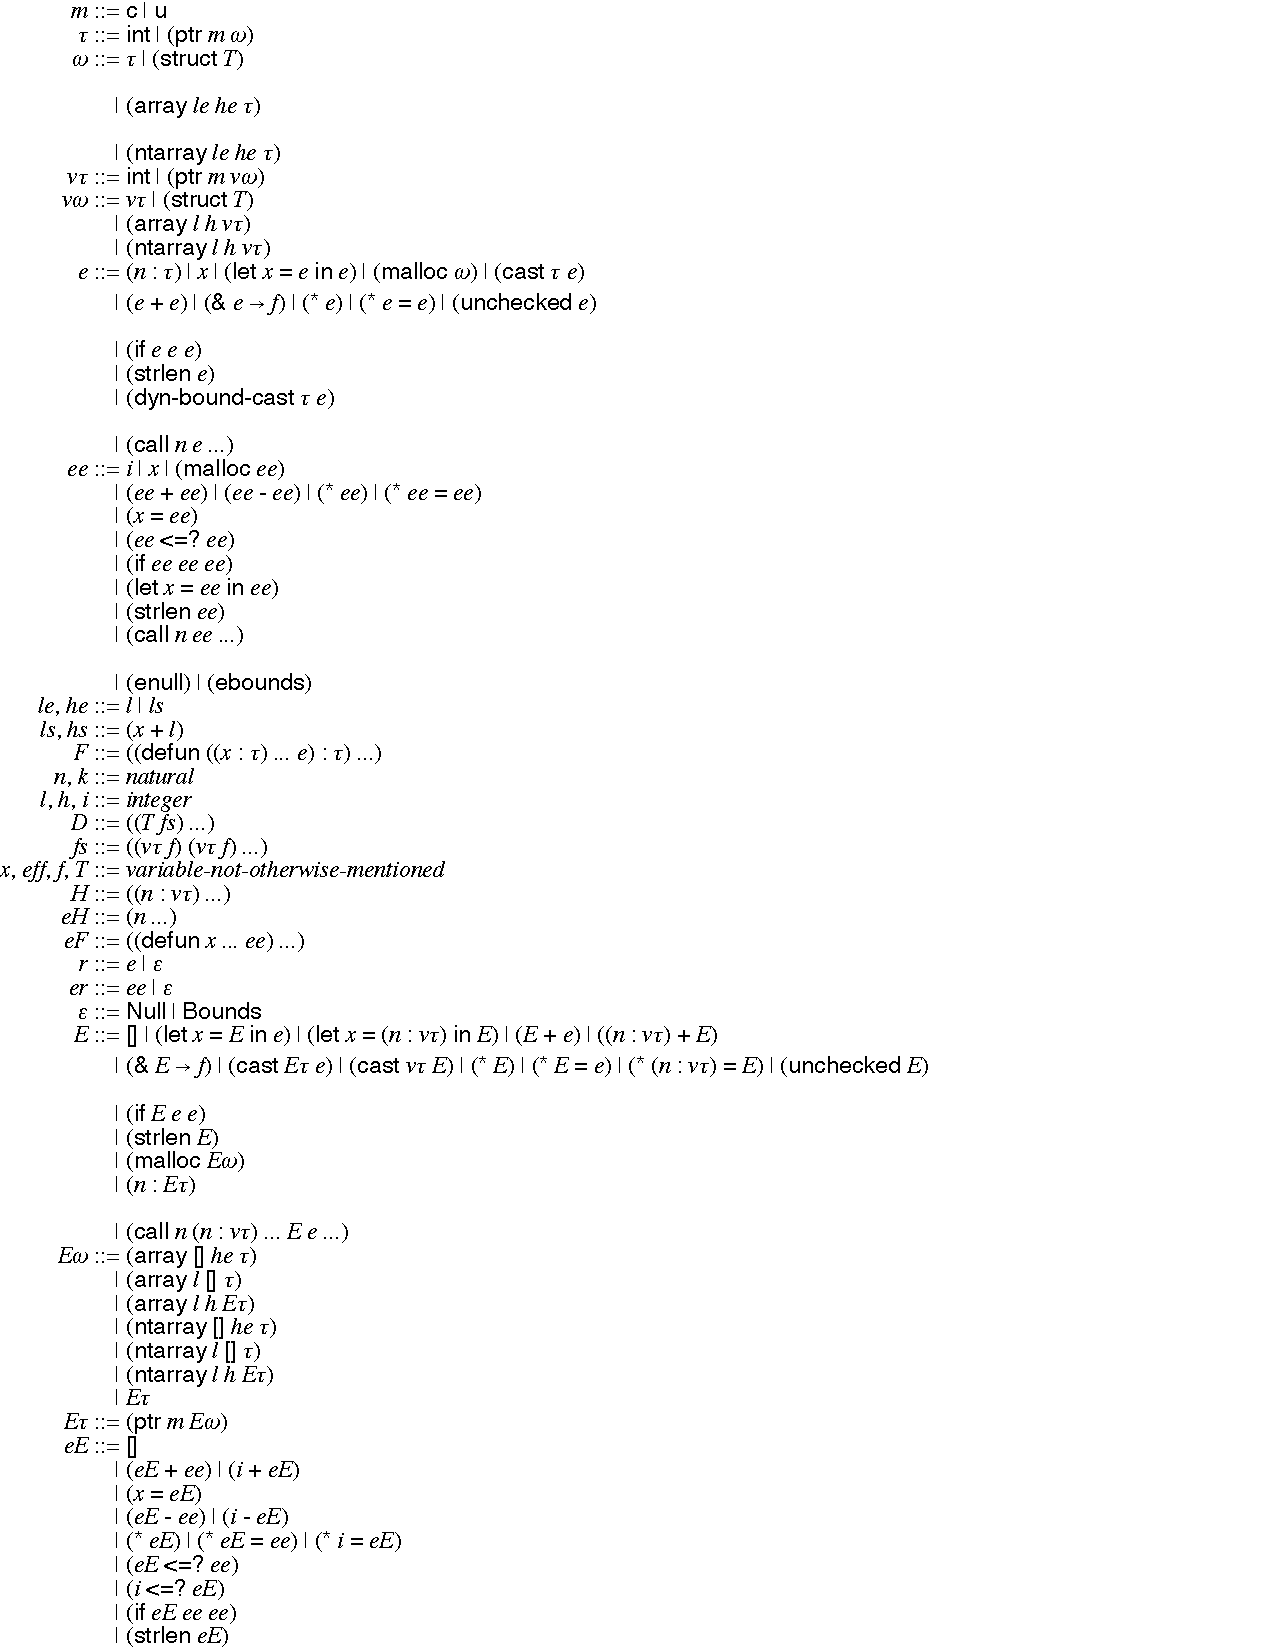
\includegraphics[height=6in]{syntax.pdf}
%   \end{center}
%   \caption{\lang: Syntax}
% \end{figure}

% \begin{figure}
%   \begin{center}
%     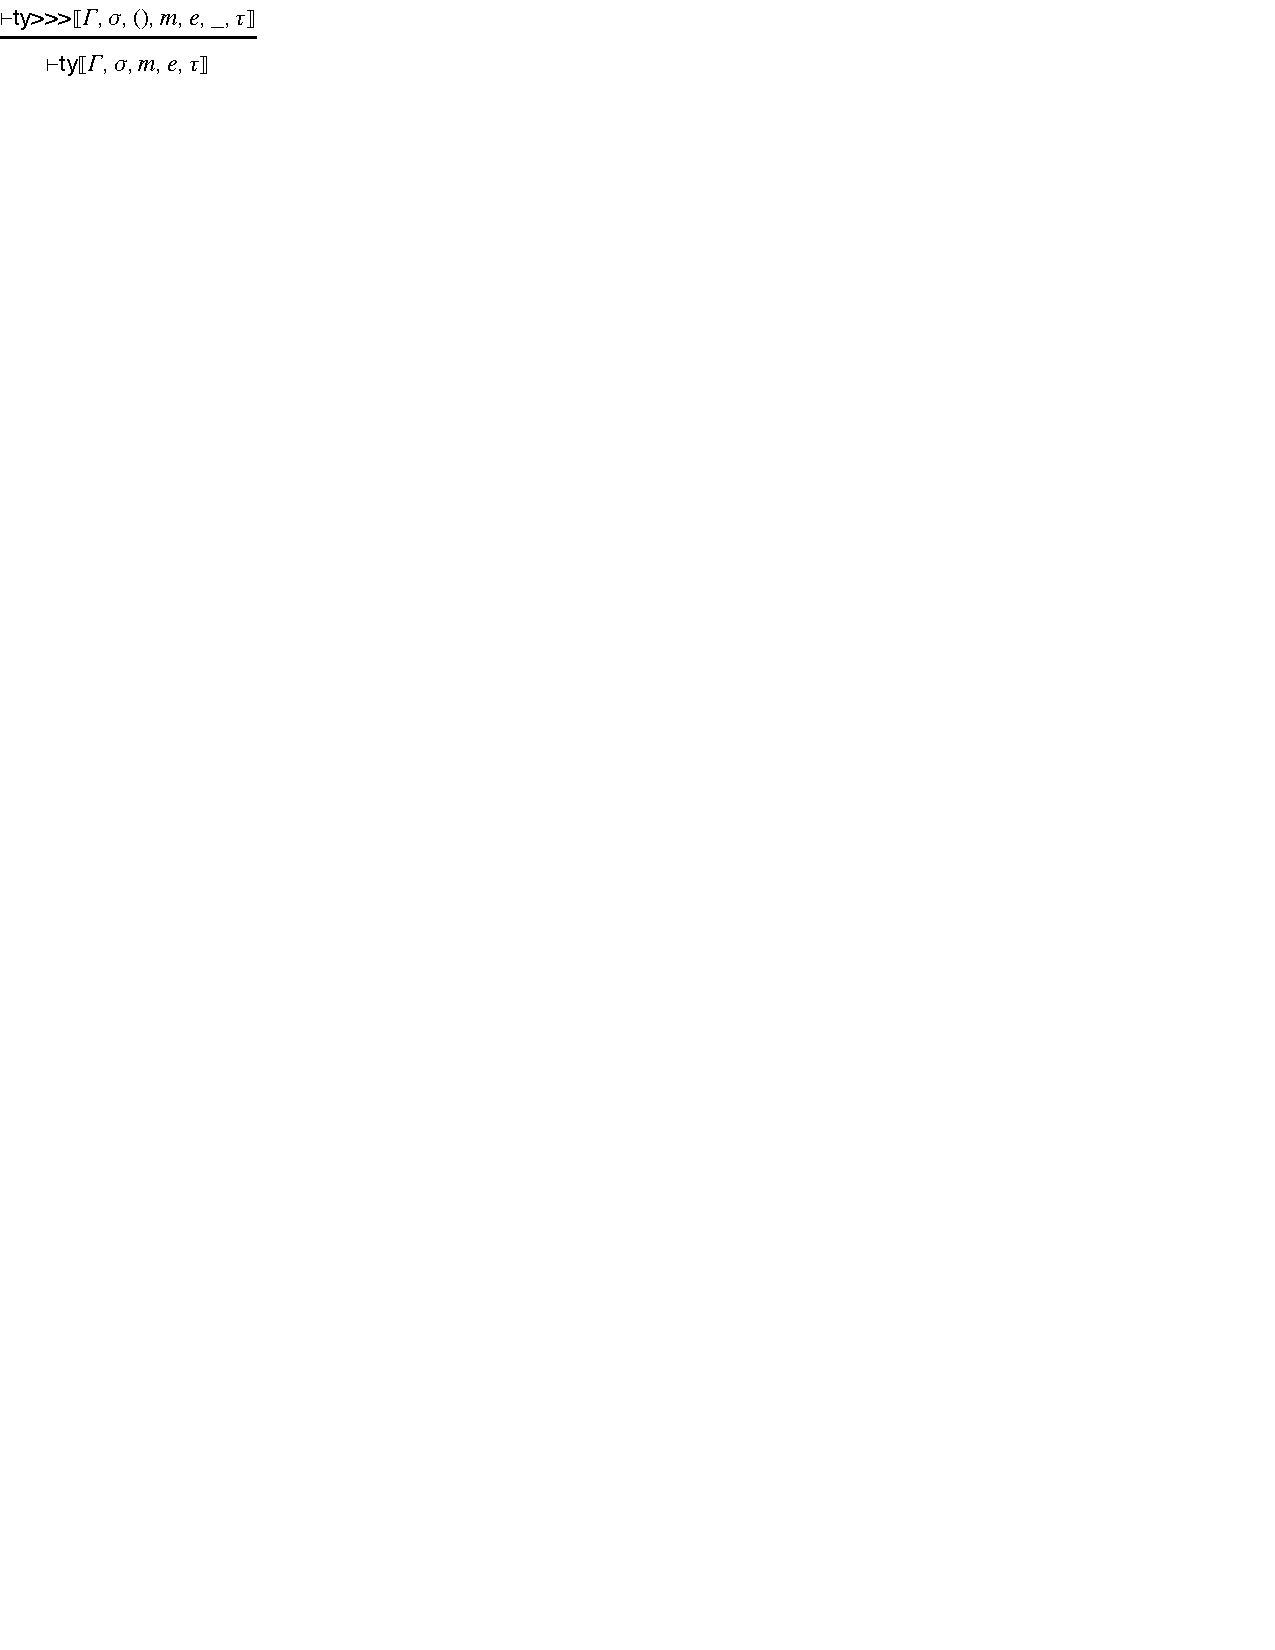
\includegraphics[height=6in]{types.pdf}
%   \end{center}
%   \caption{\lang: Typing}
% \end{figure}
% }
% \liyi{main text begins here. }

% \review{
% While reading the semantics, I found the fact that S-Def and S-DefNull are
%   applicable non-deterministically if n is 0 a bit confusing. Only when
%   reading the meta-theory section I realized that this is not a concrete issue
%   because well-formed heaps are such that $\mathcal{H}(0)$ is never defined. It
%   might be worth pointing this out early on. }
% \mwh{Done.}

\begin{figure}
  \small \centering
  \[ \hspace*{-1.2em}
\begin{array}{l}
\begin{array}{ll}
       \text{Variables:}~ x
& \text{Integers:}~n::=\mathbb{Z} 
\end{array}
\\[0.5em]

\begin{array}{llcllcl}

\text{Context Mode:} & m & ::= & \cmode \mid \umode \\[0.5em]

\text{Pointer Mode:} & \xi & ::= & m \mid \tmode \\[0.5em]

\text{Bound:} & b & ::= & n \mid x \plus n \\
              & \bvar & ::= & (b,b) \\[0.5em]
  
     \text{Word Type:}& \tau &::=& \tint\mid \tptr{\omega}{ \xi}
\\[0.5em]

\text{Type Flag:}&\kappa &::=& nt \mid \cdot
\\[0.5em]

\text{Type:}&\omega &::=& \tau \mid \tallarrayb{\bvar}{\tau} \mid \tfun{\overline{x}}{\overline{\tau}}{\tau}
\\[0.5em]

\text{Expression:}& e & ::= & 
\evalue{n}{\tau} \mid x \mid \ebinop{e}{e}\mid \ecast{\tau}{e} \mid \edyncast{\tau}{e}  \\[0.2em]
&&\mid& \estrlen{x} \mid\estar{e}\mid\eassign{e}{e}  \\[0.2em]
&&\mid& \elet{x}{e}{e} \mid \eif{e}{e}{e}
\\[0.2em]
&&\mid&  \emalloc{\xi}{\omega} \mid \ecall{e}{\overline{e}}
\\[0.2em]
&&\mid&\eunchecked{\overline{x}}{e}
\mid \echecked{\overline{x}}{e}

\end{array}
    \end{array}
  \]
  \caption{\lang Syntax}
  \label{fig:checkc-syn}
\end{figure}

\begin{figure}[t]
{\small
  \begin{mathpar}

  \inferrule[]
  {}
  {m \vdash \tint}

  \inferrule[]
  {\xi \wedge m\vdash \tau \\ \xi \le m}
  {m \vdash \tptr{\tallarrayb{\bvar}{\tau}}{\xi}}

  \inferrule[]
  {\xi \wedge m \vdash \tau\\ \xi \le m}
  {m \vdash \tptr{\tau}{\xi}}

  \inferrule[]
  {\xi \wedge m \vdash \tau\\ \xi \le m \\\\ \fv(\overline{\tau})\cup\fv(\tau)\subseteq \overline{x}}
  {m \vdash \tptr{(\tfun{\overline{x}}{\overline{\tau}}{\tau}}{\xi})}
  \end{mathpar}
}
{\footnotesize
\[
\begin{array}{l} 
\tmode \wedge \cmode = \umode \qquad \xi \wedge \umode = \umode
\qquad \cmode \wedge m = m 
\qquad  m_1 \wedge m_2 = m_2 \wedge m_1
\\[0.2em]
\xi \le \xi \qquad \tmode \le \xi
\end{array}
\\
\]
}
 \caption{Well-formedness for Types}
\label{fig:wftypes}
\end{figure}

%% \dvh{I don't understand the variable grammar.  What is $T$?  What is $\eta$?  I think $\cmode$ and $\umode$ should be in tt font.}
%% \liyi{T and $\eta$ can be moved to the appendix, they are useful only for struct types.}

% \review{
% - Furthermore, inspecting the code also suggests that the expression type (line 155) does not contain constructors for function calls (and I don't see a way to define functions either), conditionals, or strlen, and doesn't distinguish between the two forms of casting. All this contradicts figure 2, and should be clarified
% }
% \liyi{It is in the CheckedC.v file, 392. }
% \mwh{How is this answer helping the reviewer since you've added
%   nothing to the text? Maybe we should add something to an appendix
%   that matches the formalism shown in the paper to definitions in the
%   Coq file?}
% \liyi{The detailed explanation is in the appendix.}

This section describes the formal model of \systemname, called
\lang, making precise its syntax, semantics, and type system. It also
develops \lang's meta-theory, including type soundness, the non-exposure, and the non-crashing
theorem.

\subsection{Syntax}\label{sec:syntax}

The syntax of \lang is given by the expression-based
language presented in Fig.~\ref{fig:checkc-syn}.

There are two notions of type in \lang.  Types $\tau$ classify
word-sized values including integers and pointers, while types
$\omega$ classify multi-word values such as arrays, null-terminated
arrays, functions, and single-word-size values.
%
Pointer types ($\tptr{\omega}{m}$) include a mode annotation ($m$)
which is either checked (\cmode) or unchecked (\umode) and a type
($\omega$) denoting valid values that can be pointed to. Array types include both the type of
elements ($\tau$) and a bound ($\bvar$) comprised of an upper and
lower bound on the size of the array ($(b_l,b_h)$). Bounds $b$ are
limited to integer literals $n$ and expressions $x + n$.
Whether an array pointer is null terminated or not is determined by annotation
$\kappa$, which is $nt$ for null-terminated arrays, and $\cdot$
otherwise (we elide the $\cdot$ when writing the type).
\systemname function types ($\tfun{\overline{x}}{\overline{\tau}}{\tau}$)
reflect its dependent function declrations,
where $\overline{x}$ represents
a list of \tint type variables in a dependent function header,
which bind all bounds appearing in $\overline{\tau}$ and $\tau$.
We have a well-formed requirement for a function type,
such that all variables in $\overline{\tau}$ and $\tau$ are bounded by $\overline{x}$.
Here is the
corresponding \systemname syntax for these types:
\[\hspace*{-0.5em}
\begin{array}{l}
\begin{array}{rcl}
$\code{array_tptr<}$\tau$\code{> : count(}$n$\code{)}$
&\Leftrightarrow& \tarrayptr{0}{n}{\tau}{\tmode}
\\[0.2em]
$\code{nt_array_ptr<}$\tau$\code{> : count(}$n$\code{)}$
&\Leftrightarrow& \tntarrayptr{0}{n}{\tau}{\cmode}
\end{array}
\\[0.2em]
$\code{tptr<(int)(nt_array_tptr<}$\tau$\code{> : count(}$n$\code{),}$\\
\qquad\qquad$\code{nt_array_tptr<}$\tau$\code{>)>: count(}$n$\code{))>}$
\\[0.2em]
\Leftrightarrow\;\; $\tptr{(\tfun{n}{ \tntarrayptr{0}{n}{\tau}{\tmode} \times \tntarrayptr{0}{n}{\tau}{\tmode}}{\tint})}{\tmode}$
\end{array}
\]
As a convention we write $\tptr{\tarrayb{b}{\tau}}{\cmode}$ to mean
$\tptr{\tarray{0}{b}{\tau}}{\cmode}$, so the above examples could
be rewritten $\tptr{\tarrayb{n}{\tau}}{\cmode}$ and
$\tptr{\tntarrayb{n}{\tau}}{\cmode}$, respectively.

\lang expressions include literals ($n\!:\!\tau$), variables ($x$),
 addition ($\ebinop{e_1}{e_2}$), static casts ($\ecast{\tau}{e}$), 
dynamic casts ($\edyncast{\tau}{e}$) \footnote{assumed at compile-time and verified at run-time, see \Cref{app:main}},
the \texttt{strlen} operation ($\estrlen{x}$),
pointer dereference and assignment ($\estar{e}$)
and ($\eassign{e_1}{e_2}$), resp.),
let binding ($\elet{x}{e_1}{e_2}$),
conditionals ($\eif{e}{e_1}{e_2}$),
memory allocation ($\emalloc{\xi}{\omega}$), 
function calls ($\ecall{e}{\overline{e}}$),
unchecked blocks ($\eunchecked{\overline{x}}{e}$), and checked blocks ($\echecked{\overline{x}}{e}$).
% \review{III.A.: the "dynamic cast" terminology may be briefly confused for C++'s
%   RTTI-based dynamic cast feature}
% \mwh{Added reference back to Section 2-B}

Integer literals $n$ are annotated with a type $\tau$ which can be either
$\tint$, or $\tptr{\omega}{m}$ in the case $n$ is being used as 
a heap address (this is useful for the semantics);
$\evalue{0}{\tptr{\omega}{m}}$ (for any $m$ and $\omega$) represents the $\enull$ pointer, as usual. 
The $\texttt{strlen}$ expression operates on variables $x$
rather than arbitrary expressions to simplify managing
bounds information in the type system; the more general case can be
encoded with a \code{let}. We use a less verbose syntax for dynamic bounds
casts; e.g., the following %

\code{dyn_bounds_cast<array_ptr<}$\tau$\code{>>(}$e$\code{, count(}$n$\code{))}

\noindent
becomes $\edyncast{\tptr{\tarrayb{n}{\tau}}{\cmode}}{e}$. 

Compared to the former \checkedc model \cite{li22checkedc},
there are four differences.
First, the \systemname type annotations have well-formed restrictions in \Cref{fig:wftypes}, 
for maintaining non-exposure.
Mainly, in a nested pointer $\tptr{(... \tptr{\tau}{\xi'} ...)}{\xi}$, if the outside mode $\xi$ is 
$\tmode$ or $\umode$, the inside mode $\xi'$ cannot be $\cmode$.
It is worth noting that pointer modes are a three point partial order ($\le$),
where $\tmode$ is the infimum, and
$\xi\wedge m$ is a special meet operation that projects pointer modes onto context modes,
such that a pointer mode $\tmode$ is projected as $\umode$.
Second, $\emalloc{\xi}{\omega}$ includes a mode flag
$\xi$ for allocating different pointers in different heap mode regions.
For simplicity, we disallow $\omega$ to be a function type ($\tfun{\overline{x}}{\overline{\tau}}{\tau}$),
Third, the first expression $e$ in a function call ($\ecall{e}{\overline{e}}$) represents a function pointer.
Fourth, we update $\eunchecked{\overline{x}}{e}$ 
to specify $\overline{x}$ restricting all free variables appearing in $e$.
Additionally, we create $\echeckedtext$ blocks indicating the context mode change from $\umode$ to $\cmode$.
Both the free variables in the $\euncheckedtext$ and $\echeckedtext$ blocks
and the return types cannot be $\cmode$ mode for maintaining non-exposure,
i.e., no checked pointer can be communicated between $\euncheckedtext$ and $\echeckedtext$ blocks.

\lang aims to be simple enough to work with, but powerful enough to
encode realistic \systemname idioms. For example, mutable local
variables can be encoded as immutable locals that point to the heap;
the use of \code{&} can be simulated with \code{malloc};
and loops can be encoded as recursive function calls. \code{struct}s are
not in Fig.~\ref{fig:checkc-syn} for space reasons, but they are
actually in our model, and developed in
\iftr
Appendix~\ref{appx:struct}.
\else
the supplemental report~\cite{checkedc-tech-report}.
\fi
C-style \code{union}s have no safe typing
in \checkedc, so we omit them.
Additional syntactic descrition is listed in the \checkedc formalism paper \cite{li22checkedc}.


% \mwh{NOTE: COULD WORK THE FOLLOWING INTO THE ABOVE DESCRIPTION OF
%   POINTERS: Array and NT-array types have two relative bounds, whose structures
% can be either an integer or a variable plus an integer. For example,
% if we have the expression
% $x\texttt{=}\emalloc{\tarrayb{(0,10)}{\tint}}$, $x$ then has the type
% $\tptr{\tarrayb{10}{\tint}}{\cmode}$, which represents an array
% pointer of size $10$. The bounds ($(b_l,b_h)$ in
% $\evalue{p}{\tptr{\tarrayb{(b_l,b_h)}{\tau}}{m}}$) indicate relative
% offsets from this pointer of the accessible memory, i.e., $p+b_l$ and
% $p+b_h$. As such, a pointer can only be directly dereferenced if 0 is
% included within the annotated range.  If following the $\emalloctext$
% operation, we execute $*(x-1)$ and $*(x\plus 10)$. The two expressions
% are not valid, because the type of the two expressions $(x-1)$ and
% $(x\plus 10)$ are $\tarrayptr{1}{11}{\tint}{\cmode}$ and
% $\tarrayptr{-10}{0}{\tint}{\cmode}$ and $0$ in these two cases are not
% in the ranges: $[1,11)$ and $[-10,0)$. Thus, in order for a $\cmode$
% pointer with type $\tarrayptr{b_l}{b_h}{\tint}{\cmode}$ to be
% accessible in \checkedc, $0$ must be in the range of $[b_l,b_h)$.}

\begin{figure}
{\small
$\hspace*{-1.2em}
    \begin{array}{l}
    \begin{array}{lll}
\mu & ::= & \evalue{n}{\tau}\\
e & ::= & \ldots \mid \ret{x}{\mu}{e}\\
r & ::= & e \mid \enull \mid \ebounds\\
E &::=& \Box \mid \ebinop{E}{e} \mid \ebinop{\evalue{n}{\tau}}{E}\mid \ecast{\tau}{E} \mid \edyncast{\tau}{E} \mid\estar{E}\mid\eassign{E}{e}\\[0.2em]
&&\mid\eassign{\evalue{n}{\tau}}{E}\mid \elet{x}{E}{e}\mid \eif{E}{e}{e}\\[0.2em]
&&\mid \ecall{E}{\overline{e}} \mid \ecall{\evalue{n}{\tau}}{\overline{E}} \mid 
\eunchecked{\overline{x}}{E}
\mid \echecked{\overline{x}}{E}


\end{array}
\\ \\
    \end{array} 
$
  \begin{mathpar}
    \inferrule{ m=\mode(E) \\
      e=E[e'] \\
      (\varphi,\heap,e') \longrightarrow (\varphi',\heap',e'')}
    {(\varphi,\heap,e)\longrightarrow_{m} (\varphi',\heap',E[e''])}

    \inferrule{ \umode=\mode(E) \\
      e=E[e'] \\
      \tau=\type(e')}
    {(\varphi,\heap,e)\longrightarrow_{\umode} (\varphi,\heap,E[\evalue{0}{\tau}])}

  \end{mathpar}
}
{\footnotesize
\[
\begin{array}{l} 
\mode(E)=\mode'(E,\cmode)
\\[0.2em]
\mode'(\Box,m)=m
\\[0.2em]
\mode'(\eunchecked{\overline{x}}{E},m)=\mode'(E,\umode)
\\[0.2em]
\mode'(\echecked{\overline{x}}{E},m)=\mode'(E,\cmode)
\\[0.2em]
\mode'(\alpha({E}),m)=\mode'(E,m)\;\;{[\emph{owise}]}
\end{array}
\\
\]
}
  \caption{\lang Semantics: Evaluation}
  \label{fig:c-context}
\end{figure}

\subsection{Semantics}\label{sec:semantics}

% The semantics
% gives an independent account of spatial safety in \lang by
% checking pointer bounds based on the annotations carried on types at
% run-time.  While this account makes clear that bounds checking occurs
% as expected, it suggests an implementation that uses fat pointers to
% carry bounds.  We resolve this tension in the subsequent section on
% compilation and show that an implementation faithful to the semantics
% can be obtained without fat pointers.  
% \review{repeat that the stack is immutable at this point?}
% \liyi{Is it? Is the stack immutable? What does the immutable mean? 
%   In a stack, the variable values can be changed? Right?
%   The pointer address itself cannot be changed once it is created, but the stack variable content can be updated?  }
% \mwh{It certainly seems to be immutable: Your create stack frames
%   using let binding, and the let-bound variables will always be bound
%   to the same things. I.e., stack cells are immutable.}

% \review{this raises a fair amount of questions regarding the treatment of the
%   NULL pointer at this stage of the paper... is it modeled as 0, as returned by
%   `malloc`? are dynamic checks inserted by CheckedC to guarantee that no NULL
%   pointer is dereferenced?}
% \mwh{Yes, it is modeled as 0, and the semantics checks for
%   dereferences of 0. }

The operational semantics for \lang is defined as a small-step
transition relation with the judgment $ (\varphi,\heap,e)
\longrightarrow_m (\varphi',\heap',r)$. Here, $\varphi$ is a
\emph{stack} mapping from variables to values $\evalue{n}{\tau}$ and
$\heap$ is a \emph{heap} that is partitioned into two parts ($\cmode$ and $\umode$ regions), each of which
maps addresses (integer literals) to values $\evalue{n}{\tau}$.
If a pointer has mode $\cmode$, it lives in the $\cmode$ region; otherwise, it lives in the $\umode$ region.
We wrote $\heap(m,n)$ to retrieve the $n$-location heap value in the $m$ region,
and $\heap(m)[n\mapsto \mu]$ to update location $n$ with the value $\mu$.
It is worth noting that \systemname is not a fat-pointer system;
thus, in every heap update, the value type annotation remains the same through program executions.
Additionally, for both stack and heap, 
we ensure $\fv(\tau)=\emptyset$ for all the value type annotations $\tau$.

While heap bindings can change, stack bindings are immutable---once
variable $x$ is bound to $\evalue{n}{\tau}$ in $\varphi$, that binding will not
be updated; we can model mutable stack variables as pointers into the
mutable heap.
As mentioned, value $\evalue{0}{\tau}$
represents a $\enull$ pointer when $\tau$ is a pointer type;
correspondingly, $\heap(m,0)$ should always be undefined.
The relation steps to a \emph{result} $r$,
which is either an expression or a $\enull$ or $\ebounds$ failure,
representing a null-pointer dereference or out-of-bounds access,
respectively. Such failures are a \emph{good} outcome; stuck states
(non-value expressions that cannot transition to a result $r$)
characterize undefined behavior.
%
The context mode $m$ indicates whether the
stepped redex within $e$ was in a checked ($\cmode$) or
unchecked ($\umode$) region.

The rules for the main operational semantics
judgment---\emph{evaluation}---are given at the bottom of
Fig.~\ref{fig:c-context}.
The first rule takes an expression $e$, decomposes
it into an \emph{evaluation context} $E$ and a sub-expression $e'$
(such that replacing the hole $\Box$ in $E$ with $e'$ would yield
$e$), and then evaluates $e'$ according to the \emph{computation}
  relation $(\varphi,\heap,e') \longrightarrow (\varphi,\heap,e'')$,
whose rules are given in Fig.~\ref{fig:semantics}, discussed
shortly. 
The second rule describes the exception handling 
for possible crashing behaviors in unchecked region.
A program in $\umode$ mode can non-deterministically crash
and the \systemname sandbox mechanism recorvers
the program to a safe point ($\evalue{0}{\tau}$)
and continues with the existing program state.
There are other rules for describing the halts of evaluation to $\enull$ and $\ebounds$ states in \Cref{app:main}.

%\footnote{This approach is that of the PLT Redex model of \lang; the Coq
%development uses a slightly simpler syntax to achieve the same
%effect.}
% \review{the special case raises questions, e.g. why is this syntax-driven and
%   not type-driven? }
% \liyi{This describes the semantic transition rules. We are using context evaluation framework to define the transition rules as the $E$ definition in Fig.3. like $\frac{x \Rightarrow y}{x+z \Rightarrow y + z}$, I don't know how type-driven can help us define translation rules.  }
% \mwh{Don't follow the above. I don't see this ``context transition
%   rule'' anywhere, and I'm not sure how it would fire, if we had it.}
% \liyi{The comment seems to confuse the meaning of the text about the if-then-else rules. Making the rule specific will help. }
The $\mode$ function
determines the context mode when evaluating $e'$ based on the context $E$.
For any program execution, the top context mode always starts with $\cmode$ ($\mode(E)=\mode'(E,\cmode)$).
The result context mode is depeneded on where $\Box$ locates.
If it occurs within $(\eunchecked{\overline{x}}{E'})$ inside $E$ without
a surrounding $\echeckedtext$ block, then the mode is
$\umode$; if the exact opposite happens (within $(\echecked{\overline{x}}{E'})$ without surrounding $\euncheckedtext$ blocks),
the mode is $\cmode$; the other cases ($\mode'(\alpha({E}),m)=\mode'(E,m)$) are recursively defined by the above base cases ($\alpha$ represents any syntactic categories in \Cref{fig:c-context} other than $\Box$, $\euncheckedtext$, and $\echeckedtext$).
Evaluation contexts $E$ define a standard left-to-right evaluation order. (We explain the
$\ret{x}{\mu}{e}$ syntax shortly.)
% For a term $e$, $C$ is a context if any
% only if it contains a $\Box$ hole term in one of the subterm position
% in $e$. $\Box$ indicates the break point where we split $e$ into $C$
% and a subterm $e'$ such that $C[e'] = e$.  For a function call
% $\ecall{f}{\overline{e}}$, a valid context ($\overline{C}$) is defined
% as any one of the elements in the list $\overline{e}$ being a
% context. We show a rule of the upper level \checkedc semantics. The
% rule splits a term $e$ into a context $C$ and redex $e'$.  If subterm
% $e'$ is transitioned to $e_a$, $C[e']$ is transitioned to
% $C[e_a]$.

\begin{DIFnomarkup}
\begin{figure*}[t]
{\small
  \begin{mathpar}
        \inferrule[S-DefC]{\heap(\cmode,n)=\evalue{n_a}{\tau_a} }
    {(\varphi,\heap,\estar{\evalue{n}{\tptr{\tau}{c}}}) \longrightarrow (\varphi,\heap,\evalue{n_a}{\tau})}

    \inferrule[S-AssignArrC]{\heap(\cmode,n)=\evalue{n_a}{\tau_a}\\ 0 \in [n_l,n_h) }
      {(\varphi,\heap,\eassign{\evalue{n}{\tallarrayptr{n_l}{n_h}{\tau}{\cmode}}}{\evalue{n_1}{\tau_1}}) \longrightarrow (\varphi,(\heap,\cmode)[n \mapsto \evalue{n_1}{\tau_a}],\evalue{n_1}{\tau})}

        \inferrule[S-DefT]{\heap(\umode,n)=\evalue{n_a}{\tau_a}
         \\  \emptyset;\heap ; \emptyset \vdash_{\umode}\evalue{n_a}{\tau} }
    {(\varphi,\heap,\estar{\evalue{n}{\tptr{\tau}{\tmode}}}) \longrightarrow (\varphi,\heap,\evalue{n_a}{\tau})}

    \inferrule[S-AssignArrT]{\heap(\umode,n)=\evalue{n_a}{\tau_a}\\ 0 \in [n_l,n_h)
               \\  \emptyset;\heap ; \emptyset \vdash_{\umode}\evalue{n_1}{\tau} }
      {(\varphi,\heap,\eassign{\evalue{n}{\tallarrayptr{n_l}{n_h}{\tau}{\tmode}}}{\evalue{n_1}{\tau_1}}) \longrightarrow (\varphi,(\heap,\umode)[n \mapsto \evalue{n_1}{\tau_a}],\evalue{n_1}{\tau})}

    \inferrule[S-DefNull]{}{(\varphi,\heap,\estar{\evalue{0}{\tptr{\omega}{\cmode}}}) \longrightarrow (\varphi,\heap,\enull)}

    \inferrule[S-Cast]
              {}
              {(\varphi,\heap,\ecast{\tau}{\evalue{n}{\tau'}}) \longrightarrow (\varphi,\heap,\evalue{n}{\varphi(\tau)})}

    \inferrule[S-RetEnd]{}{(\varphi,\heap,\ret{x}{\mu}{\mu'}) \longrightarrow (\varphi,\heap,\mu')}

        \inferrule[S-Let]{}{(\varphi,\heap,\elet{x}{\evalue{n}{\tau}}{e}) \longrightarrow (\varphi,\heap,\ret{x}{\evalue{n}{\tau}}{e})}

    \inferrule[S-RetCon]{\varphi(x)=\mu\\ (\varphi[x\mapsto \mu'],\heap,e) \longrightarrow (\varphi',\heap',e')}{(\varphi,\heap,\ret{x}{\mu'}{e}) \longrightarrow (\varphi'[x\mapsto \mu],\heap',\ret{x}{\varphi'(x)}{e'})}

    \inferrule[S-Unchecked]{}{(\varphi,\heap,\eunchecked{\overline{x}}{\mu}) \longrightarrow (\varphi,\heap,\mu)}

    \inferrule[S-FunC]{ \Xi(\cmode,n) = \tau\;(\evalue{\overline{x}}{\overline{\tau}})\;(\cmode,e)}
        {(\varphi,\heap,\ecall{\evalue{n}{(\tptr{\tau}{\cmode})}}{{\evalue{\overline{n_a}}{\overline{\tau_a}}}}) \longrightarrow
   (\varphi,\heap, \mathtt{let}\;\overline{x}={\evalue{\overline{n}}{(\overline{\tau}[\overline{n} / \overline{x}])}}\;\mathtt{in}\;\ecast{\tau[\overline{n} / \overline{x}]}{e})}

    \inferrule[S-Checked]{}{(\varphi,\heap,\echecked{\overline{x}}{\mu}) \longrightarrow (\varphi,\heap,\mu)}

    \inferrule[S-FunT]{ \Xi(\umode,n) = \tau\;(\evalue{\overline{x}}{\overline{\tau}})\;(\tmode,e)
                  \\ \emptyset;\heap ; \emptyset \vdash_{\umode}\evalue{n}{\tptr{\tau}{\tmode}}}
        {(\varphi,\heap,\ecall{\evalue{n}{(\tptr{\tau}{\tmode})}}{{\evalue{\overline{n_a}}{\overline{\tau_a}}}}) \longrightarrow
   (\varphi,\heap, \mathtt{let}\;\overline{x}={\evalue{\overline{n}}{(\overline{\tau}[\overline{n} / \overline{x}])}}\;\mathtt{in}\;\ecast{\tau[\overline{n} / \overline{x}]}{e})}


 % \inferrule[S-IfNTNot]{\varphi(x)=\evalue{n}{\tntarrayptr{n_l}{n_h}{\tau}{\cmode}} \\ \heap(n)\neq 0\\ 0 < n_h}
 %            {(\varphi,\heap,\eif{\estar{x}}{e_1}{e_2}) \longrightarrow (\varphi,\heap,e_1)}

\end{mathpar}
}
% {\footnotesize
% \begin{center}
% $
% \begin{array}{l}
% \tau[\overline{n} / \overline{x}]\texttt{(with types }\evalue{\overline{x}}{\overline{\tau}}\texttt{)}\triangleq \forall n_i\in\overline{n}\;x_i\in\overline{x}\;\tau_i\in\overline{\tau}\;.\;\tau_i = \tint \Rightarrow \tau[n_i / x_i]\\[0.2em]
% \mathtt{let}\;\overline{x}=\overline{e}\;\mathtt{in}...\triangleq \mathtt{let}\;x_0=e_0\;\mathtt{in}\;\mathtt{let}\;x_1=e_1\;\mathtt{in}...
% \end{array}
% $
% \end{center}
% }
\caption{\lang Semantics: Computation (Selected Rules)}
\label{fig:semantics}
\end{figure*}
\end{DIFnomarkup}

\begin{figure}[t]
{\small
{\captionsetup[lstlisting]{margin = 8 mm}
  \begin{lstlisting}[xleftmargin=8 mm]
nt_array_ptr<char> safe_strcat
   (nt_array_ptr<char> dst : count(n),
    nt_array_ptr<char> src : count(0), int n) {
  int x = strlen(dst);
  int y = strlen(src);
  nt_array_ptr<char> c : count(n) =
    dyn_bounds_cast
           <nt_array_ptr<char>>(dst,count(n));
    // sets c == dst with bound n (not x)
  if (x+y < n) {
    for (int i = 0; i < y; ++i)
      *(c+x+i) = *(src+i);
    *(c+x+y) = '\0';
    return dst;
  }
  return null;
}
  \end{lstlisting}
}
}
\caption{Implementation of safe \code{strcat}}
\label{fig:strcat-ex}
\end{figure}

% \review{Fig4: it was hard to tell which cases were stuck states, or could reduce
%   owing to a rule that was not shown}
% \mwh{Stuck states are those where the expression is a non-value and
%   not $\enull$ or $\ebounds$. Updated III-B and III-D.}
% \review{Fig4: can the rules be presented in the same order they were introduced in
%   the paper?}
% \liyi{ Reordered }

% \review{Fig4: S-FUN: $\vec\tau_a$ seems unused; why?}
% \liyi{the list of $\tau_a$ is a list of input argument types. These
%   are used during type checking, but not during evaluation (as is
%   typical).} 

% LEO: This has an overfull line...?

Fig.~\ref{fig:semantics} shows selected rules for the computation
relation; we explain them with the help of the example in \Cref{fig:checkedc-example-1} and \Cref{fig:checkedc-example-2}.

\ignore{
 in
Fig.~\ref{fig:strcat-ex},
  which defines a 
  safe version of \code{strcat} (using actual Checked C syntax).  The
  function takes a target 
  pointer \code{dst} of capacity \code{n}, where the first null
  character (determined by \code{strlen}) is at index \code{x} where
  $0 \leq $\code{x}$ \leq n$. It concatenates the \code{src} buffer to
  the end of \code{dst} as long as \code{dst} has sufficient space.}

% Below, we introduce low-level transition semantics for some case operations. The design of the low-level individual operation semantics is carefully engineered to perform match our compiler's behavior, such as correctly characterizing the bound widening behaviors for NT-array pointers, even though it is written in terms of fat-pointer formalization.

\myparagraph{Checked and Tainted Pointer Operations}
%
The rules for pointer related operations---\textsc{S-DefC},
\textsc{S-DefT}, \textsc{S-AssignArrC}, \textsc{S-AssignArrT},
\textsc{S-DefNull}, and \textsc{S-Cast}.
The first five are deference and assignment operations---illustrate how the semantics checks bounds.
Rule \textsc{S-DefNull} transitions attempted null-pointer
dereferences to $\enull$, whereas \textsc{S-DefC} dereferences a \cmode-mode
non-null (single) pointer.
When $\enull$ is returned by the
computation relation, the evaluation relation halts the entire
evaluation with $\enull$ (using a rule not shown in Fig.~\ref{fig:c-context}); it
does likewise when $\ebounds$ is returned (see \Cref{sec:rem-semantics}).
\textsc{S-AssignArrC} assigns to an array as long as 0 (the point of
dereference) is within the bounds designated by the pointer's annotation
and strictly less than the upper bound. 

\textsc{S-DefT} and \textsc{S-AssignArrT} are similar rules to \textsc{S-DefC} and \textsc{S-AssignArrC} for tainted pointers.
Any dynamic heap use of a tainted pointer requires a verification.
Performing such a verification equates to performing a type check for a pointer constant in \Cref{fig:const-type}.
We explain this shortly in \Cref{sec:type-system}.
For now, the verification step, e.g. $\umode;\emptyset;\heap ; \emptyset \vdash\evalue{n_a}{\tau}$ in \textsc{S-DefC},
means we verify that the value $n_a$ has type $\tau$ in the $\umode$ region heap.

Static casts of a literal $n\!:\!\tau'$ to a type $\tau$ are handled
by \textsc{S-Cast}. In a type-correct program, such casts are
confirmed safe by the type system no matter
if the target is a $\tmode$ or $\cmode$ pointer. To evaluate a cast, the rule
updates the type annotation on $n$. Before doing so, it must
``evaluate'' any variables that occur in $\tau$ according to their
bindings in $\varphi$. For example, if $\tau$ was
$\tarrayptr{0}{x+3}{\tint}{\cmode}$, then $\varphi(\tau)$ would
produce $\tarrayptr{0}{5}{\tint}{\cmode}$ if $\varphi(x) = 2$.
The full formalism, including \kw{struct}
and null-terminated bound widening pointer operations, is given in \Cref{app:main}.

% \review{- on page 6, section IIIC, paragraph "Pointer Access" mentions that checked pointers cannot be dereferenced in unchecked blocks - this looks funny, shouldn't it be the other way around? The Coq code contains the hypothesis m'=Unchecked -> m Unchecked in various rules of definition well-typed (BoundCheckedC, line 669; rule TyDeref in the code seems closest to the figure's T-DefArr and T-Def in the appendix, although it's a bit concerning that there's no 1-to-1 correspondence of the rules in the code and the paper).
% }
% \liyi{Yeah. It is another typo. It should be the other way around.  }

\myparagraph{Unchecked and Checked Blocks}
%
Semantically, $\euncheckedtext$ and $\echeckedtext$ blocks 
(\textsc{S-Unchecked} and \textsc{S-Checked}) act as a classical C block structures.
The interesting part is their type rules in \Cref{sec:type-system}.

\myparagraph{Binding and Function Calls}
%
The semantics handles variable scopes using the special $\erettext$
form. \textsc{S-Let} evaluates to a configuration whose stack
is $\varphi$ extended with a binding for $x$, and whose expression is
$\ret{x}{\evalue{n}{\tau}}{e})$ which keeps $\varphi$ unchanged, but
remember $x$ with the new value $\evalue{n}{\tau}$ in the scope $e$.
Every time when Evaluation proceeds on $e$ (Rule \textsc{S-RetCon}),
we install the current stack value $\evalue{n}{\tau}$ for $x$ in $\varphi$,
after one-step evaluation is completed, we restore the result $\varphi'(x)$ 
in the result $\ret{x}{\varphi'(x)}{e'})$.
This procedure continues until it becomes a literal
$n\!:\!\tau$, in which case \textsc{S-RetEnd} remove the $\kw{ret}$ frame and evaluates to
$n\!:\!\tau$. 

Function calls are handled by \textsc{S-FunC} and \textsc{S-FunT},
for \cmode and \tmode mode function pointers, respectively. 
A call to function $f$ causes $f$'s
definition to be retrieved from $\Xi$,
% LEO: This is the first occurence of \Xi. It is explained,
% but reads a bit awkward as it's unclear this is its "introduction"
which maps function names to
function data $\tau\;(\evalue{\overline{x}}{\overline{\tau}})\;(\xi,e)$, where
$\tau$ is the return type, $(\evalue{\overline{x}}{\overline{\tau}})$
is the parameter list of variables and their types, 
$\xi$ determines the mode of the function, and $e$ is the
function body. 
Similar to \heap, the global function store $\Xi$ is also partitioned into
two parts ($\cmode$ and $\umode$ regions), each of which
maps addresses (integer literals) to the function data described above.

The \systemname functions are dependent functions.
Recall that array
bounds in types may refer to in-scope variables; e.g., parameter
\code{dst}'s bound \code{count(n)} refers to parameter \code{n} on lines
2-3 in Fig.~\ref{fig:strcat-ex}. 
%All dependent bound variables appearing in function headers 
%are bounded by a variable list in the function pointer type, which is checked in the type rule.
Semantically,
the call is expanded into a \texttt{let} which binds
parameter variables $\overline{x}$ to the actual arguments
$\overline{n}$, but annotated with the parameter types
$\overline{\tau}$ (this will be safe for type-correct programs). The
function body $e$ is wrapped in a static cast
$(\tau[\overline{n} / \overline{x}])$ which is the function's return
type but with any parameter variables $\overline{x}$ appearing in that
type substituted with the call's actual arguments $\overline{n}$. To
see why this is needed, suppose that \code{safe_strcat} in
Fig.~\ref{fig:strcat-ex} is defined to return a
\code{nt_array_ptr<int>:count(n)} typed term, and assume that we
perform a \code{safe_strcat} function call as
\code{x=safe_strcat(a,b,10)}. After the evaluation of \code{safe_strcat}, the
function returns a value with type \code{nt_array_ptr<int>:count(10)}
because we substitute bound variable \code{n} in the 
defined return type with \code{10} from the function call's
argument list.
Note that the \textsc{S-FunC} and \textsc{S-FunT} rules replace the
  annotations $\overline{\tau_a}$ with
  $\overline{\tau}$ (after instantiation) from the function's
  signature. Using $\overline{\tau_a}$ when executing the body of
the function has no impact on the soundness of \lang, but will violate
Theorem~\ref{simulation-thm}, which we introduce in Sec.~\ref{sec:compilation}.

 %  For this rule and
% \textsc{S-StrWiden}, this widening persists in the current stack
% frame. When $x$ goes out of scope, .

% \textsc{S-IfNTF} does not widen when seeing null; rule
% \textsc{S-IfNTNot} sees a non-null character, but the pointer is not
% at its upper bound, so the bounds cannot be widened. 

% \ignore{
% Fig.~\ref{fig:semantics} provides the low-level semantic rules for operations involving NT-array pointers, mainly, the $\estrlentext$ and $\eiftext$ operations. The semantics has concurred the ambiguity in the \checkedc specification, e.g., we define the exact behavior of the $\estrlentext$ operation to return the length between the current pointer position and the first null-character.
% We also utilize new technique in our compiler so that the scope of the bound widening behavior in our formalization is a little longer. More details are in Sec.~\ref{sec:compilation}.

% The first rule defines the evaluation behavior of a $\estrlentext$ operation. Given a pointer $x$ with its type $\tntarrayptr{0}{n_h}{\tau}{m}$, the application of such operation takes the address of the pointer $x$, and search incrementally the heap positions next to the address $x$ until we find a $0$ value (representing a null character). We return the value $n_a$ as the length, and update the bound information in the stack for $x$. In the compilation, we use a ghost variable to record such bound changes without using fat-pointer implementations.

% The last three rules in Fig.~\ref{fig:semantics} describe the semantic behaviors of an $\eiftext$ branching operation when the Boolean guard is a dereference of an NT-array pointer. The first one states that if the type upper bound of the pointer $x$ is $0$, and the pointer data value $n_a$ is not $0$, we can conclude that the upper bound is not the last position of the NT-array pointer, so we can then update $1$ in the upper bound while jump to the $\etrue$ branch. The second rule describes that we do not extend the upper bound if the upper-bound of the type of $x$ is not zero because we know that we are not in the NT-array's last position. The third rule describes the behavior of jumping to the $\efalse$ branch when the pointer content is $0$. In this case, we also do not need to increase the upper-bound of the type of $x$.}

\subsection{Typing}\label{sec:type-system}

%% DVH: covered above.
%% Any \checkedc expression is a word type object ($\tau$ in Fig.~\ref{fig:checkc-syn}), which is either an \tint{} or a pointer. A pointer can be either a word type $\tau$, an array $\tarray{b}{b}{\tau}$, or an NT-array $\tntarray{b}{b}{\tau}$. Each pointer type is associated with a mode $m$ indicating whether the pointer is checked (\cmode) or unchecked ($\umode$).

We now turn to the \lang type system.
% The design of the type
% system has been carefully constructed to ensure the expected
% properties of progress and preservation, but also so that the
% type-based compilation strategy detailed later is correct and
% economical in its representation of pointers.
%
The typing judgment has the form $\Gamma;\Theta\vdash_m e : \tau$,
which states that in a type environment $\Gamma$ (mapping variables to
their types) and a predicate environment $\Theta$ (mapping integer-typed
variables to Boolean predicates), expression $e$ will have type $\tau$ if evaluated
in mode $m$. Key rules for this judgment are given in
Fig.~\ref{fig:type-system-1}.
% \review{text says $u < c$ but this seems to contradict the paragraph right
%   after, because if $m = u$ then $u <= c$ and it seems like T-DefArr *does*
%   allow me to dereference a checked pointer in unchecked mode...? Or am I
%   missing something?}
% \liyi{ Why it will be a problem in dereferencing a checked pointer in unchecked mode?
%    unchecked regions contain history C code that is not translated to Checked-C syntax, but it could also mean that the translation is under construction, so that we are free to put checked-C code there, and we gaurantee that the checked-pointers in unchecked-mode are also spatially safe. The opposite is not true, where you cannot use (dereference/assign) a unchecked-pointer in a checked mode. }
All remaining rules
are given in
\iftr
Appendix~\ref{sec:literal-pointer-typing}~and~\ref{rem-type}.
\else
the supplemental report~\cite{checkedc-tech-report}.
\fi

\begin{DIFnomarkup}
\begin{figure*}[t]
{\small
  \begin{mathpar}
   \inferrule[T-ConstU]
       { \neg \cmode(\tau)}
       {\Gamma;\Theta\vdash_u \evalue{n}{\tau} : \tau}

   \inferrule[T-ConstC]
       {\Theta;\heap;\emptyset \vdash_c n : \tau}
       {\Gamma;\Theta\vdash_c \evalue{n}{\tau} : \tau}

    \inferrule[T-Def]
              {\xi \leq m \\\\\Gamma;\Theta \vdash_m e : \tptr{\tau}{\xi}}
              {\Gamma;\Theta \vdash_m \estar{e} : \tau}

    \inferrule[T-AssignArr]
              {\Gamma; \Theta \vdash_m e_1 : \tptr{\tallarrayb{\bvar}{\tau}}{\xi}\\\\
                \Gamma; \Theta \vdash_m e_2 : \tau' \\\\
                \tau'\sqsubseteq_{\Theta} \tau\\
                \xi \leq m}
              {\Gamma; \Theta \vdash_m \eassign{e_1}{e_2} : \tau}              

     \inferrule[T-CastPtr]
               {\Gamma;\Theta \vdash_m e : \tau' \\
                 \tau' \sqsubseteq \tptr{\tau}{\xi}}
               {\Gamma;\Theta \vdash_m \ecast{\tptr{\tau}{\xi}}{e} : \tptr{\tau}{\xi}}
                
   \inferrule[T-Let]
    { x\not\in \fv(\tau') \\
        \Gamma;\Theta \vdash_m e_1 : \tau \\\\
          \Gamma[x\mapsto \tau];\Theta \vdash_m e_2 : \tau'
             }
    {\Gamma;\Theta \vdash_m \elet{x}{e_1}{e_2} : \tau'}

   \inferrule[T-LetInt]
    { x\in \fv(\tau') \Rightarrow e_1 \in \text{Bound} \\\\
        \Gamma;\Theta \vdash_m e_1 : \tau \\\\
           \Gamma[x\mapsto \tau];\Theta[x\mapsto \teq{e_1}] \vdash_m e_2 : \tau'
             }
    {\Gamma;\Theta \vdash_m \elet{x}{e_1}{e_2} : \tau'[e_1 / x]}


   \inferrule[T-Ret]
    { \Gamma[x\mapsto \tau'];\Theta[x\mapsto \teq{n}] \vdash_m e : \tau}
    {\Gamma;\Theta \vdash_m \eret{x}{\evalue{n}{\tau'}}{e} : \tau}

    \inferrule[T-Checked]
              {\forall x\in\overline{x}\;.\;\neg\cmode(\Gamma(x))\\\\\fv(e)\in\overline{x}\\\Gamma;\Theta \vdash_c e : \tau}
              {\Gamma;\Theta \vdash_m \echecked{\overline{x}}{e} : \tau}

    \inferrule[T-Unchecked]
              {\forall x\in\overline{x}\;.\;\neg\cmode(\Gamma(x))\\\\
                  \fv(e)\in\overline{x}\\\Gamma;\Theta \vdash_u e : \tau}
              {\Gamma;\Theta \vdash_m \eunchecked{\overline{x}}{e} : \tau}

\inferrule[T-Fun]
    {\Gamma;\Theta \vdash_m e : \tptr{\tfun{\overline{x}}{\overline{\tau}}{\tau}}{\xi} \\
        \Gamma; \Theta \vdash_m \overline{e} : \overline{\tau'} \\\\
         \overline{e'}=\{e'|(e',\tint)\in (\overline{e} : \overline{\tau'})\}\\\\
         \forall e'\;.\;e' \in \overline{e'} \Rightarrow e'\in \text{Bound}\\
             \overline{\tau'} \sqsubseteq_{\Theta}
               \overline{\tau}[\overline{e'} / \overline{x}]}
    {\Gamma; \Theta \vdash_m e(\overline{e}) : \tau[\overline{e'} / \overline{x}]}




  \end{mathpar}
}
% {\footnotesize
% \begin{center}
% $
% \begin{array}{l}
% \fm(e)\triangleq(\exists x\; n\; \tau. e=x+\evalue{n}{\tau}) \vee (\exists n\;\tau. e = \evalue{n}{\tau})
% \\[0.2em]
% \tau[\overline{e} / \overline{x}]\texttt{(with types }\evalue{\overline{x}}{\overline{\tau}}\texttt{)}\triangleq \forall e_i\in\overline{e}\;x_i\in\overline{x}\;\tau_i\in\overline{\tau}\;.\;\tau_i = \tint \wedge (x_i \in \fv(\tau) \Rightarrow \fm(e_i)) \Rightarrow \tau[e_i / x_i]
% \end{array}
% $
% \end{center}
% }
{\footnotesize
\[
\begin{array}{l} 
\cmode(\tint)=\texttt{false}
\qquad
\cmode(\tptr{\omega}{\cmode})=\texttt{true}
\qquad
\cmode(\tptr{\omega}{\xi})=\texttt{false}\;\;{[\emph{owise}]}
\end{array}
\\
\]
}
\caption{Selected type rules}
\label{fig:type-system-1}
\end{figure*}
\end{DIFnomarkup}

\myparagraph{Pointer Access}
%
Rules \textsc{T-DefArr} and \textsc{T-AssignArr} type-check array
dereference and assignment operations resp., returning the type of
pointed-to objects; rules for pointers to single objects are
similar.
The condition $m\le m'$ ensures that checked pointers and unchecked pointers 
can only be deferenced in checked and unchecked regions, respectively;
the type rule for
The rules do not attempt to reason whether the access is in bounds;
this check is deferred to the semantics.

% Subtyping and casting operations are briefly introduced in
% Sec.~\ref{sec:intros}~and~\ref{sec:overview}.  Subtyping is useful in
% static casting operations that allow users to view a pointer in one
% type as another, such as casting an NT-array pointer to an array
% one. \checkedc provides a set of safe static casting operations that
% have no cost in execution.  Moreover, subtyping acts as oracles for
% bound widening and dynamic casting operations; thus, \checkedc is
% different from a complete static array pointer bound system.  For
% example, if $e$ has type $\tau'$ and $\varphi$ is the current stack
% snapshot, the semantics of $\edyncast{\tau}{e}$ does not transition to
% an error state when $\varphi(\tau')\sqsubseteq\varphi(\tau)$.  In a
% function call, for every argument, \lang permits users to input a
% subtype entity and we prove that this does not affect the correctness
% of the program.

\myparagraph{Type Equality and Subtyping and Casting}
%
In \systemname, we define the type equality $\tau=_{\Theta}\tau'$
is an equivalent relation over the bound equality ($=_{\Theta}$) of the bounds in (NT-)array types
and alpha equivalence of two function types in \Cref{fig:checkc-subtype}.
Two (NT-)array pointers $\tallarrayb{\bvar}{\tau} $ and $ \tallarrayb{\bvar'}{\tau'}$ are equivalent, if 
$\bvar =_{\Theta} \bvar'$; two function types 
$\tfun{\overline{x}}{\overline{\tau}}{\tau} $ and $ \tfun{\overline{y}}{\overline{\tau'}}{\tau'}$
are equivalent, if we can find a same length variable set $\overline{z}$ that is substituted for  
$\overline{x}$ and $\overline{y}$ in $\overline{\tau} \to {\tau}$ and $\overline{\tau'} \to {\tau'}$, respectively,
and the substitution results are equal.

 The \textsc{T-CastPtr} rule
permits casting from an expression of type $\tau'$ to a checked pointer when
$\tau' \sqsubseteq \tptr{\tau}{\cmode}$. This subtyping relation
$\sqsubseteq$ is given in Fig.~\ref{fig:checkc-subtype} built on the type equality
($\tau =_{\Theta} \tau'\Rightarrow\tau \sqsubseteq_{\Theta} \tau'$); the many
rules ensure the relation is transitive. Most of the rules handle
casting between array pointer types. The second rule 
$0\le b_l \wedge b_h \le 1 \Rightarrow \tptr{\tau}{m}\sqsubseteq
\tarrayptr{b_l}{b_h}{\tau}{m}$ permits treating a singleton
pointer as an array pointer with $b_h\le 1$ and $0 \le b_l$.
Two function pointers are subtyped ($\tptr{\tfun{\overline{x}}{\overline{\tau}}{\tau}}{\xi} \sqsubseteq_{\Theta} \tptr{\tfun{\overline{x}}{\overline{\tau'}}{\tau'}}{\xi}$), 
if the output type are subtyped ($\tau\sqsubseteq_{\Theta}\tau'$) and the argument types are oppositely subtyped ($\overline{\tau'}\sqsubseteq_{\Theta}\overline{\tau}$).

Since bounds expressions may
contain variables, determining assumptions like $b_l \leq b_l'$
requires reasoning about those variables' possible values. The type
system uses $\Theta$ to make such reasoning more precise.
$\Theta$ is a map from variables $x$ to
equation predicates $P$, which have the form $P ::= \tgez \;|\; \teq{b}$.
It maps variables to equations that are recorded along the type checking procedure.
If $\Theta$ maps $x$ to $\tgez$, that means that $x \ge 0$;
$\teq{b}$ means that $x$ is equivalent to the bound value $b$ in the current context, 
such as in the type judgment for $e_2$ in Rule \textsc{T-LetInt} and \textsc{T-Ret}.
\iftr
  Appendix~\ref{app:le}.
\else
  the supplemental report~\cite{checkedc-tech-report}.
\fi has an example rule for populating $\Theta$ with a $\tgez$ predicate.

\begin{DIFnomarkup}
\begin{figure}
{\small
\[\hspace*{-1.2em}
\begin{array}{l}
\text{Bound Inequality and Equality:}\\
  \begin{array}{r@{~}c@{~}l@{~}c@{~}l}
     n \le n' &\Rightarrow& n &\le_{\Theta} & n'\\
     n \le n' &\Rightarrow& x+n &\le_{\Theta} & x+n'\\
     n \le n' \wedge \Theta(x)=\tgez &\Rightarrow& n &\le_{\Theta} & x+n'\\
     \Theta(x)=\teq{b} \wedge b+n\le_{\Theta}b'  &\Rightarrow& x+n & \le_{\Theta} & b'\\
     \Theta(x)=\teq{b}\wedge b'\le_{\Theta}b+n  &\Rightarrow& b' & \le_{\Theta} & x+n\\
     b \le_{\Theta} b' \wedge b' \le_{\Theta} b  &\Rightarrow& b & =_{\Theta} & b'
    \end{array}
  \\[0.5em]
\text{Type Equility:}\\
  \begin{array}{r@{~}c@{~}l@{~}c@{~}l}
     && \tint & =_{\Theta} & \tint\\
     \omega =_{\Theta} \omega' &\Rightarrow& \tptr{\omega}{\xi} & =_{\Theta} & \tptr{\omega'}{\xi}\\
     \bvar =_{\Theta} \bvar' \wedge  \tau =_{\Theta} \tau'
             &\Rightarrow& \tallarrayb{\bvar}{\tau} & =_{\Theta} & \tallarrayb{\bvar'}{\tau'}\\

    \textit{cond}(\overline{x},\overline{\tau}\to\tau,\overline{y},\overline{\tau'}\to\tau')

 &\Rightarrow& \tfun{\overline{x}}{\overline{\tau}}{\tau} & 
                         =_{\Theta} & \tfun{\overline{y}}{\overline{\tau'}}{\tau'}\\
    \end{array}
  \\[0.5em]
\text{Subtype:}\\

  \begin{array}{r@{~}c@{~}l@{~}c@{~}l}
    \tau =_{\Theta} \tau'&\Rightarrow&\tau &\sqsubseteq_{\Theta}& \tau'\\[0.2em]
    &&\tptr{\omega}{\tmode} &\sqsubseteq_{\Theta}& \tptr{\omega'}{\umode}\\[0.2em]

    0\le_{\Theta} b_l \wedge b_h \le_{\Theta} 1 &\Rightarrow& \tptr{\tau}{m}&\sqsubseteq_{\Theta}& \tarrayptr{b_l}{b_h}{\tau}{m}\\[0.2em]
    b_l \le_{\Theta} 0 \wedge 1 \le_{\Theta} b_h &\Rightarrow& \tarrayptr{b_l}{b_h}{\tau}{m} &\sqsubseteq_{\Theta}& \tptr{\tau}{m}\\[0.2em]
    b_l \le_{\Theta} 0 \wedge 1 \le_{\Theta} b_h &\Rightarrow& \tntarrayptr{b_l}{b_h}{\tau}{m} &\sqsubseteq_{\Theta}& \tptr{\tau}{m}\\[0.2em]
    %% b_l \le b_l' \wedge b_h' \le b_h &\Rightarrow&  \tarrayptr{b_l}{b_h}{\tau}{m} &\sqsubseteq&  \tarrayptr{b_l'}{b_h'}{\tau}{m}\\[0.6em]
    b_l \le_{\Theta} b_l' \wedge b_h' \le_{\Theta} b_h &\Rightarrow& \tntarrayptr{b_l}{b_h}{\tau}{m} &\sqsubseteq_{\Theta}& \tarrayptr{b_l'}{b_h'}{\tau}{m}\\[0.6em]
    b_l \le_{\Theta} b_l' \wedge b_h' \le_{\Theta} b_h &\Rightarrow& \tallarrayptr{b_l}{b_h}{\tau}{m} &\sqsubseteq_{\Theta}& \tallarrayptr{b_l'}{b_h'}{\tau}{m}
\\[0.2em]
\overline{\tau'}\sqsubseteq_{\Theta}\overline{\tau}\wedge \tau\sqsubseteq_{\Theta}\tau' &\Rightarrow& \tptr{\tfun{\overline{x}}{\overline{\tau}}{\tau}}{\xi} &\sqsubseteq_{\Theta}& \tptr{\tfun{\overline{x}}{\overline{\tau'}}{\tau'}}{\xi}

    \end{array}
\end{array}
  \]
}
{\footnotesize
\[
\begin{array}{l}
n'+n = add(n',n)
\qquad
(x+n')+n = x+add(n',n)\\
\textit{cond}(\overline{x},\tau,\overline{y},\tau')
=\exists\overline{z}\;.\;\overline{x}\cupdot\overline{z}
  \wedge \overline{y}\cupdot\overline{z}
  \wedge \size(\overline{x})=\size(\overline{y})=\size(\overline{z})
\\\qquad\qquad\qquad\qquad\qquad
  \wedge \tau[\overline{z}/\overline{x}]= \tau'[\overline{z}/\overline{x}]
\end{array}
\]
}
  \caption{Type Equality and Subtyping}
  \label{fig:checkc-subtype}
\end{figure}
\end{DIFnomarkup}

\begin{DIFnomarkup}
 \begin{figure}[t]
 {\small

 \begin{mathpar}
   \inferrule
       {}
       {\Theta;\heap;\sigma \vdash_m n : \tint}
  
   \inferrule
       {}
       {\Theta;\heap;\sigma \vdash_m n : \tptr{\omega}{\umode}}
  
   \inferrule
       {}
       {\Theta;\heap;\sigma \vdash_m 0 : \tptr{\omega}{\xi}}
  
   \inferrule
       {(\evalue{n}{\tptr{\omega}{\xi}})\in \sigma}
       {\Theta;\heap;\sigma \vdash_m n : \tptr{\omega}{\xi}}


   \inferrule
       {\tptr{\omega'}{\xi'} \sqsubseteq_{\Theta} \tptr{\omega}{\xi} 
            \\ \Theta;\heap;\sigma \vdash_m n : \tptr{\omega'}{\xi'}}
       {\Theta;\heap;\sigma \vdash_m n : \tptr{\omega}{\xi}}

   \inferrule
       { \xi \le m 
     \\\Xi(m,n)=\tau\;(\evalue{\overline{x'}}{\overline{\tau}})\;(\xi,e)
       \\  \overline{x} = \{x|(x:\tint) \in (\overline{x'}:\overline{\tau}) \}}
       {\Theta;\heap;\sigma \vdash_m n : \tptr{(\tfun{\overline{x}}{\overline{\tau}}{\tau})}{\xi}}
  
   \inferrule
       {\neg\funptr(\omega)\\ \xi \le m\\
        \forall i \in [0,\size(\omega)) \;.\;
            \Theta;\heap;(\sigma \cup \{(n:\tptr{\omega}{\xi})) \}\vdash_m \heap(m,n+i)}
       {\Theta;\heap;\sigma \vdash_m n : \tptr{\omega}{\xi}}
 \end{mathpar}
 }
{\footnotesize
\[
\begin{array}{l} 
\funptr(\tfun{\overline{x}}{\overline{\tau}}{\tau}) = \texttt{true}
\qquad
\funptr(\omega) = \texttt{false}\;\;{[\emph{owise}]}
\end{array}
\\
\]
}
 \caption{Verification/Type Rules for Constants}
 \label{fig:const-type}
 \end{figure}
\end{DIFnomarkup}

\myparagraph{Constant Validity}
Given a constant $\evalue{n}{\tau}$, 
the type judgment $\Theta;\heap;\sigma \vdash_m n : \tau$ checks in \Cref{fig:const-type}
if the constant is valid, 
where $\heap$ is the initial heap that the constant resides on and
$\sigma$ is a set of constant assumed to be checked.
A global function store $\Xi$ is also required in checking the validity of a function pointer.
A valid function pointer should appear in the right store region ($\cmode$ or $\umode$)
and the address stores a function with the right type.

The last rule in \Cref{fig:const-type} describes the validity check for a non-function pointer, 
where every element in the pointer range ($[0,\size(\omega))$) should be well typed.
A checked pointer checks validity in type step as rule \textsc{T-ConstC},
while a tainted/unchecked pointer does not check for such during the type checking.
Tainted pointers are verified through the validity check in dynamic execution as we mentioned above.


\myparagraph{Unchecked and Checked Blocks}
%
During the type checking,
Both $\echecked{\overline{x}}{e}$ and $\eunchecked{\overline{x}}{e}$
check all free variables are within $\overline{x}$,
and the types for $\overline{x}$ have no checked pointers.
A $\echeckedtext$ and $\euncheckedtext$ block represents 
the transition stage from a checked to an checked region, or vice versa.
We need to make sure no checked pointers are information exposed to unsafe code regions.

\myparagraph{Dependent Function Pointers and Let Bindings}
%
Rule \textsc{T-Let} and \textsc{T-LetInt} type a $\elettext$ expression, which also admits
type dependency. In particular, the result of evaluating a $\elettext$
may have a type that refers to one of its bound variables (e.g., if
the result is a checked pointer with a variable-defined bound); if so,
we must substitute away this variable once it goes out of scope (\textsc{T-LetInt}). Note
that we restrict the expression $e_1$ to syntactically match the
structure of a Bounds expression $b$ (see Fig.~\ref{fig:checkc-syn}).

Rule \textsc{T-Ret} types a $\erettext$ expression, which does not
appear in source programs but is introduced by the semantics when
evaluating a let binding (rule \textsc{S-Let} in
Fig.~\ref{fig:semantics}); this rule is needed for the preservation
proof.
% After the evaluation of a let binding a variable $x$ concludes,
%we need to restore any prior binding of $x$, which is either
%$\bot$ (meaning that there is no $x$ originally) or some value
%$\evalue{n}{\tau}$.

Rule \textsc{T-Fun} is the standard dependent function call rule. It
learns the function pointer type ($\tptr{\tfun{\overline{x}}{\overline{\tau}}{\tau}}{\xi}$) of $e$ by a recursive type check,
type-checks the actual arguments $\overline{e}$ which have
types $\overline{\tau'}$, and then confirms that each of these types
is a subtype of the declared type of $e$'s corresponding parameter ($\overline{\tau}$). 
Because functions have dependent types bounded by $\overline{x}$, 
we substitute each parameter $e_i$ for
its corresponding parameter $x_i$ in both the parameter types and the
return type. Consider the \code{safe_strcat} function in
Fig.~\ref{fig:strcat-ex}; its parameter type for \code{dst} 
depends on \code{n}. The \textsc{T-Fun} rule will substitute 
\code{n} with the argument at a call-site.

\subsection{Type Soundness, Non-exposure, Non-crashing}\label{sec:theorem}

% Before we present our main theorems, we need to first
% discuss the meaning what a pointer being well-typed in a given heap
% snapshot $\heap$ means, which is captured by rules in
% Fig.~\ref{fig:const-type}. The variable type rule ($\textsc{T-Var}$)
% simply checks if a given variable has the defined type in $\Gamma$;
% the constant rule ($\textsc{T-Const}$) is slightly more involved.
% First, it ensures that the type annotation $\tau$ does not contain any
% free variables. More importantly, it ensures that the pointer points
% to a location that makes sense in a given heap.
%  
%  
%  The $\size$ function in Fig.~\ref{fig:const-type}
% refers to the \code{sizeof} function in C computing the number of
% bytes for a type.
%  
%  
%  Second, we
% require that any constant ($\evalue{n}{\tau}$) should make sense in
% $\heap$. We develop a recursive predicate $\sigma \vdash n : \tau$ to
% verify if $n$ has $\tau$ in a heap snapshot $\heap$. $\sigma$ is a
% constant set containing the constants that have been verified by the
% relation. For every constant $\evalue{n}{\tau}$, it is either an
% integer $\tint$, an unchecked pointer $\tptr{\omega}{\umode}$,
% zero-valued number ($n=0$), checked in $\sigma$
% ($\evalue{n}{\tptr{\omega}{\cmode}}\in \sigma$); or if it is not the
% above case, then (i) $\heap(n)$ is defined, and (ii) for every heap
% location $n+i$ in the range of the pointer (if $\omega$ is a word
% type, range is $[0,1)$; if $\omega$ is an array type
%   ($\tarray{0}{b_h}{\tau'}$), range is $[0,b_h)$, if $\tau$ is a
%     NT-array type ($\tntarray{0}{b_h}{\tau'}$), range is $[0,b_h+1)$),
%       if $\heap(n+i)=\evalue{n_a}{\tau_a}$, then
%       $\evalue{n_a}{\tau_a}$ satisfies $\sigma \cup \{(n,\tau) \}
%       \vdash n_a : \tau_a$.
%  
%  
% \begin{figure}[t]
% {\small
% \text{Type Rules for Constants and Variables:}
% \begin{mathpar}
%   \inferrule[T-Var]
%       {x : \tau \in \Gamma}
%       {\Gamma;\Theta \vdash_m x : \tau}
%  
%   \inferrule[T-Const]
%       {\fv(\tau) = \emptyset \\ \emptyset \vdash n : \tau}
%       {\Gamma;\Theta\vdash_m \evalue{n}{\tau} : \tau}
% \end{mathpar}
%     
% \text{Rules for Checking Constant Pointers In Heap:}
% \begin{mathpar}
%   \inferrule
%       {}
%       {\sigma \vdash n : \tint}
%  
%   \inferrule
%       {}
%       {\sigma \vdash n : \tptr{\omega}{\umode}}
%  
%   \inferrule
%       {}
%       {\sigma \vdash 0 : \tptr{\omega}{\cmode}}
%  
%   \inferrule
%       {\evalue{n}{\tptr{\omega}{\cmode}}\in \sigma}
%       {\sigma \vdash n : \tptr{\omega}{\cmode}}
%  
%   \inferrule
%       {\forall i \in [0,\size(\omega)) .
%            \sigma \cup \{(n:\tptr{\omega}{\cmode}) \}\vdash \heap(n+i)}
%       {\sigma \vdash n : \tptr{\omega}{\cmode}}
% \end{mathpar}
% }
% \caption{Type Rules for Checking Constants/Variables}
% \label{fig:const-type}
% \end{figure}

% \review{
%  Theorem 1 refers to a program $e$ being well-formed. Unless I've missed
%   something, I didn't see such a definition in the paper.}
% \mwh{This was stale text (dropped); $e$'s well formedness follows from the
%   assumption of well typing; we have added more details about that.}

In this subsection, we focus on our main meta-theoretic results about
\lang: type soundness (progress and preservation),
non-exposure, and non-crashing.
These proofs have been carried out in our Coq model.

Type soundness relies on several \emph{well-formedness}:

\begin{defi}[Type Environment Well-formedness]\label{type-wellformed}
A type environment $\Gamma$ is well-formed iff every variable mentioned as type bounds in $\Gamma$ are bounded by $\tnat$ typed variables in $\Gamma$.
\end{defi}

\begin{defi}[Heap Well-formedness]
For every $m$, A heap $\heap$ is well-formed iff (i) $\heap(m,0)$ is undefined, and
(ii) for all $\evalue{n}{\tau}$ in the range of $\heap(m)$, type $\tau$
contains no free variables. 
\end{defi}

\begin{defi}[Stack Well-formedness]
A stack snapshot $\varphi$ is well-formed iff
for all $\evalue{n}{\tau}$ in the range of $\varphi$, type $\tau$
contains no free variables. 
\end{defi}

We also need to introduce a notion of
\emph{consistency}, relating heap environments before and after a
reduction step, and type environments, predicate sets, and stack
snapshots together.


\begin{defi}[Stack Consistency]
A type environment $\Gamma$, variable predicate set $\Theta$, and
stack snapshot $\varphi$ are consistent---written $\Gamma;\Theta\vdash
\varphi$---iff for every variable $x$, $\Theta(x)$ is defined implies
$\Gamma(x) = \tau$ for some $\tau$ and 
$\varphi(x) =\evalue{n}{\tau'}$ for some $n,\tau'$ where $\tau' \sqsubseteq_{\Theta} \tau$. 
\end{defi}

\begin{defi}[Checked Stack-Heap Consistency]
A stack snapshot $\varphi$ is consistent with heap $\heap$---written $\heap \vdash \varphi$---iff
for every variable $x$, $\varphi(x)= \evalue{n}{\tau}$ with $\mode(\tau)=\cmode$ implies $\emptyset;\heap(\cmode);\emptyset \vdash_{\cmode} n:\tau$.
\end{defi}

\begin{defi}[Checked Heap-Heap Consistency]
A heap $\heap'$ is consistent with $\heap$---written $\heap \triangleright \heap'$---iff
for every constant $n$, $\emptyset;\heap;\emptyset \vdash_{\cmode} n:\tau$ implies $\emptyset;\heap';\emptyset \vdash_{\cmode} n:\tau$.
\end{defi}

Moreover, as a program evaluates, its expression may contain literals
$\evalue{n}{\tau}$ where $\tau$ is a pointer type, i.e., $n$ is an
index in $\heap$ (perhaps because $n$ was chosen by
$\mathtt{malloc}$). The normal type-checking judgment for $e$ is
implicitly parameterized by $\heap$, and the rules for type-checking
literals confirm that pointed-to heap cells are compatible with
(subtypes of) the pointer's type annotation; in turn this check may
precipitate checking the type consistency of the heap itself. We
follow the same approach as \citet{ruef18checkedc-incr}, and show the
rules in
  Fig.~\ref{fig:const-type}; the judgment
  $\Theta;\heap;\sigma \vdash_m n : \tau$ is used to confirm literal
  well-typing, where $\sigma$ is a set of pointer literals already
  checked in $\heap$ (to allow pointer cycles). See
  \iftr
  Appendix~\ref{sec:literal-pointer-typing}
  \else
  the supplemental report~\cite{checkedc-tech-report}
  \fi
   for further discussion.

Progress states that a \systemname program can always make a move:

\begin{thm}[Progress]\label{thm:progress}

For any \systemname program $e$, heap $\heap$, stack
$\varphi$, type environment $\Gamma$, and variable predicate set $\Theta$
that are all are well-formed, consistent
($\Gamma;\Theta\vdash \varphi$ and $\heap \vdash \varphi$) and well
typed ($\Gamma;\Theta\vdash_{\cmode} e : \tau$ for some $\tau$),
one of the following holds:

\begin{itemize}

\item $e$ is a value ($\evalue{n}{\tau}$).

\item there exists $\varphi'$ $\heap'$ $r$, such that $(\varphi,\heap,e) \longrightarrow_m (\varphi',\heap',r)$.

\end{itemize}
\end{thm}
%{\em Proof:} By induction on the typing derivation.

\noindent
There are two forms of preservation regarding the checked and unchecked regions.
Checked Preservation states that a reduction step preserves both the
type and consistency of the program being reduced.

\begin{thm}[Checked Preservation]
For any \systemname program $e$, heap $\heap$, stack
$\varphi$, type environment $\Gamma$, and variable predicate set $\Theta$
that are all are well-formed, consistent
($\Gamma;\Theta\vdash \varphi$ and $\heap \vdash \varphi$) and well
typed ($\Gamma;\Theta\vdash_{\cmode} e : \tau$ for some $\tau$), if there exists $\varphi'$,
$\heap'$ and $e'$, such that $(\varphi,\heap,e)
\longrightarrow_{\cmode} (\varphi',\heap',e')$, then $\heap'$ is
checked region consistent with $\heap$ ($\heap \triangleright \heap'$) and there exists
$\Gamma'$, $\Theta'$ and $\tau'$ that are well formed, checked region consistent
($\Gamma';\Theta'\vdash \varphi'$ and $\heap' \vdash \varphi'$) and
well typed ($\Gamma';\Theta' \vdash_{\cmode} e: \tau'$), where
$\tau'\sqsubseteq \tau$.
\end{thm}
%{\em Proof:} By induction on the typing derivation.
%\smallskip
\begin{thm}[Unchecked Preservation]
For any \systemname program $e$, heap $\heap$, stack
$\varphi$, type environment $\Gamma$, and variable predicate set $\Theta$
that are all are well-formed and well
typed ($\Gamma;\Theta\vdash_{\cmode} e : \tau$ for some $\tau$), if there exists $\varphi'$,
$\heap'$ and $e'$, such that $(\varphi,\heap,e)
\longrightarrow_{\umode} (\varphi',\heap',e')$, then $\heap'(\cmode)=\heap(\cmode)$.
\end{thm}

Using the above theorem, we first show the non-exposure theorem,
where code in unchecked region cannot observe know a valid checked pointer address.

\begin{thm}[Non-Exposure]
For any \systemname program $e$, heap $\heap$, stack
$\varphi$, type environment $\Gamma$, and variable predicate set $\Theta$
that are all are well-formed and well
typed ($\Gamma;\Theta\vdash_{\cmode} e : \tau$ for some $\tau$), if there exists $\varphi'$,
$\heap'$ and $e'$, such that $(\varphi,\heap,e)
\longrightarrow_{\umode} (\varphi',\heap',e')$ and $e=E[\alpha(x)]$ and $\mode(E)=\umode$,
where $\alpha(x)$ is some expression (not $\echeckedtext$ nor $\euncheckedtext$) containing variable $x$, if $x$ is a checked pointer, it is a null one.
\end{thm}

Using these two theorems we can prove our main result, {\em non-crashing},
which states that a well-typed program can never be \emph{stuck} (expression
$e$ is a non-value that cannot take a step\footnote{Note that
  $\ebounds$ and $\enull$ are \emph{not} stuck expressions---they represent a
  program terminated by a failed run-time check. A program that tries to access $\heap{n}$
  but $\heap$ is undefined at $n$ will be stuck, and violates spatial
  safety.}).

% \review{- There appears to be a slight discrepancy between the blame theorem in Coq and the one in the paper: the paper mentions some e', which I believe should be r. Also, the Coq code has a further disjunct m=Unchecked in the conclusion.}
% \liyi{It is a typo. We will add the thing back that we show that either user uses a unchecked mode to evaluate $e$ or $e$ lives in a context that is an unchecked region. This is a bit due to the space limitation. The semantic rules allow users to input the mode $m$ of evaluating an expression, I just forgot to include the $m$ in the result of the proof statement. }

\begin{thm}[Non-Crashing]\label{thm:blame} For any \systemname
  program $e$, heap $\heap$, stack
$\varphi$, type environment $\Gamma$, and variable predicate set $\Theta$
that are well-formed and consistent
($\Gamma;\Theta\vdash \varphi$ and $\heap \vdash \varphi$),
if $e$ is well-typed ($\varphi;\Theta\vdash_{\cmode} e :
\tau$ for some $\tau$) and there exists
$\varphi_i$, $\heap_i$, $e_i$, and $m_i$ for $i\in [1,k]$, such that
$(\varphi,\heap,e) \longrightarrow_{m_1} (\varphi_1,\heap_1,e_1)\longrightarrow_{m_2} ...\longrightarrow_{m_k} (\varphi_k,\heap_k,r)$, then $r$ can never be \emph{stuck}.
\end{thm}
%{\em Proof:} By induction on the number of steps of the \checkedc
%evaluation ($\longrightarrow_m^*$), using progress and preservation to
%maintain the invariance of the assumptions.

% \review{
%   add a paragraph that discusses what are the main changes from [21] in terms
%   of the technical development (if there are any), e.g., are there any new
%   challenges that needed to be solved while proving the blame theorem for this
%   paper's semantics?
% }
%  Compared to \citet{ruef18checkedc-incr}, proofs for
%  \lang were made challenging by the addition of dependently typed
%  functions and dynamic arrays, and the need to handle bounds widening for NT
%  array pointers. These features required changes in the runtime
%%  semantics (adding a stack, and dynamically changing bounds) and in
 % compile-time knowledge of them (to soundly typing widened bounds).

% \ignore{
% \begin{figure}[t!]
%   \begin{prooftree}
%     \hypo{\evalue{n}{\tau} \in \defscope}
%     \infer1[T-VConst]{\Gamma;\defscope \vdash_m \evalue{n}{\tau}  : \tau}
%   \end{prooftree}
%   \qquad


%   \begin{prooftree}
%     \hypo{
%       \begin{matrix}
%         \Gamma;\defscope \vdash_m e : \tau \\
%         \Gamma;\defscope \vdash_m e_1 : \tau_1 
%       \end{matrix}
%     }
%     \hypo{
%       \begin{matrix}
% \Gamma \vdash_m \tau_3 = \tau_1 \vee \tau_2 \\
%             \Gamma;\defscope \vdash_m e_2 : \tau_2
%           \end{matrix}
%         }
%     \infer2[T-If]{\Gamma;\defscope \vdash_m \eif{e}{e_1}{e_2} : \tau_3}
%   \end{prooftree} \\ \\

%   \begin{prooftree}
%     \hypo{
%       \begin{matrix}
%         \Gamma;\defscope \vdash_m x : \tptr[c]{(\tntarray{l}{0}{\tau})}, l \leq 0 \\
%         \Gamma, x : \tptr[c]{(\tntarray{l}{1}{\tau})};\defscope \vdash_m e_1 : \tau_1 \\
%         \Gamma;\defscope \vdash_m e_2 : \tau_2 \\
%         \Gamma \vdash_m \tau_3 = \tau_1 \vee \tau_2
%       \end{matrix}
%     }
%     \infer1[T-IfNT]{\Gamma;\defscope \vdash_m \eif{\estar{x}}{e_1}{e_2} : \tau_3}
%   \end{prooftree} \\ \\

%   \begin{prooftree}
%     \hypo{
%       \begin{matrix}
%         F(f) = \tau_{j}\;(x_0:\tau_0, \ldots, x_{j-1}:\tau_{j-1})\;e  \\
%         \Gamma; \defscope \vdash_m \tau_i[x_0,\ldots,x_{i-1} \mapsto e_0,\ldots,e_{i-1}] ~~~ 0 \leq i \leq j\\
%         \Gamma; \defscope \vdash_m e_i : \tau_i' ~~~ 0 \leq i \leq j\\
%         \Gamma; \defscope \vdash_m \subtype{\tau_i'}{\tau_i[x_0,\ldots,x_{i-1} \mapsto e_0,\ldots,e_{i-1}]}  ~~~ 0 \leq i < j
%       \end{matrix}
%     }
%     \infer1[T-VCall]{\Gamma; \defscope \vdash_m f(\overline{e}) : \tau_j[x_0,\ldots,x_{j-1} \mapsto e_0,\ldots,e_{j-1}]}
%   \end{prooftree} \\ \\
% % \inferrule*[lab=T-PtrC]
% % {
% %   \tau = \tptr[c]{\omega} \\
% %   \tau_0, ..., \tau_{j-1} = \mathrm{types}(D,\omega)\\\\
% %   \wt[\Gamma][\defscope, n^\tau]{H(n+k)}{\tau_k} ~~~ 0 \leq k < j
% % %  \Gamma,n^\tau \proves H(n+k) : \tau_k~~~0 \leq k < j
% % }



%   \begin{prooftree}
%     \hypo{
%           \Gamma; \defscope \vdash_m e_1 : \tau_1
%       }
%       \hypo{        \Gamma, x = e_1 : \tau_1; \defscope \vdash_m e_2 : \tau_2
% }
%     \infer2[T-Let]{\Gamma; \defscope \vdash_m \elet{x}{e_1}{e_2} : \tau[x \mapsto e_1]}
%   \end{prooftree} \\ \\


%   \begin{prooftree}
%     \hypo{
%       \begin{matrix}
%         \Gamma; \defscope \vdash_m \estrlen{y} : \tau_1\\
%         \Gamma; \defscope \vdash_m y : \tptr[c]{(\tntarray{le}{\_}{\tau_3})}\\
%         \Gamma, x = \estrlen{y} : \tau_1, \\ y : \tptr[c]{(\tntarray{le}{x}{\tau_3})} ;  \defscope  \vdash_m e_2 : \tau_2
%         \end{matrix}
%         }
%         \infer1[T-LetStr]{\Gamma; \defscope \vdash_m \elet{x}{\estrlen{y}}{e_2} : \tau[x \mapsto e_1]}
%   \end{prooftree} \\ \\

%   \begin{prooftree}
%     \hypo{
%         \Gamma; \defscope \vdash_m e : \tptr[c]{(\tntarray{le}{he}{\tau})}
%       }
%         \infer1[T-Str]{\Gamma; \defscope \vdash_m \estrlen{y} : \tint}
%       \end{prooftree} \\ \\

%       \begin{prooftree}
%         \hypo{
%           \begin{matrix}
%             \tau = \tint \vee \tau = \tptr[u]{\omega}~\vee  n=0~ \vee \\ \tau = \tptr[c]{(\tarray{0}{0}{\tau'})} \vee \\
%             \tau = \tptr[c]{(\tntarray{0}{0}{\tau'})}
%         \end{matrix}
%       }
%       \infer1[T-Base]{\Gamma; \defscope \vdash_m \evalue{n}{\tau}  : \tau}
%     \end{prooftree} \\ \\

%     \begin{prooftree}
%       \hypo{
%         \begin{matrix}
%         \tau = \tptr[c]{\omega} \\
%         \tau_0, ..., \tau_{j-1} = \mathrm{types}(D,\omega)\\
%         \Gamma;\defscope, \evalue{n}{\tau}  \vdash_m {H(n+k)} : {\tau_k} ~~~ 0 \leq k < j
%       \end{matrix}
%       }
%       \infer1[T-PtrC]{\Gamma; \defscope \vdash_m \evalue{n}{\tau}  : \tau}
%     \end{prooftree} \\ \\

%     \begin{prooftree}
%       \hypo{
%         \begin{matrix}
%             \Gamma; \defscope \vdash_m e :  {\tptr[m]{\tstruct{T}}} \\
%             % \Gamma \proves e : \tptr[m]{\tstruct{T}} \\\\
%             D(T) = ...; \tau_f~f; ...
%         \end{matrix}
%       }
%       \infer1[T-Amper]{\Gamma; \defscope \vdash_m \eamper{e}{f} : \tptr[m]{\tau_f}}
%     \end{prooftree} \\ \\


%     \todo[inline]{YL: how to express le - n as a metafunction?}
%     \begin{prooftree}
%       \hypo{
%         \begin{matrix}
%         \Gamma; \defscope \vdash_m e_1 : \tptr[m']{(\tgarray{\alpha}{le}{he}{\tau})}\\
%         \Gamma; \defscope \vdash_m \evalue{n}{\tau}  : \tint \\
%         le' = le - n, he' = he - n
%       \end{matrix}
%     }
%       \infer1[T-BinopInd]{\Gamma; \defscope \vdash_m (e_1 \plus \evalue{n}{\tau} ) : \tptr[m']{(\tgarray{\alpha}{le'}{he'}{\tau})}}
%     \end{prooftree}
% \caption{Typing}
% \label{fig:typing}
% \end{figure}

% \begin{figure}[t!]
%   \todo[inline]{no sizeof check because we don't know statically whether the allocation would be null}
%   \begin{prooftree}
%     \hypo{
%       \omega = \tgarray{\alpha}{le}{he}{\tau} \Rightarrow le = 0
%     }
%     \infer1[T-Malloc]{\Gamma; \defscope \vdash_m \emalloc{\omega} : \tptr[c]{\omega}}
%   \end{prooftree}\\\\

%   \begin{prooftree}
%     \hypo{
%       \Gamma; \defscope \vdash_u e : \tau
%     }
%     \infer1[T-Unchecked]{\Gamma; \defscope \vdash_m \eunchecked{e} : \tau}
%   \end{prooftree}\\\\

%   \todo[inline]{any constraints on m'?}
%   \begin{prooftree}
%     \hypo{\Gamma; \defscope \vdash_m e :  \tptr[m']{(\tgarray{\alpha}{le'}{he'}{\tau})} }
%     \infer1[T-DynCast]{\Gamma; \defscope \vdash_m \edyncast{\tptr[m']{(\tgarray{\alpha}{le}{he}{\tau})}}{e} : \tau}
%   \end{prooftree}\\\\
  
%   \begin{prooftree}
%     \hypo{\Gamma; \defscope \vdash_m e : \tau'}
%     \infer1[T-Cast]{\Gamma; \defscope \vdash_m \ecast{\tau}{e} : \tau}
%   \end{prooftree}\\\\



%   \begin{prooftree}
%     \hypo{
%       \begin{matrix}
%         \Gamma; \defscope \vdash_m e_1 : \tptr[m']{\tgarray{\alpha}{le}{he}{\tau}} \\
%         \Gamma; \defscope \vdash_m e_2 : \tint \\
%         m' = u \Rightarrow m = u \\
%       \end{matrix}
%     }
%     \infer1[T-Index]{\Gamma; \defscope \vdash_m \estar{(\ebinop{e_1}{e_2})} : \tau}
%   \end{prooftree} \\\\


%   \begin{prooftree}
%     \hypo{
%       \begin{matrix}
%         \Gamma; \defscope \vdash_m e_1 : \tptr[m']{\omega} \\
%         \Gamma; \defscope \vdash_m e_2 : \tau \\
%         m' = u \Rightarrow m = u \\
%         \omega = \tau \vee \omega = \tgarray{\alpha}{le}{he}{\tau}
%       \end{matrix}
%     }
%     \infer1[T-Assign]{\Gamma; \defscope \vdash_m \eassign{e_1}{e_2} : \tau}
%   \end{prooftree}\\\\


%   \begin{prooftree}
%     \hypo{
%       \begin{matrix}
%         \Gamma; \defscope \vdash_m e_1 : \tptr[m']{\omega} \\
%         \Gamma; \defscope \vdash_m e_2 : \tint \\
%         \Gamma; \defscope \vdash_m e_3 : \tau \\
%         m' = u \Rightarrow m = u \\
%         \omega = \tau \vee \omega = \tgarray{\alpha}{le}{he}{\tau}
%       \end{matrix}
%     }
%     \infer1[T-IndAssign]{\Gamma; \defscope \vdash_m \eassign{(e_1 \plus e_2)}{e_3} : \tau}
%   \end{prooftree}

% \caption{Typing Cont.}
% \label{fig:typing2}
% \end{figure}
% \ignore{





% \begin{figure}[t!]
%   \begin{prooftree}
%     \hypo{
%       \begin{matrix}
%         \Gamma \vdash x_0:\tau_0, \ldots, x_{j}:\tau_{j} \\
%         \Gamma, x_0 = \kw{none} : \tau_0, \ldots, x_{j-1} = \kw{none} : \tau_{j-1}; \defscope \vdash e : \tau_{r}
%       \end{matrix}
%     }
%     \infer1[WF-Fun]{\Gamma;\defscope \vdash \tau_{j}\;(x_0:\tau_0, \ldots, x_{j-1}:\tau_{j-1})\;e}
%   \end{prooftree} \\ \\

%   \begin{prooftree}
%     \infer0[WF-Nil]{\Gamma \vdash \circ}
%   \end{prooftree} \\\\

%   \begin{prooftree}
%     \hypo{
%       \begin{matrix}
%         \Gamma \vdash \tau_0 \\
%         \Gamma, x_0 = \kw{none} :\tau_0 \vdash x_1:\tau_{1}, \ldots, x_{j}:\tau_{j}
%       \end{matrix}
%     }
%     \infer1[WF-Cons]{\Gamma \vdash x_0:\tau_0, \ldots, x_{j}:\tau_{j}}
%   \end{prooftree} \\\\

%   \begin{prooftree}
%     \infer0[WF-Int]{\Gamma \vdash \tint}
%   \end{prooftree} \\\\

%   \begin{prooftree}
%     \hypo{   \Gamma \vdash le }
%      \hypo{   \Gamma \vdash he }
%       \hypo{  \Gamma \vdash \tau}

%     \infer3[WF-Array]{\Gamma \vdash \tptr[m]{(\tgarray{\alpha}{le}{he}{\tau})}}
%   \end{prooftree} \\\\

%   \begin{prooftree}
%     \hypo{T \in dom(D)}
%     \infer1[WF-Struct]{\Gamma \vdash \tptr[m]{\tstruct{T}}}
%   \end{prooftree} \\\\

%   \begin{prooftree}
%     \hypo{\Gamma \vdash \tau}
%     \infer1[WF-Ptr]{\Gamma \vdash \tptr[m]{\tau}}
%   \end{prooftree} \\\\
  
%   \begin{prooftree}
%     \infer0[WFB-Int]{\Gamma \vdash i}
%   \end{prooftree}\\\\
  
%   \begin{prooftree}
%     \hypo{x = e? : \tint \in \Gamma}
%     \infer1[WFB-Var]{\Gamma \vdash x \plus i}
%   \end{prooftree} \\\\

%   \caption{Well-Formedness}
%   \label{fig:wf}
% \end{figure}



% \begin{figure}[t!]
%   \begin{prooftree}
%     \infer0[Sub-Nt]{\subtype{\tptr[c]{(\tntarray{le}{he}{\tau})}}{\tptr[c]{(\tarray{le}{he}{\tau})}}}
%   \end{prooftree} \\ \\

%   \begin{prooftree}
%     \infer0[Sub-Refl]{\subtype{\tau}{\tau}}
%   \end{prooftree} \\ \\

%   \todo[inline]{what about ntarrays?}
%   \begin{prooftree}
%     \infer0[Sub-Ptr]{\subtype{\tptr[c]{\tau}}{\tptr{\tarray{0}{1}{\tau}}}}
%   \end{prooftree} \\ \\

%   \todo[inline]{the subtyping relation is not anti-symmetric..}
%   \begin{prooftree}
%     \infer0[Sub-Arr]{\subtype{\tptr[c]{\tarray{0}{1}{\tau}}}{\tptr{\tau}}}
%   \end{prooftree} \\ \\

%   \begin{prooftree}
%     \hypo{\rboundle{le_0}{le_1}}
%     \hypo{\rboundle{he_1}{he_0}}
%     \infer2[Sub-Subsume]{\subtype{\tptr{(\tgarray{\alpha}{le}{he}{\tau})}{\cmode}}{ \tptr{(\tgarray{\alpha}{ le_1} {he_1} {\tau})}}}
%   \end{prooftree} \\ \\

%   \begin{prooftree}
%     % check t-amper below
%     \hypo{D(T) = \tau_f~f; ...}
%     \hypo{\subtype{\tau_f}{\tau}}
%     \infer2{\subtype{\tptr[c]{\tstruct{T}}}{\tau}}
%   \end{prooftree}
%   \caption{Subtyping}
%   \label{fig:sub}
% \end{figure}
% }
% }

% \ignore{

% \begin{figure*}[t]
%   \begin{lstlisting}
% int foo(nt_array_ptr<char> p : count(0)) {
%   if (* p) {
%     dyn_bounds_cast<nt_array_ptr<char>>(p, count(1));
%   }
%   dyn_bounds_cast<nt_array_ptr<char>>(p, count(1));
%   return 0;
% }
%   \end{lstlisting}
% \caption{The example where clang Checked C fails at run-time}
% \label{fig:clangbad1}
% \end{figure*}

% \begin{figure*}[t]
%   \begin{lstlisting}
% /* nt_array_ptr<char> p : bounds(p,p) */
% size_t cnt = 0;

% while(*(p+cnt)) {
%   ++cnt;
% }
% dyn_bounds_cast<nt_array_ptr<char>>(p, count(cnt));
%   \end{lstlisting}
% \caption{A useful program that the Checked C spec doesn't allow at run-time}
% \label{fig:clangbad2}
% \end{figure*}
% }

% \ignore{
% The Clang CheckedC implementation uses statically determined
% bounds to insert run-time checks. In Fig.~\ref{fig:clangbad1}, the
% \code{dyn_bounds_cast} at line 3 will always succeed, because the
% compiler knows that within the scope of then branch, the pointer
% \code{p} must have at least one element. The same cast at line 5,
% however, will always fail, since there is no way to tell statically
% whether the program has entered the then branch before. The compiler
% will check whether the \code{count(1)} bounds specification is
% contained within the earlier \code{count(0)} specification, resulting
% in a run-time failure even when we pass in a non-empty string.

% Our formalization diverges from this run-time behavior and instead keeps
% track of the bounds on the stack. After entering the then branch, we
% increment the upper bound for \code{p}, effectively making the
% updated bounds information available even after we exit the if
% statement. The cast at line 5 will be checking the new bounds against
% the incremented bounds for non-empty strings.

% Fig.~\ref{fig:clangbad2} gives a more practical example of why keeping
% track of the bounds on the stack is useful. The program snippet
% implements the functionality of the \code{strlen} function using a
% while loop and a \code{cnt} variable. Even though the type system is
% unable to reason about the while loop, as long as the runtime system
% updates the bounds in-place, the user can apply a
% \code{dyn_bounds_cast} to soundly recover the more precise bounds
% information.
% }


% \inferrule*[lab=T-Amper]
% {
%   \Gamma \proves e : \tptr[m]{\tstruct{T}} \\\\
%   D(T) = ...; \tau_f~f; ...
% }
% {
%   \Gamma \proves \eamper{e}{f} : \tptr[m]{\tau_f}
% }

\section{Compilation}\label{sec:compilation}

% \review{
% The first reviewer said:
% \begin{itemize}
% \item I had a really hard time understanding precisely the "formalized" compilation
%   from CoreChkC to CoreC. Specifically: is CoreC intended to model LLVM-IR, or
%   is it a subset of C? Is CheckedC compiling to C or is it a new frontend like
%   `clang`? See remark about undefined behavior (UB) below which got me even more
%   confused. \mwh{CoreC is meant to model CoreChkC but with
%   annotations, and checks removed; it is not meant to model C or LLVM-IR.}
% \item Is the compilation scheme from CoreChkC to CoreC is faithful to the actual
%   compilation scheme of the checkedc-clang compiler to ...? I feel like the
%   paper is missing an actual description of what happens in the compiler to
%   allow us to connect the dots and understand how the formalization illuminates
%   the implementation. \mwh{We did not model compilation on the real
%   implementation; our purpose was to show that annotations in CoreChkC
%   do not necessitate fat pointers in an implementation; that said,
%   our formalization does show how a real implementation can be
%   carried out}
% \item The paper doesn't seem upfront about what is *shown* (theorem in Coq) and what
%   is *tested* (via PLT-Redex), and thus remains a
%   conjecture. \mwh{Updated the intro and the individual sections}
% \item  Missing discussion of why Coq vs. PLT-Redex, effort involved, any plans to
%   formally prove compilation from CoreChkC to CoreC, any hopes of integrating
%   that in the official implementation, etc. \mwh{Added note at the
%   start of section 3.}
% \end{itemize} }

% \review{IV: ghost variables in other contexts (e.g. Why3, Dafny) are used for things
%   that do not exist at run-time, but this doesn't seem to be the case here.}
% \yiyun{Agreed: We changed the name to ``shadow variables'' to avoid confusion}
% \review{Do your bug report and github links break anonymity?}


% \review{From reviewer C:
% \begin{itemize}
% \item I'd like to have seen a bit more motivation for using PLT redex:
%   what aspects made the use of this tool preferable to formulating the
%   compilation in Coq and using Quickchick to do random testing of the
%   simulation result.
%   \mwh{Added some text to the end of III.A and IV.C}
% \yiyun{Some reasons I can think of:\begin{itemize}
%     \item Redex is highly optimized for specifying judgments that are algorithmic. By writing down a typing relation, we can immediately obtain a typechecker
%     that is executable. Same applies for the small-step evaluation relation. Translating the relations into functions in Coq is definitely doable but time-consuming, especially since compilation is embedded as part of the typing rules. It is also hard to see whether the function we define really corresponds to the relation unless we formally prove it. This issue is particularly relevant at the early stage of the development when the compilation rules were buggy and the simulation property was violated often as we added new generator cases.
%     In Redex, we don't have any formal guarantee either, but at least we can more easily see the correspondence because Redex is able to convert the relation into an executable version so we can specify the relation literally. This feature of Redex helped us speed up our development significantly when our compilation rules were constantly changing.
% \end{itemize} }
% \item there's a funny change of line spacing in column 2 of page 6, about 2/3 down.
% \end{itemize}
% }

The main subtlety of compiling \checkedc to Clang/LLVM is to capture the annotations on pointer literals
that track array bound information, which is used in premises
of rules like \textsc{S-DefArray} and
  \textsc{S-AssignArr} to prevent spatial safety violations.
The \checkedc compiler \cite{li22checkedc} inserted additional pointer checks 
for verifying pointers being not null and the bounds are within their limits.
The latter is done by introducing additional shadow variables for storing (NT-)array pointer bound information.

\begin{figure}[t!]
{\small
\hspace*{-0.5em}
\begin{tabular}{|c|c|c|c|}
\hline
& \cmode & \tmode & \umode \\
\hline
& \textsc{CBox} / \textsc{Core} & \textsc{CBox} / \textsc{Core} & \textsc{CBox} / \textsc{Core} \\
\hline
\cmode & $\estar{x}$ / $\getstar{\cmode}{x}$ 
 & $\texttt{sand\_get}(x)$ / $\getstar{\umode}{x}$ &  $\times$ \\
\hline
\umode & $\times$
 & $\estar{x}$ / $\getstar{\umode}{x}$ &  $\estar{x}$ / $\getstar{\umode}{x}$ \\
\hline
\end{tabular}

}
\caption{Compiled Targets for Dereference}
\label{fig:flagtable}
\end{figure}

In \systemname, context and pointer modes determine the particular heap/function store that a pointer points to,
i.e., $\cmode$ pointers point to checked regions, while $\tmode$ and $\umode$ pointers point to unchecked regions.
Unchecked regions are associated with a sandbox mechanism that permits exception handling of potential memory failures.
In the compiled LLVM code, pointer access operations have different syntax when the modes are different.
\Cref{fig:flagtable} lists the different compiled syntax for a deference operation ($\estar{x}$) for the compiler implementation (\textsc{CBox}, stands for \systemname) and formalism (\textsc{Core}, stands for \lang). The columns represent different pointer modes and the rows represent context modes.
For example, when we have a $\tmode$-mode pointer in a $\cmode$-mode region, we compile a deference operation to the sandbox pointer access function ($\texttt{sand\_get}(x)$) accessing the data in the \systemname implementation. In \lang, we create a new deference data-structure on top of the existing $\estar{x}$ operation (in LLVM): $\getstar{m}{x}$. If the mode is $\cmode$, it accesses the checked heap/function store; otherwise, it accesses the unchecked one.

This section shows how \lang deals with pointer modes, mode switching and function pointer compilations, 
with no loss of expressiveness
as the \checkedc contains the erase of annotations in \cite{li22checkedc} and \Cref{appx:comp1}.
For the compiler formalism, 
we present a compilation algorithm that converts from
\lang to \elang, an untyped language without metadata
annotations, which represents an intermediate layer we build on LLVM for simplifying compilation. 
In \elang, the syntax for deference, assignment, malloc, function calls are: $\getstar{m}{e}$, $\elassign{m}{e}{e}$, 
$\emalloc{m}{\omega}$, and $\elcall{m}{e}{\overline{e}}$.
The algorithm sheds
  light on how compilation can be implemented in the real Checked C
  compiler, while eschewing many vital details (\elang has many 
  differences with LLVM IR).


%This section shows how \systemname deals with 
%annotations can be safely erased: using static information a compiler
%can insert code to manage and check bounds metadata, with no loss of
%expressiveness. We present a compilation algorithm that converts from
%\lang to \elang, an untyped language without metadata
%annotations. The syntax and semantics \elang
  %closely mirrors that of \lang; it differs only in that literals lack
  %type annotations and its operational rules perform no
  %bounds and null checks, which are instead inserted during
  %compilation. Our compilation algorithm is evidence that \lang's
  %semantics, despite its apparent use of fat pointers, faithfully
  %represents Checked C's intended behavior. The algorithm also sheds
  %light on how compilation can be implemented in the real Checked C
  %compiler, while eschewing many important details (\elang has many 
  %differences with LLVM IR).

Compilation is defined by extending \lang's
typing judgment as follows:
\[\Gamma;\Theta;\rho \vdash_m e \gg \dot e:\tau\]
There is now a \elang output $\dot e$ and an input $\rho$, which maps
each (NT-)array pointer variable to its mode and
each variable \code{p} to a pair of \emph{shadow
  variables} that keep \code{p}'s up-to-date upper and lower bounds. 
These may differ from the bounds in \code{p}'s type due to bounds
widening.\footnote{Since lower bounds are never widened, the
  lower-bound shadow variable is unnecessary; we include it for uniformity.}
% When $\Gamma$,$\Theta$ and $\rho$ are all empty, we write $e \gg \dot e$ rather than the
% complete judgment, implicitly assuming that $e$ is a well-typed and closed
% term.

We formalize rules for this judgment in PLT Redex~\cite{pltredex},
following and extending our Coq development for \lang. To give
confidence that compilation is correct, we use Redex's property-based
random testing support to show that compiled-to $\dot e $ simulates
$e$, for all $e$.

% We developed a \checkedc compiler to compile a \checkedc program to a C program.
% \mwh{We formalized compilation from CoreChkC to a version of CoreChkC
%   but with the metadata removed, right? This is not a Checked C
%   compiler. You go on to see stuff about CompCert, CLight,
%   etc. This is confusing. We should be talking about how this relates
%   to what was just presented. Pick definitive names for things. }
% Given a \checkedc program $e$, we build a compilation process ($\gg$), such that $e \gg \dot e$, where $\dot e$ is the corresponding C program for $e$ in A-normal form (ANF). 
% The compilation process ($\gg$) relies on the type checking step $\Gamma;\Theta\vdash_m e:\tau$. 
% Especially, it relies on $\Gamma$ to provide the type information for variables in $e$. 
% We utilize CompCert/CLight syntax and semantics \cite{Leroy:2009:FVC:1666192.1666216,Blazy2009} as our translation target language.
%  Besides, we defined two data structures in the CompCert format for representing $\enull$ and $\ebounds$ states.
% We write $\xrightarrow{c}$ for the semantics of CLight. \mwh{Of our
%   target language, which I presume does not have all the features that
%   CLight has. Should mention up front that we did all of this in PLT Redex.}

\subsection{Approach}

Due to space constraints, we explain the rules for compilation by
example, using a C-like syntax; the complete rules are given in
\iftr
Appendix~\ref{appx:comp1}.
\else
the supplemental report~\cite{checkedc-tech-report}.
\fi
Each rule performs up to three tasks: (a) conversion of $e$ to
A-normal form; (b) insertion of dynamic checks and bound widening expressions; 
and (c) generate right pointer accessing expressions based on modes.
%
A-normal form conversion is straightforward: compound expressions are managed by storing results of subexpressions into temporary variables,
as in the following example.

{\vspace*{-0.5em}
{\small
\begin{center}
$
\begin{array}{l}
$\code{let y=(x+1)+(6+1)}$
\;
\begin{frame}

\tikz\draw[-Latex,line width=2pt,color=orange] (0,0) -- (1,0);

\end{frame}
\;
\begin{array}{l}
$\code{let a=x+1;}$\\
$\code{let b=6+1;}$\\
$\code{let y=a+b}$\\
\end{array}
\end{array}
$
\end{center}
}
}

This simplifies the management of effects from subexpressions. The
next two steps of compilation are more interesting.
We state them based on different \lang operations.

\begin{figure}[t!]
  \begin{small}
\begin{lstlisting}[mathescape,xleftmargin=4 mm]
int deref_array(n : int,
     p :  $\color{green!40!black}\tntarrayptr{0}{n}{\tint}{\cmode}$,
     q : $\color{green!40!black}\tntarrayptr{0}{n}{\tint}{\tmode}$) {
  /* $\color{purple!40!black}\rho$(p) = p_lo,p_hi,p_m */
  /* $\color{purple!40!black}\rho$(q) = q_lo,q_hi,q_m */
    * p;
    * q = 1;
}
...
/* p0 : $\color{purple!40!black}\tntarrayptr{0}{5}{\tint}{\cmode}$ */
/* q0 : $\color{purple!40!black}\tntarrayptr{0}{5}{\tint}{\tmode}$ */
deref_array(5, p0, q0);
    \end{lstlisting}
\begin{frame}

\tikz\draw[-Latex,line width=2pt,color=orange] (0,0) -- (1,0);

\end{frame}
\begin{lstlisting}[mathescape,xleftmargin=4 mm]
deref_array(int n, int* p, int * q) {
  //m is the current context mode
  let p_lo = 0; let p_hi = n; 
  let q_lo = 0; let q_hi = n; 
  /* runtime checks */
  assert(p_lo <= 0 && 0 <= p_hi);
  assert(p != 0);
  *(mode(p) $\wedge$ m,p);
  verify(q, not_null(m, q_lo, q_hi) 
             && q_lo <= 0 && 0 <= q_hi);
  *(mode(q) $\wedge$ m,q)=1;
}
...
deref_array(5, p0, q0);
    \end{lstlisting}
\end{small}
    \caption{Compilation Example for Dependent Functions}
\label{fig:compilationexample1}
\end{figure}

% \review{Fig 9: if this is actual C code, then your null-check at line 6 will be
%   eliminated by the compiler. At line 3, you performed a pointer addition, which
%   is only defined when `p` is non-null. So, either `p` is non-null, and the
%   NULL-check can be eliminated; or, `p` is NULL, but line 3 was undefined
%   behavior, meaning the compiler is allowed to do anything, notably eliminate
%   the NULL-check. This is where I am super confused, and either:
%   - CoreC is not really the C language, and has different semantics...? but is
%     this well-defined in the context of LLVM?
%   - there is a problem that was not caught by the PLT-Redex-based testing.
% \yiyun{We have clarified at the start of IV that CoreC is an untyped
%   variant of CoreChkC, and does not aim to represent C per se, or LLVM
%   IR. We aimed to avoid confusion by rewriting the examples in a way that is more closely
%     related to the syntax presented in Fig 3. Pointer arithmetic between 0 and a non-zero
%     index is always valid because CoreC there is technically only
%     integer arithmetic.}}

\myparagraph{Pointer Accesses and Modes}
%
In every declaration (or the beginning of a function body) of a pointer,
if the poniter is an (NT-)array one,
we first allocates two \emph{shadow variables}
to track the lower and upper bounds potentially changed for pointer arithmetic and NT-array bound widening.
Each $\cmode$-mode NT-array pointer variable is associated with its type information in a store.
Additionally, we place bounds and null-pointer checks, such as the line 6 and 7 in \Cref{fig:compilationexample1}.
In addition, in the formalism, before every use of a tainted pointer (\Cref{fig:compilationexample1} line 9 and 10), 
there is an inserted verification step similar to \Cref{fig:const-type},
which checks if a pointer is well defined in the heap (\code{not_null}) and the spatial safety.
Predicate \code{not_null} checks that every element in the pointer's range (\code{p_lo} and \code{p_hi}) is well defined in the heap.  
The modes in compiled deference (\code{*(mode(p) }$\wedge$\code{ m,p)})
 and assignment (\code{*(mode(q) }$\wedge$\code{ m,q)=1}) operations 
are computed based on the meet 
operation ($\wedge$) of the pointer mode (e.g. \code{mode(p)}) and the current context mode (\code{m}).

\myparagraph{Checked and Unchecked Blocks}
%
In the \systemname implementation,
$\euncheckedtext$ and $\echeckedtext$ blocks 
are compiled as context switching functions provided by the sandbox mechanism.
$\eunchecked{\overline{x}}{e}$ is compiled to 
$\texttt{sandbox\_call}(\overline{x},e)$, where we call the sandbox 
to execute expression $e$ with the arguments $\overline{x}$.
$\echecked{\overline{x}}{e}$ is compiled to 
$\texttt{callback}(\overline{x},e)$, where we perform 
a \texttt{callback} to a checked block code $e$ inside a sandbox.
In \systemname, we adopt an aggressive execution scheme that
directly learns pointer addresses from compiled assembly to make the $\texttt{callback}$ happen.
In the formalism, we rely on the type system to 
guarantee the context switching without creating the extra function calls for simplicity.

%Fig.~\ref{fig:compilationexample} shows how an invocation of
%\code{strlen} on a null-terminated string is compiled into C
%code. Each dereference of a checked pointer requires a null check
%(See \textsc{S-DefNull} in Fig.~\ref{fig:semantics}), which the
%compiler makes explicit: Line~$3$ of the generated code has the null
%check on pointer \code{p} due to the \code{strlen},
%  and a similar check happens
%  at line~$8$ due to the pointer arithmetic on \code{p}.
%Dereferences also require bounds checks: line~$2$ checks \code{p} is
%in bounds before computing \code{strlen(p)}, while line~$10$ does
%likewise before computing \code{*(p+1)}.

\myparagraph{Function Pointers and Calls}
%
Function pointers are managed similarly to normal pointers,
but we insert checks to check if the pointer address is not null in 
the function store instead of heap, and whether or not the type is correctly represented, 
for both $\cmode$ and $\tmode$ mode pointers 
\footnote{$\cmode$-mode pointers are checked once in the beginning and $\tmode$-mode pointers are checked every time when use}.
For example, in compiling the \code{stringsort} function in \Cref{fig:checkedc-example-1},
we place a check \code{verify_fun(cmp, not_null(c, p_lo, p_hi) && type_match)},
and we place a similar check before \Cref{fig:checkedc-example-3} line 7 to check the tainted \code{cmp} when it is used. 
The compilation of function calls (compiling to $\elcall{m}{e}{\overline{e}}$) 
is similar to the manipulation of pointer access operations in \Cref{fig:flagtable}.

For compiling dependent function calls,
\Cref{fig:compilationexample1} provides a hint.
Notice that the bounds for the array pointer \code{p} are not passed as
arguments. Instead, they are initialized according to \code{p}'s
type---see line~4 of the original \lang program at the top of the figure.
Line~$3$ of the generated code
sets the lower bound  to \code{0} and the
upper bound to \code{n}.

\subsection{Metatheory}
\label{sec:meta}

% \review{ 
% My interpretation of section IV.C is that the authors have a pen-and-paper
%   proof of Theorem 4, and that random testing using the Redex models has been
%   used to gain confidence in such a proof. Is this correct?}
% \liyi{Yes, this is correct.}
% \mwh{No, not correct: We have no pen-and-paper proof, just the
%   model. Clarify here}
% showing that
% extensive random testing fails to falsify the bisimilarity
% property. \mwh{Better way to state the previous?}

We formalize both the compilation procedure and the simulation
theorem in the PLT Redex model we developed for \lang (see Sec.~\ref{sec:syntax}),
and then attempt to falsify it via Redex's support for random
testing. Redex allows us
  to specify compilation as logical rules (an extension
  of typing), but then execute it algorithmically to
  automatically test whether simulation holds. This process revealed
  several bugs in compilation and the theorem statement.
%
  % us gain confidence that our original pen and paper proof of
  % simulation remains true with the addition of variable bounds. }
We ultimately plan to prove simulation in the Coq model.

%Turning to the simulation theorem: We first introduce notation
%used to specify the theorem.
We use the notation $\gg$ to
indicate the \emph{erasure} of stack and heap---the rhs is the same as
the lhs but with type annotations removed:
\begin{equation*}
  \begin{split}
    \heap  \gg & \dot \heap \\
    \varphi \gg & \dot \varphi
  \end{split}
\end{equation*}
In addition, when $\Gamma;\emptyset\vdash
\varphi$ and $\varphi$ is well-formed, we write $(\varphi,\heap,e) \gg_m (\dot \varphi, \dot \heap,
\dot e)$ to denote $\varphi \gg \dot \varphi$, $\heap \gg \dot \heap$
and $\Gamma;\Theta;\emptyset \vdash_m e \gg \dot e : \tau$ for some $\tau$ respectively. $\Gamma$ is omitted from the notation since the well-formedness of $\varphi$ and its consistency with respect to $\Gamma$ imply that $e$ must be closed under $\varphi$, allowing us to recover $\Gamma$ from $\varphi$.
Finally, we use $\xrightarrow{\cdot}^*$ to denote the transitive closure of the
reduction relation of $\elang$. Unlike the $\lang$, the semantics of
$\elang$ does not distinguish checked and unchecked regions.

Fig.~\ref{fig:checkedc-simulation-ref} gives an overview of 
the simulation theorem.\footnote{We ellide the  possibility of $\dot e_1$ evaluating to $\ebounds$ or $\enull$ in the diagram for readability.} The simulation theorem is specified in a way
that is similar to the one by~\citet{merigoux2021catala}.

An ordinary simulation property would
replace the middle and bottom parts of the figure with the
following: \[(\dot \varphi_0, \dot \heap_0, \dot e_0) 
  \xrightarrow{\cdot}^* (\dot \varphi_1, \dot \heap_1, \dot e_1)\]
Instead, we relate two erased configurations using the relation $\sim$,
which only requires that the two configurations will eventually reduce
to the same state.

\ignore{
 We formulate our simulation theorem differently
because the standard simulation theorem imposes a very strong
syntactic restriction to the compilation strategy. Very often, $(\dot
\varphi_0, \dot \heap_0, \dot e_0)$ reduces to a term that is
semantically equivalent to $(\dot \varphi_1, \dot \heap_1, \dot e_1)$,
but we are unable to syntactically equate the two configurations due
to the extra binders generated for dynamic checks and ANF
transformation. In earlier versions of the Redex model, we attempted
to change the compilation rules so the configurations could match
syntactically. However, the approach scaled poorly as we added
additional rules. 
This slight relaxation on the equivalence relation
between target configurations allows us to specify compilation more
naturally without having to worry about syntactic constraints.
}

% The two theorems are translation preservation and simulation. We donate $\xrightarrow{c}$ as the transition semantics of CLight.
\begin{thm}[Simulation ($\sim$)]\label{simulation-thm}
For \lang expressions $e_0$, stacks $\varphi_0$, $\varphi_1$, and heap snapshots $\heap_0$, $\heap_1$, 
if $\heap_0 \vdash \varphi_0$, $(\varphi_0,\heap_0,e_0)\gg_c (\dot \varphi_0,\dot \heap_0, \dot e_0)$,
and if there exists some $r_1$ such that $(\varphi_0, \heap_0, e_0)
\rightarrow_c (\varphi_1, \heap_1, r_1)$, then the following facts hold:

\begin{itemize}

\item if there exists $e_1$ such that $r=e_1$ and $(\varphi_1, \heap_1, e_1) \gg (\dot \varphi_1, \dot \heap_1, \dot e_1)$, then there exists some $\dot \varphi$,$\dot \heap$, $\dot e$, such that
$(\dot \varphi_0, \dot \heap_0,\dot e_0) \xrightarrow{\cdot}^* (\dot
\varphi,\dot \heap,\dot e)$ and $(\dot
\varphi_1,\dot \heap_1,\dot e_1) \xrightarrow{\cdot}^* (\dot \varphi,
\dot \heap,\dot e)$.

\item if $r_1 = \ebounds$ or $\enull$, then we have $(\dot \varphi_0, \dot \heap_0,\dot e_0) \xrightarrow{\cdot}^* (\dot
\dot \varphi_1,\dot \heap_1, r_1)$ where $\varphi_1 \gg \dot
\varphi_1$, $\heap_1 \gg \dot \heap_1$.

\end{itemize}
\end{thm}


% when $r_1 = e_1$ for
% some $e_1$ and
% $(\varphi_1, \heap_1, e_1) \gg (\dot \varphi_1, \dot \heap_1, \dot e_1)$, then
% there exists some $\dot \varphi$,$\dot \heap$, $\dot e$, such that
% $(\dot \varphi_0, \dot \heap_0,\dot e_0) \xrightarrow{\cdot}^* (\dot
% \varphi,\dot \heap,\dot e)$ and $(\dot
% \varphi_1,\dot \heap_1,\dot e_1) \xrightarrow{\cdot}^* (\dot \varphi,
% \dot \heap,\dot e)$. When $r_1 = \ebounds$ or $\enull$, we have $(\dot \varphi_0, \dot \heap_0,\dot e_0) \xrightarrow{\cdot}^* (\dot
% \dot \varphi_1,\dot \heap_1, r_1)$ where $\varphi_1 \gg \dot
% \varphi_1$, $\heap_1 \gg \dot \heap_1$.

% \begin{thm}[Simulation ($\sim$)]\label{simulation-thm}
% For \lang expressions $e_0$, stacks $\varphi_0$, $\varphi_1$, and heap snapshots $\heap_0$, $\heap_1$, 
% if $\emptyset;\emptyset;\emptyset \vdash_\cmode e_0 \gg \dot e_0 :\tau_0$,
% and if there exists some $r_1$ such that $(\varphi_0, \heap_0, e_0)
% \rightarrow_\cmode (\varphi_1, \heap_1, r_1)$, when $r_1 = e_1$ for
% some $e_1$ and
% $\emptyset;\emptyset;\emptyset \vdash_\cmode e_1 \gg \dot e_1 :\tau_1$ where $\tau_1 \sqsubseteq \tau_0$
% , then
% there exists some $\dot \varphi$,$\dot \heap$, $\dot e$, such that
% $(\dot \varphi_0, \dot \heap_0,\dot e_0) \xrightarrow{\cdot}^* (\dot
% \varphi,\dot \heap,\dot e)$ and $(\dot
% \varphi_1,\dot \heap_1,\dot e_1) \xrightarrow{\cdot}^* (\dot \varphi,
% \dot \heap,\dot e)$. When $r_1 = \ebounds$ or $\enull$, we have $(\dot \varphi_0, \dot \heap_0,\dot e_0) \xrightarrow{\cdot}^* (\dot
% \dot \varphi_1,\dot \heap_1, r_1)$ where $\varphi_1 \gg \dot
% \varphi_1$, $\heap_1 \gg \dot \heap_1$.
% \end{thm}

As our random generator never generates
$\euncheckedtext$ expressions (whose behavior could be undefined), we can only test a the simulation theorem 
as it relates to checked code. This limitation makes it
unnecessary to state the other direction of the simulation theorem
where $e_0$ is stuck, because Theorem~\ref{thm:progress} guarantees
that $e_0$ will never enter a stuck state if it is well-typed in
checked mode.

The current version of the Redex model has been tested against $23000$
expressions with depth less than $11$. Each expression can
reduce multiple steps, and we test simulation between every two
adjacent steps to cover a wider range of programs, particularly the
ones that have a non-empty heap.

\begin{figure}[t]
{\small
\[
\begin{array}{c}
\begin{tikzpicture}[
            > = stealth, % arrow head style
            shorten > = 1pt, % don't touch arrow head to node
            auto,
            node distance = 3cm
        ]

\begin{scope}[every node/.style={draw}]
    \node (A) at (0,1.5) {$\varphi_0,\heap_0, e_0$};
    \node (B) at (4,1.5) {$\varphi_1, \heap_1 ,e_1$};
    \node (C) at (0,0) {$\dot \varphi_0, \dot \heap_0 ,\dot e_0$};
    \node (D) at (4,0) {$\dot \varphi_1, \dot \heap_1, \dot e_1$};
    \node (E) at (2,-1.5) {$\dot \varphi,\dot \heap ,\dot e$};
\end{scope}
\begin{scope}[every edge/.style={draw=black}]

    \path [->] (A) edge node {$\longrightarrow_\cmode$} (B);
    \path [<->] (A) edge node {$\gg$} (C);
    \path [<->] (B) edge node {$\gg$} (D);
    \path [dashed,<->] (C) edge node {$\sim$} (D);
    \path [dashed,->] (C) edge node {$\xrightarrow{\cdot}^*$} (E);
    \path [dashed,->] (D) edge node[above] {$\xrightarrow{\cdot}^*$} (E);
\end{scope}

\end{tikzpicture}
\end{array}
\]
}
\caption{Simulation between \lang and \elang }
\label{fig:checkedc-simulation-ref}
\end{figure}

% \ignore
% {The two theorems can be best understood by the diagram in Fig.~\ref{fig:checkedc-simulation-ref}.
% % The diagram also indicates the simulation relation ($\sim$) among our formalization of the \checkedc Type System ($\vdash$), Semantics ($\longrightarrow$), Compilation ($\gg$), as well as the compiled C semantics ($\xrightarrow{c}$).
% On the top of the relation, we have type soundness theorem (Sec.~\ref{sec:theorem}) stating that every type-checked \lang program $e_0$ can transition via \lang semantics into a type-checked program $e_1$ by taking a checked step.
% The second line refers to that both $e_0$ and $e_1$ can be compiled to a C program $\dot e_0$ and $\dot e_1$, and such compilations always exist. The bottom two rewrites ($\xrightarrow{c}$) state that both $\dot e_0$ and $\dot e_1$ are transitioned finally to the same state $\dot e$. 

%  The simulation states that given any well-typed \lang expression $e_0$, its compiled C program as $\dot e_0$, if $e_0$ can transition one step to $e_1$, and there must exist the compiled C program $\dot e_1$, such that both $\dot e_0$ and $\dot e_1$ transition to the same final state $\dot e$ in C. The simulation relation $\sim$ is built on top of the "triangle" structure in Fig.~\ref{fig:checkedc-simulation-ref} stating that every \lang expression and its one step transitioned expression might be compiled to two different C program, but the C semantics always evaluates them to the same place.
% The translation preservation theorem is a support for the simulation theorem stating that for any well-typed \lang expression $e_0$,  its one step \checkedc transition expression $e_1$ must exist a compiled C program through the compilation process ($\gg$).

% A corollary of the simulation theorem states that for any \lang expression $e_0$ and its one step \lang transition expression $e_1$, such that $e_0 \longrightarrow e_1$, if $e_0$ contains a fault due to a unchecked block (the blame theorem tells us that if there is a fault in a \lang code, it must come from a unchecked block), and its compiled code $\dot e_0$ is evaluated to a fault state, the compiled code $\dot e_1$ for $e_1$ is always evaluated to the same fault state in C.
% This is an important property for a \lang compiler to preserve because any problematic program will be captured by running it long enough, so that enough random testing cases are able to capture all the bugs.
% In our formalization implementation, the type soundness theorem is proved through Coq, while the simulation theorem is validated through intensive random test case generation. We generate tens of thousands cases and cover all possible corner cases of the compilation. 
% }
% \ignore{
% \begin{figure*}[t]
%   \begin{subfigure}[b]{1\textwidth}
%     \begin{lstlisting}
% int deref_array (size_t n, nt_array_ptr<int> p : bounds(p, p + n)) {
%   return *p;
% }

% ...
% /* nt_array_ptr<int> p0 : bounds(p0, p0 + 5) */
% deref_array(5, p0);
%     \end{lstlisting}
%     \label{fig:chkcexamplederef}
%     \caption{\texttt{deref\_array} in \checkedc}
%   \end{subfigure}

%   \begin{subfigure}[b]{1\textwidth}
% \begin{lstlisting}
% int deref_array(size_t n, int *p) {
%   /* statically determine the definitions p_lo and p_hi */
%   int *p_lo = p;
%   int *p_hi = p + n;
%   /* runtime checks */
%   assert(p_lo <= p && p <= p_hi);
%   assert(p != NULL);
%   /* widening */
%   int p_derefed = *p;
%   if (p_derefed != '\0') {
%     if (p_hi == p) {
%       ++p_hi;
%     }
%   }
%   return p_derefed;
% }
% ...
% /* int *p0 */
% /* rho(p0) = p_lo, p_hi */
% deref_array(5, p0);
% \end{lstlisting}
% \caption{\texttt{deref\_array} in C}
%     \label{fig:cexamplederef}
%   \end{subfigure}

%   \begin{subfigure}[b]{\textwidth}
%     \begin{lstlisting}
% /* nt_array_ptr<int> p : bounds(e0, e1) */
% /* rho(p) = p_lo, p_hi */
% size_t x = strlen(p);
% if(x >= 1) {
%   *(p+1);
% }
%     \end{lstlisting}
%     \caption{\texttt{strlen} in \checkedc}
%     \label{fig:chkcexamplestrlen}
%   \end{subfigure}

%   \begin{subfigure}[b]{\textwidth}
%     \begin{lstlisting}
% /* nt_array_ptr<int> p : bounds(e0, e1) */
% /* rho(p) = p_lo, p_hi */
% /* runtime checks omitted */
% ...
% size_t x = strlen(p);
% int *p_hi_new = p + x;
% p_hi = max(p_hi, p_hi_new);
% if (x >= 1) {
%   /* null check for pointer arithmetic */
%   assert(p != NULL);
%   int *p_1 = p + 1;
%   /* null check for dereference */
%   assert(p_1 != NULL);
%   /* bounds check for dereference */
%   /* note how we are using p_hi rather than p + x */
%   assert(p_lo <= p_1 && p_1 <= p_hi);
%   ...
% }
%     \end{lstlisting}
%     \caption{\texttt{strlen} in C}
%     \label{fig:cexamplestrlen}
%   \end{subfigure}
% \caption{Compilation of null-terminated string dereference}
% \label{fig:compilationexample}
% \end{figure*}
% }

% \ignore{
% Fig.~\ref{fig:compilationexample} gives an example of how we compile the
% dereference of null-terminated strings by inserting explicit checks and
% bounds widening code. For readability, we present the example in real
% \checkedc and C syntax. At
% line 3-4 of Fig.~\ref{fig:cexamplederef}, we see how the upper and lower
% bounds are defined in terms of the arguments \code{p} and \code{n}
% according to the bounds annotations obtained during typechecking. This
% avoids the need to pass in bounds as extra arguments, thus maintaining
% compatibility with C code. When we call \code{deref_array} on
% \code{p0}, a string with size 5 (excluding the null character), there
% is no need to pass the bounds \code{p_lo} and \code{p_hi} stored on
% the stack. It is possible that \code{p_hi} has been widened
% before we reach line 21. The programmer will have to perform a
% \code{dynamic_bounds_cast} to recover the more precise bounds information. The if statement from line 10 to line 14
% attempts to widen the bound when the dereferenced result is not
% null. \todo[inline]{Show a full-fledged C program?} The widened upper bound will be available within the scope of
% \code{deref_array}, in contrast to the T-IfNT rule, which only
% remembers the widened bounds within the scope of the then branch of
% the if statement. 


% \todo[inline]{Widening can happen at every
%   dereference at runtime. Is that ok?} Fig.~\ref{fig:cexamplestrlen}
% shows how an invocation of \code{strlen} on null-termianted strings
% is compiled into C code. We perform the same runtime checks that
% happen during dereferencing. The widening code at line
% 8 updates \code{p}'s upper bound only if the result of
% \code{strlen} is larger than the value of the upper bound stored on
% the stack. This is another scenario where the runtime can be more precise
% than the statically determined bounds information.



% }

\section{Evaluation}\label{sec:evaluation}

% \review{While I found the idea behind section V very interesting, the current version
%   of this section lacks some details that would help in better understanding (1) 
%   how the approach works, and (2) the overall scope of the approach. 
%   $\\$
%   For instance, the authors state that, following [19], they try to "exercise
%   interesting patterns" by adding "admissible but redundant typing rules" like
%   G-ASTR. There are a few points that are unclear here: (1) are these rules
%   discovered manually or automatically (starting from the Redex semantics)?, (2)
%   are there any guiding principles for coming up with rules that lead to
%   interesting cases?
%   $\\$
%   Later, the authors refer to "generation rules modified to be slightly more
%   permissive" to generate "a little" ill-typed terms. Again, are these rules
%   obtained automatically or defined manually? If the latter, did you follow any
%   methodology to derive such rules? Are these rules the same as the "admissible
%   but redundant typing rules" from above?}
% \liyi{Deena? Leo? }
Our evaluation of \systemname consists of a series of tests that can be categorized into Micro-benchmarks and Program Benchmarks.
MicroBenchmarking involves evaluating performance on fundamental operations involving tainted pointers, context switching between checked and sandboxed regions, and sandboxed execution of functions.
We further go on to evaluate \systemname on six real-world programs pertaining to diversified domains to evaluate real-world run-time and memory performance.

\myparagraph{Benchmarking Methodology}
We use C's \<time.h\> library to evaluate the Runtime performance by placing each of the test-bench calls within the timing scope (Program scope within which the timer runs). Our timing scope excludes marshaling activities within the test-case environment with an intuition that marshaling is irrelevant if tainted\-ness of a pointer is propagated from the call site up until its declaration. We use Valgrind's "massif" memory profiler to benchmark the peak memory usage of the Heap. Unlike the Runtime performance, we record Peak Memory usage as a relative offset to original program because most programs are extremely small in comparison to the constant overhead from the sandbox (81 KiB approx). This can further be optimized away by choosing to only compile custom Tainted wrappers for those STDLib functions that are in use by the tainted pointers in the program. Valgrind's memory figures do not account for Sandboxed allocations which happen in the shadow memory. 
All of the evaluation was performed using 6-Core Intel i7-10700H with 40 GB of RAM, running Ubuntu 20.04.3 LTS and the benchmarks for every test were sampled as the mean of ten consecutive iterations.

\subsection{Micro-Benchmarks}
\subsubsection{Memory Access in SBX}
Memory access performance between the checked and the WASM region involves crafting a test case that involves a simple pointer arithmetic operation enclosed in a loop of 100k iterations. 156.6\% overhead with \systemname is caused by the code executing in WASM Sandbox which is comparatively inefficient as WASM compiler toolchain does not support code optimization like LLVM/GCC. 

\subsubsection{Indirect-Call}
This test involves evaluating the overhead involved in making indirect calls and is recorded by benchmarking the time taken for a sandboxed Callee (call from the checked region into the SBX) to return. This metric is evaluated against the time taken for a checked Callee (call within local scope) to return. Observed overhead is once again a consequence of code executing in the WASM Sandbox and call indirection.

\subsubsection{Pointer Access}
Run-time Pointer overhead is evaluated by benchmarking a test that involves 100k read/write/arithmetic operations on the pointer. 34\% in overhead is the result of "Offset To Pointer" conversion and sanity checks for Taintedness inserted by \systemname at every access to the tainted pointer.   

\begin{center}
\label{fig:micrbenchmarks}
\begin{tabular}{||c c||} 
 \hline
 Test-Name & \systemname overhead \\ [0.5ex] 
 \hline\hline
 Memory Access in SBX & +156\% \\
 Indirect-Call & +398\% \\ 
 Pointer Access & +34.16\% \\ [1ex]
 \hline 
\end{tabular}
\end{center}

\subsection{Program Run-time Benchmarks}
\myparagraph{Overview}
We evaluate \systemname on the basis of conversion efforts and performance on six programs with the use of a pre-included test suite for each program. We intend to demonstrate \systemname's capability of enforcing spatial safety in all of the scenarios leading to modern memory vulnerabilities by re-introducing corrected memory bugs and then performing \systemname annotations on the relevant buggy code . However, this requires the bugs to be predicted before they are discovered, which is chronologically impossible. Consequently, we also annotate large sections of relevant bug-free code to mimic the developer's intuition on making \systemname annotations without any input on the bug locality. Conversion style and extent qualitatively dictate the converted program's conversion efforts required and the run-time performance. Consequently, each of the conversions for the six programs follows a varied approach. 

\myparagraph{Parsons}
Parsons is annotated comprehensively in two variants parsons\_wasm and parsons\_tainted. parsons\_wasm has most of its input parsing functions moved into the sandbox, whilst having all its pointers marked as tainted. These sandboxed functions interact with the checked region by making indirect calls through RLBOX's callback mechanism. However, with parsons\_tainted, we do not move any of the functions to the sandbox but still mark all the pointers as tainted. The test suite itself consists of 328 tests comprehensively testing the JSON parser's functionality. Benchmarks for both of these forks are recorded using the mean difference between the \systemname and generic-C/checked-C variants when executing 10 consecutive iterations of the test suite. parsons\_wasm expectedly shows 200/266\% runtime overhead when evaluated against checked-c and generic-c respectively due to the performance limitation of WebAssembly. However, evaluating parsons\_tainted against checked-c shows \systemname to be faster because \systemname by itself performs lighter run-time-instrumentation on tainted pointers as compared to the run-time bounds checking performed on checked pointers by checked-c. Furthermore, we only see an average peak memory of 9.5 KiB as compared to the anticipated 82 KiB overhead as Valgrind does not consider the WASM Shadow memory allocated to the tainted pointers.

\myparagraph{LibPNG}
\systemname changes for libPNG is narrow in scope and begins with the encapsulation CVE-2018-144550 and a buffer overflow in compare\_read(). However, we also annotate sections of Lib-png that involve reading, writing, and image processing (interlace, intrapixel, etc) on user-input image data as tainted. That is, rows of image bytes are read into tainted pointers and the taintedness for the row\_bytes is propagated throughout the program. All our changes extend to the png2pnm and pnm2png executables. To evaluate png2pnm, we take the mean of 10 iterations of a test script that runs png2pnm on 52 png files located within the libpng's pngsuite. To test pnm2png, we take the mean of 10 iterations of pnm2png in converting a 52MB 5184x3456 pixels large pnm image file to png. Valgrind's reported lower Heap space consumption for \systemname converted code is due to the discounted space consumed on the heap by the Sandbox's shadow memory. Consequently, when evaluating pnm2png, \systemname's heap consumption was 52 MB lower as the entire image was loaded onto the shadow memory.  

\myparagraph{ProFTPD}
\systemname changes for ProFTPD are further limited in extent and aimed at the exact changes required to encapsulate CVE-2010-4221. We mark the user input to the unsafe function "pr\_netio\_telnet\_gets()" as tainted (\_TPtr<char>) and propagate its tainted-ness to its callers and callees enclosed within its defined scope. Our changes for the above function were policed by 24 unique API tests, which we use to benchmark the performance. For each test, our benchmark samples the delta between the call and return time of pr\_netio\_telnet\_gets(). This sampling is repeated 10 times and its mean value is reflected in the below table. Although \systemname is shown to require 50\% more time in servicing this request, this delta is made insignificant during deployment where network bandwidth relatively accounts for a bigger metric to the overall performance.

\myparagraph{MicroHTTPD}
MicroHTTPD demonstrates the practical difficulties in converting a program to \systemname. Our conversion for this program was aimed at sandboxing memory vulnerabilities CVE-2021-3466 and CVE-2013-7039. CVE-2021-3466 is described as a vulnerability from a buffer overflow that occurs in an unguarded "memcpy" which copies data into a structure pointer (struct MHD\_PostProcessor pp) which is type-casted to a char buffer (char *kbuf = (char *) \&pp[1]). Our changes would require making the "memcpy" safe by marking this pointer as tainted. However, this would either require marshaling the data pointed by this structure (and its sub-structure pointer members) pointer or would require marking every reference to this structure pointer as tainted, which in turn requires every pointer member of this structure to be tainted. Marshalling data between structure pointers is not easy and demands substantial marshaling code due to the spatial non-linearity of its pointer members unlike a char*. This did not align with our conversion goals which were aimed at making minimal changes. Consequently, the above CVE stands un-handled by \systemname.  Our changes for CVE-2013-7039 involve marking the user input data arguments of this function as tainted pointers and in the interests of seeking minimal conversion changes, we do not propagate the tainted-ness on these functions. Following up on the chronological impossibility of sandboxing bugs before they are discovered and the general programmer intuiting, we moved many of the core internal functions (like MHD\_str\_pct\_decode\_strict\_() and MHD\_http\_unescape()) into the sandbox. 

\myparagraph{UFTPD}
\systemname changes for UFTPD were aimed at sandboxing CVE-2020-14149 and CVE-2020-5204. CVE-2020-14149 was recorded as a NULL pointer dereference in the handle\_CWD() which could have led to a DoS in versions before 2.12, thereby, requiring us to sandbox this function. CVE-2020-5204 was recorded as a buffer overflow vulnerability in the handle\_PORT() due to sprintf() which also required us to sandbox this function. Although we could have chosen to only mark the faulty pointers as tainted, we intended to keep our changes more generic. For evaluation, we manually write a script for 3 Tests that each trigger "quote CWD", "quote PORT", and FTP "get file" request 10 times in a loop. Following this we record an entry for each of these tests as a mean of recorded timestamps for 10 executions for \systemname and generic-c versions, following which we record the relative average latency across the three tests between both of these UFTPD versions as a percentage in the below table.   

\myparagraph{Tiny-bignum}
Due to its small size and simplicity, \systemname changes for Tiny-bignum was chosen to be comprehensive. Furthermore, bignum\_to\_string() was moved to the sandbox due to a memory-unsafe use of sprintf(). Given that significant \systemname conversion efforts is attributed to understanding the source-code and finding the precise extent to which we choose to propagate the taintedness or to stop and give up to marshalling the data between regions, Tiny-bignum only required 4 hours. The evaluation was performed on Tiny-bignum's test suite consisting of 4 Test cases, each of which test the functionality to scale on big numbers subject to all of the supported unary and binary operations.  

\begin{center}
\label{fig:prgrbenchmarks}
\begin{tabular}{||c | p{1.3cm} | p{1.8cm}||} 
 \hline
 Program & Run-Time & Avg Peak Memory \\ [0.5ex] 
 \hline\hline
 ProFTPD & +47.8\% & +82.1 KiB  \\
 MicroHTTPD & +171.7\% & +24.7 KiB\\ 
 UFTPD & +2.7\% & +86.3 KiB \\ 
 Tiny-Bignum (vs checked-c) & -23.4\% &  +81.1 KiB \\
 Tiny-Bignum &  +121.7\% &  +81.1 KiB \\
 parsons\_wasm (vs checked-c) & +200.2\% & +9.8 KiB\\ 
 parsons\_tainted (vs checked-c) & -8.7\% & +9.2 KiB\\
 parsons\_wasm & +266.5\% & +9.8 KiB\\ 
 parsons\_tainted & +10.45\% & +9.2 KiB\\ 
 LibPNG (png2pnm) & +11.41\% & -102.5 KiB\\ 
 LibPNG (pnm2png) & +46.5\% & -51.6 MiB\\ [1ex]
 \hline 

\end{tabular}
\end{center}


\begin{center}
\begin{tabular}{||p{2 cm} | p{1.2cm} | p{1.2cm} | p{1.0cm} | p{1.0cm}||} 
 \hline
 Program & Pointers Annotated  & Lines Sandboxed & CVEs fixed & Time To Port \\ [0.5ex] 
 \hline\hline
 ProFTPD & 6 & 0 & - & 1 Day  \\
 \hline
 MicroHTTPD & 139 & 650 & 1 & 4 Days \\
 \hline
 UFTPD & 146 & 90 & 2 & 3 Days \\ 
 \hline
 LibPNG & 248 &  0 & 1 & 8 Days \\
 \hline
 Tiny-Bignum &  69 &  30 & - & 4 Hours \\
 \hline
 parsons\_wasm & 364 & 800 &  - & 3 Days \\ 
 \hline
 parsons\_tainted & 378 & 0 & - & 8 Days \\ [1ex]
 \hline 
\end{tabular}
\end{center}
% 
%\leo{The following is extremely
%  weak. ``Most of them'', were there any that weren't? Which ones? For
%  the ones that were, mention github issues.}  The random generator,
%equipped with the conversion tool, successfully found a few minor
%errors in the clang compiler, most of them were already issues in the
%git bug reports. For example, we discovered that while the ternary
%operator is implemented in the compiler it cannot handle complex
%bounds types in the branches. The static analysis is not sophisticated
%enough to properly detect that both branches have the same type. While
%not precisely a bug, the clang compiler does not permit memory for
%null terminated arrays to be allocated with calloc. Although calloc
%fills all spaces in memory with null, the compiler does not recognize
%this and claims that it is an unsafe cast.


% Recall that our
% formal model makes liberal use of bounds annotations in literals and
% the heap. 


% In order to get a better understanding of the formalism we wrote it in
% redex. This allowed us to make sure that expressions were well-typed
% and evaluated to what we expected. It also was helpful for use in
% prototyping; new features could first be added to the redex model to
% see how they interacted with the existing language. This model was
% slightly larger than the Coq model and there are some differences in
% the type systems. We included top level functions and conditional
% expressions. All of these extra expressions are still expressible in
% the coq model, for example functions can be represented as nested let
% expressions. In the Coq model variables are stored on a stack while in
% the Redex model the variables are simply looked up in the context. In
% general the Redex model is easier to modify and slightly closer to the
% actual Checked-C specifications. Instead of using the model for a
% static proof, we used it to increase our certainty of the accuracy of
% the model.


% \item Describe the random testing generator setup and the properties
%   to test.
% \yiyun{Deena's description of the implementation details. I tried
%   integrating the ones that I find relevant/interesting to the text above. Maybe we can
%   add more if we have some space to fill in.}
% In order for our guarantee of safety to hold, we need to know that our
% model acurately reflects the CheckedC clang compiler. Safety is proved
% for the Coq model, but it is significantly smaller than the actual
% language. The Redex model is a combination of both. It is written in
% the same style as the formalism but has slightly more of Checked-C's
% extra features. If expressions from the Redex model display the same
% behavior as equivalent programs in Checked-C then we have greater
% certainty that our model is useful. We built a random testing
% generator to increase this certainty.

  % \item Describe the bug findings from the random testing against the Checked-C compiler.
%   \leo{This is now integrated above}
% The generator was helpful in finding bugs in the redex model. Several things failed to typecheck that should have been well typed, and the generator was able to catch them. The generated code also found a few minor errors in the clang compiler, most of them were already issues in the git bug reports. For example we discovered that while the ternary operator is implemented in the compiler it cannot handle complex bounds types in the branches. The static analysis is not sophisticated enough to properly detect that both branches have the same type. While not precisely a bug, the clang compiler does not permit memory for null terminated arrays to be allocated with calloc. Although calloc fills all spaces in memory with null, the compiler does not recognize this and claims that it is an unsafe cast. In the Redex model there is no issue with this. A few other minor things were brought to light in the implementation of the generator. The main use was to increase certainty that the behavior in the formal model accurately matched the clang compiler.
%  
% % \end{itemize}


% \begin{itemize}
%  
% \item Show that why the formal semantics/type-system defined for Checked-C is useful. 
% Since we have certainty that our model reflects the clang compiler the model is very useful. Proofs are easier on the smaller model, so we can show  that certain things are true for it. Since the Redex model is between the formalism and the clang version we can have certainty that properties we expect are actually true for the clang version.
%  
% \begin{itemize}
% \item Show some bug findings. 
% \item Show the properties that we can guarantee for Checked-C based on the type-system and blame theorem.
% \item Maybe other useful tools that can be extracted from the Redex model.
%  
% \end{itemize}
%  
% \end{itemize}

% \section{Difference in the \checkedc Formalization}\label{sec:discussion}

\begin{figure}[t]
{\small
{\captionsetup[lstlisting]{margin = 8 mm}

 \begin{lstlisting}[xleftmargin=8 mm]
void memcpy (nt_array_ptr<int> a : count(0),
         nt_array_ptr<int> b : count(0)) {
   while (* a) {
     if (* b)
        * a = * b;
     else break;
     a++; b++;
   }
}
  \end{lstlisting}


}
}
\caption{Bound Widening Examples}
\label{fig:bound-widening}
\end{figure}

% In the left of program \textbf{(c)} (Fig.~\ref{fig:checkedc-example}), we 
% assume that the lower/upper bounds of \code{x} are given as \code{0} in the beginning of the program. 
% In a fat-pointer framework, this program might not reach failure because the \code{x} type is adjusted dynamically and the upper bound keeps growing.
% In a classical language that guarantees spatial safety statically, however, this program results in dynamic bound check errors, because once we access \code{x} and increase the pointer address by $1$, the pointer reaches the upper bound given by the type. 

There are some differences between our \checkedc formalization and the \checkedc specification/implementation. One of the examples is the use of $\Theta$ in the type system. The difference has been described in Sec.~\ref{subtype-type}.
The other difference is the bound widening scope of the branching operations.
Bound widening refers to that when we are accessing the final element in an NT-array indicated by the upper bound of the NT-array, we find that the element is not null; clearly, there is more elements after the element, so the upper bound can extended dynamically and we are able to access the elements after the final one.
In a fat-pointer framework, this is easy to implement. In a static bound system, however, there is impossible to implement the bound widening behaviors in any context because all bound information is statically guided. 
The \checkedc specification allows bound widening behaviors in a limited format. 
\code{strncat} in Fig.~\ref{fig:strncat-ex} is an example bound widening in \checkedc. Without the \texttt{strlen} usage in line 5, \code{b}'s upper bound is not extended to \code{x}. In that case, line 13 results in a $\ebounds$ error.

Our formalization is different from the \checkedc specification and implementation.
One cool thing that our formalization can do is a second version of the \code{memcpy} implementation in Fig.~\ref{fig:bound-widening}. 
This function takes two NT-array pointers, and copies the data in NT-array \code{b} to \code{\a} as mush as we can until we hit a null-character in either \code{a} or \code{b}.
The current \checkedc specification and compiler do not support this program, but they have difference. 
The \checkedc specification allows bound widening in the scope of the \code{true} branch, meaning that the \code{b}'s upper bound is $1$ in line 5 (in the \code{true} branch) in the first loop iteration; so does the pointer \code{a} in the while loop. In each iteration, \code{a}'s upper bound is extended by $1$. The problem is that the scope of the bound widening in the specification is lost after jumping out of the branching scope. After line 5, \code{b}'s upper bound is back to $0$. The \code{b++} in line 7 shifts \code{b}'s pointer address; thus, in the second iteration, the line 5 code results in a $\ebounds$ error because \code{b}'s dereference address is bigger than the upper bound. 
On the other hand, the \checkedc compiler results in a $\ebounds$ error for \code{a}'s pointer in line 3 in the second iteration, because the compiler's bound widening behavior in a \code{while} loop is only restricted to a local loop body, and does not extended to further loop iteration. 
Our formalization extends the bound widening behavior after the \code{true} branch scope; thus, executing the \code{memcpy} in Fig.~\ref{fig:bound-widening} does not reach an runtime error, and NT-array \code{a} copies \code{b}'s data as long as the length of \code{a} is greater than \code{b}. 

We implement this behavior different from both the \checkedc specification and compiler because of two reasons. First, the \checkedc specification and compiler disagree here so there is no formally "good" behavior. Second, we believe that this formalization permits more interesting programs, and sometimes, more efficient programs. 

In our compiler implementation, we utilize ghost variables, which is introduced in Sec.~\ref{sec:compilation}, to equalize the behavior in our formalization and implementation. Thus, the behavior of our formalization and implementation matches tightly (proved by Theorem~|ref{simulation-thm}).
The lack of shadow variables become more of an issue when we extend the
\checkedc specification with other bounds widening primitives such as \code{strlen}. 
For example, if users are not careful and move the \code{strlen} expression for pointer \code{y} in line 5 to later  are not able to Fig.~\ref{fig:strncat-ex}, it might causes the compiler ill-recognize the scope of the \code{strlen} bound widening effect; thus, the execution in line 13 fails.
With the shadow variables, it certainly allows us to mutate \code{y}'s bound widening scope and designs more effective compilation strategy to permit more intereting programs, like Fig.~\ref{fig:bound-widening}.
The use of shadow variables also allow an easy design of the compiler. 
complex static reasoning can be
difficult to implement. At the time of writing, the Clang \checkedc
implementation does not yet support the type of static reasoning to
allow functions like \code{memcpy} in Fig.~\ref{fig:bound-widening} to work properly.
Additionally, forcing the
user to declare a bound variable explicitly and guide the typechecker
to prove that it's a valid bound can result in extremely verbose
code.
Finally, shadow variables resides in the stack so they do not create any significant overhead for the execution of a program. 


\liyi{below are more wording from Yiyun that I think we can drop. Below means to the end of the section. }

The
 \code{strcat\_checked} function from Fig.~\ref{fig:bound-widening}
 takes an extra argument \code{n} that represents the maximum capacity
 of the NT-array \code{s0}. We first use the \code{strlen} function to
 locate the end of \code{s0}, and then start copying from \code{s1} to
 \code{s0} through a while loop. With the \code{strlen} widening
 extension introduced by the Clang \checkedc compiler, the bounds of
 \code{s0} will be casted into \code{count(i)} after
 line 14. This well-intended casting behavior can end up shrinking the
bounds of \code{s0} when \code{strlen(s0)} is smaller than \code{n},
which is almost always the case when the \code{strcat\_checked}
function is called. This will force the programmer to expand the
call to \code{strlen} into an explicit \code{while} loop to prevent
the \checkedc compiler from casting the bounds, adding unnecessary
complexity. On the other hand, with shadow variables, we ensure at
runtime the ghost variable representing the upper bound can only get
larger. In our formal semantics, the
ghost variable will be updated only if the return value of \code{strlen} is
greater than the variable's current value. The subsequent indexing
into the array will thus be checked against the upper bound that is equal
to \code{max(n,i)}, avoiding the runtime error.
Sadly, while our formal model is better-behaved at runtime, we do not
leverage the existence of shadow variables in our type
system. This is because the original \checkedc specification is
not designed around the idea of shadow variables. If we were to extend the
specification with shadow variables, we could expose special syntax for
programmers to read those variables so they don't have to rely on
runtime casts to indirectly retrieve that information. In the type
system, we can use the ghost variable to represent the largest known
bounds of an array and extend the subtyping rules to allow shrinking
to smaller bounds that can be inferred statically. 

The other significant difference is the use of shadow variables in our implementation of the \checkedc compilation.
The usefulness of shadow variables is not immediately obvious. In
this section, we provide examples that demonstrate the limitation of the
current \checkedc specification due to the lack of shadow variables.

In Fig.~\ref{fig:bound-widening}, we define the function \code{foo}
which takes an NT-array pointer of size $0$ as its argument. The
function initializes the variable \code{cnt} to \code{0} and
increments \code{cnt} only if the value pointed by \code{p} is not a
null character. Finally, after exiting the if statement, we attempt to
dynamically cast bounds of \code{p} to be \code{count(cnt)} before
returning.


It is also worth mentioning that the bookkeeping of shadow variables do
introduce hidden overhead, compared to an alternative approach that
relies on static proofs. In the \checkedc specification, it is
possible to take advantage of its data-flow analysis and assign more
precise bounds without relying on shadow variables. The function
\code{bar} from Figure.~\ref{fig:bound-widening} implements the same
functionality as \code{foo} but includes additional static bounds casting in the
\code{if} statement. The type system can prove that
\code{count(cnt)} is a valid bounds annotation after the if statement,
avoiding the overhead of an additional \code{dynamic_cast} as in \code{foo}.

However, we argue that there are strong reasons that justify
why we should include shadow variables. First,  Second,  \yiyun{I'm not familiar with the conversion tool. is this accurate?} This also
defeats the purpose of using \checkedc for gradually migrating legacy C code,
which, in practice, is more likely done by automatic
conversion tools that are unable to perform any sophisticated
theorem proving. Finally, the introduction of shadow variables can
always be made optional or simply used in conjunction with a static reasoning
system. \yiyun{I think I phrased this rather poorly. Would be helpful
  if someone could help me rephrase this a little} We expect to introduce
shadow variables to the \checkedc specification but defer some of the
more subtle design decisions that might have an impact on performance
until we receive more benchmark results from existing C to \checkedc
conversion tools \yiyun{should I cite the 3C paper here?}.
\ignore{
As we discuss in Section~\ref{sec:overview}, the \checkedc compiler
is able to statically determine that the upper bound of \code{p} must
be at least \code{1} in the then branch of the if statement. However,
once the program exits the if statement, the upper bound of \code{p}
is conservatively reverted back to \code{0}. Without using ghost
variables to keep track of the updated bounds, the \checkedc compiler
would attempt to check whether \code{count(cnt)} is included within
the statically determined imprecise bounds \code{count(0)} at line 6,
causing a runtime error when we pass in a non-empty string.
}




%\code{strcat_checked} function 

% This limitation can also affect programs that are more practical. For
% example, at Line 16, we compute \code{strlen(p)} manually through a
% \code{while} loop. The \code{dynamic_bounds_cast} fail for the reason
% as the one we see in \code{foo}.



% The Clang \checkedc implementation uses statically determined
% bounds to insert runtime checks. In the left of Fig.~\ref{fig:checkedc-example} \textbf{(c)}, the
% \code{dynamic_bounds_cast} at line 3 will always succeed, because the
% compiler knows that within the scope of then branch, the pointer
% \code{p} must have at least one element. The same cast at line 6,
% however, will always fail, since there is no way to tell statically
% whether the program has entered the then branch before. The compiler
% will check whether the \code{count(1)} bounds specification is
% contained within the earlier \code{count(0)} specification, resulting
% in a runtime failure even when we pass in a non-empty string.

% Our formalization diverges from this runtime behavior and instead keeps
% track of the bounds on the stack. After entering the then branch, we
% increment the upper bound for \code{p}, effectively making the
% updated bounds information available even after we exit the if
% statement. The cast at line 6 will be checking the new bounds against
% the incremented bounds for non-empty strings.

% In our formalization, every pointer literal is annotated with bounds
% information. During compilation, the bounds annotations are converted
% into shadow variables that are updated during widening and accessed
% for runtime checks. This allows our formal model to successfully
% run functions defined like \code{foo}. However, the \checkedc
% specification is designed based on the absence of ghost
% variables and therefore does not provide primitive operations that
% allow programmers to interact with them.




% Fig.~\ref{fig:checkedc-example} \textbf{(e)} gives a more practical example of why keeping
% track of the bounds on the stack is useful. The program snippet
% implements the functionality of the \code{strlen} function using a
% while loop and a \code{cnt} variable. Even though the type system is
% unable to reason about the while loop statically (which would require
% inductive reasoning), as long as the runtime system updates the bounds
% in-place, the user can apply a
% \code{dynamic_bounds_cast} to soundly recover the more precise bounds
% information.

% \yiyun{That's actually not right. The fresh bounds variables are generated during the creation of x, before strlen is called. I'll rewrite this later.}
% The \code{strlen} formalization is a special case of the branching operations with an NT-array pointer Boolean guard.
% In this case, \checkedc generates a new fresh local variable in the local stack in its type rule, which records the length from the current position of a pointer (\code{x}) to the first null-character. We do not know the value of \code{x} in the type checking stage; instead, in the compiler, \checkedc insert dynamic checks of \code{x} into necessary places that use the upper bound information of \code{x}.
% Fig.~\ref{fig:checkedc-example} \textbf{(b)} calls \code{strlen} to get the length of the NT-array pointer \code{x}. Since the input lower/upper bounds for \code{x} are \code{0}, the result of executing \code{strlen} is always the length between the current position of \code{x} and the first null character in the list because the length is always greater than \code{0}. In general, calling \code{strlen} on an NT-array pointer might not return the above size. If the the length between the current position of \code{x} and the first null character is less then the high-bound size of the pointer type, then the result is the greater of the two.

% \yiyun{strcmp would be a useful example here? It would be assigned a signature \lstinline{nt_array_ptr<char> p0:bounds(p0,p0)}, \lstinline{nt_array_ptr<char> p1:bounds(p1,p1)} }
% \paragraph{\textbf{Subtyping and Casting Operations}} 
% It is a common usage in a program to use a large size array as a smaller one, i.e., using a \code{array_ptr<int> : count(5)} typed array as a \code{array_ptr<int> : count(2)} typed one. \checkedc provides a static casting operation $\ecast{\tau}{x}$ to cast a subtype into its supertype. Every type checked casting operation is always executed successfully without causing any error states and with a "zero" cost. One example use of static casting is given in \code{strncat} in Fig.~\ref{fig:strncat-ex}.
% The \code{strlen(a)} in line 4 updates the upper-bound of \code{a} to be \code{x}. Then, the statement \code{(nt_array_ptr<int> : count(0)) a} casts the upper-bound of pointer \code{a} from \code{x} to \code{0}.

% \yiyun{TODO: Rewrite using the static bound cast syntax from page 39 of the checekdc spec. Also, this type of static reasoning that the n >= 0 is easy to do, but I don't think it's implemented in Redex. Maybe we should at least mention this strlen extension is not part of the checkedc spec?}
% \liyi{described in formal typing system.}

\mwh{HERE IS OLD TEXT FROM BACKGROUND. MIGHT GO HERE}

\yiyun{I rewrote this paragraph to express more explicitly why the static bounds are not precise.}
The bounds inferred at compile time are not always precise for null-terminated arrays. \yiyun{Should we rephrase this or remove the same example from the introduction?} Consider the statement \lstinline|if (*p) {..._0} {..._1} ..._2|
where \lstinline{p}'s type is \lstinline{nt_array_ptr<T> count(0)}, the type checker can infer that \code{p} has the bounds annotation \code{count(1)} in \lstinline{..._1} because the \lstinline{*p} cannot possibly be the null terminator in the then branch. However, what type should we assign to \lstinline{p} at \lstinline{..._2}? With the limited expressiveness of the \checkedc type system, it can only soundly infer the more conservative bounds annotation \lstinline{count(0)}.
We will later discuss how we keep track of the updated bounds information at runtime and also allow programmers to reflect the updated bounds to the type system via dynamic bounds casts.


\yiyun{move the following text somewhere else}
It is still possible to keep track of the updated bounds information at runtime.
To do so, we store the upper bound of the pointer \lstinline{p} as a stack variable. Inside the then branch, the stack variable will be incremented, effectively tracking the information even after the program exits the if statement. Later, we will see an practical example that makes use of this extra bit of information.

\yiyun{I want to justify our decision of using stack variables by pointing out the lack of clarity of the checkedc spec on the runtime behavior. Should I include this discussion in a later section?}
It is worth noting that the original \checkedc specification is very unclear ...
% The above pointer bound description discusses the case when we know exactly the lower/upper bounds of a pointer $p$. The pointer bound information of \checkedc is detected through the \checkedc type system and statically inserted bound checks. It is unlikely we can always know the exactly bounds for a pointer $p$. 
% For example,
% a given array/NT-array pointer \code{a} is declared as \code{array_ptr<int> a : count(x)}/\code{nt_array_ptr<int> a : count(x)}. The \code{count(x)} here means that the lower-bound of the pointer is \code{0}, and the upper-bound is \code{x}.
% For an array pointer, even though the bound values of the lower/upper bounds (\code{0} and \code{x}) can change during evaluation, the array length (\code{x-0}) is fixed.

% For a NT-array pointer, the situation is different. 
% The interpretation of the bounds of an NT-array pointer is similar to an array pointer, but the
% range can extend further to the right, until a null terminator
% is reached (i.e., the null is not within the bounds).
% During this process, it is possible that the upper bound \code{x} is extended and the NT-array length is "extended" due to the discovery of the upper-bound array position is not a null character.

\section{Related Work}
\label{sec:related}

Our work is most closely related to prior formalizations of C(-like)
languages and program partitioning mechnism 
that aim to enforce memory safety, but it also touches on
C-language formalization in general.
%, and work that uses random
%testing to connect a formal development to a reference implementation.


\myparagraph{Formalizing C and Low-level code}
%
A number of prior works have looked at formalizing the semantics of C,
including CompCert~\cite{Blazy2009,leroy:hal-00703441},
\citet{ellison-rosu-2012-popl}, \citet{Kang:2015:FCM:2813885.2738005},
and \citet{10.1145/2980983.2908081, Memarian:2019:ECS:3302515.3290380}. These works also model
pointers as logically coupled with either the bounds of the blocks
they point to, or provenance information from which bounds can be
derived. None of these is directly concerned with enforcing
spatial safety, and that is reflected in the design. For example,
memory itself is not be represented as a flat address space, as in our
model or real machines, so memory corruption due to spatial safety
violations, which Checked C's type system aims to prevent, may not be
expressible. That said, these formalizations consider much more of the
C language than does \lang, since they are interested in the entire
language's behavior.

\myparagraph{Spatially Safe C Formalizations}
%
Several prior works formalize C-language transformations or C-language
dialects aiming to ensure spatial safety. 
%
\citet{10.1145/2813885.2737979} extends the formalization
of \citet{ellison-rosu-2012-popl} to produce a semantics that detects
violations of spatial safety (and other forms of undefinedness). It
uses a CompCert-style memory model, but ``fattens'' logical pointer
representations to facilitate adding side conditions similar to \lang's.
Its concern is bug finding, not compiling programs to
use this semantics.

CCured~\cite{Necula2005} and Softbound~\cite{softbound} implement
spatially safe semantics for normal C via program transformation. Like
\lang, both systems' operational semantics annotate pointers with
their bounds. CCured's equivalent of array pointers are compiled to be
``fat,'' while SoftBound compiles bounds metadata to a separate
hashtable, thus retaining binary compatibility at higher checking
cost. Checked C uses static type information to enable bounds checks
without need of pointer-attached metadata, as we show in
Section~\ref{sec:compilation}. Neither CCured nor Softbound models
null-terminated array pointers, whereas our semantics ensures that
such pointers respect the zero-termination invariant, leveraging
bounds widening to enhance expressiveness.

Cyclone \cite{Jim2002,GrossmanMJHWC02} is a C dialect that aims to
ensure memory safety; its pointer types are similar to
CCured. Cyclone's formalization~\cite{GrossmanMJHWC02} focuses on the
use of \emph{regions} to ensure temporal safety; it does not formalize
arrays or threats to spatial safety. Deputy~\cite{Feng2006,Condit2007}
is another safe-C dialect that aims to avoid fat pointers; it was an
initial inspiration for Checked C's design~\cite{Elliott2018}, though
it provides no specific modeling for null-terminated array
pointers. Deputy's formalization~\cite{Condit2007} defines its
semantics directly in terms of compilation, similar in style to what
we present in Section~\ref{sec:compilation}. Doing so tightly couples
typing, compilation, and semantics, which are treated independently in
\lang. Separating semantics from compilation isolates meaning 
from mechanism, easing understandability. Indeed, it was this
separation that led us to notice the 
limitation with Checked C's handling of bounds widening.

The most closely related work is the
formalization of \checkedc done by \citet{ruef18checkedc-incr} and \citet{li22checkedc}. They
present the type system and semantics of a core model of \checkedc,
mechanized in Coq, and prove a blame theorem. 
The difference between these works and \systemname is listed in \Cref{sec:intros} and \Cref{sec:overview}.

\myparagraph{Program Partitioning Mechanism}
%
This mechanism is called program partitioning~\cite{rul2009towards}, and there has been considerable work~\cite{tan2017principles, brumley2004privtrans, bittau2008wedge, lind2017glamdring, liu2017ptrsplit} in the area. Most of these techniques are~\emph{data-centric}~\cite{lind2017glamdring, liu2017ptrsplit}, wherein program data drives the partitioning. E.g., Given sensitive data in a program, the goal is to partition functions into two parts or partitions based on whether a function can access the sensitive data.
The performance overhead of these approaches is dominated by marshaling costs and depends on the usage of sensitive data.
The overhead of state-of-the-art approaches~\cite{lind2017glamdring, liu2017ptrsplit} is prohibitive and varies from 37\%-163\%.
But in our case, we want a low-overhead code-centric partitioning, where the unchecked code (or functions) should be isolated (or partitioned) from checked code. We also want the technique to co-exist and be compatible with Checked C guarantees such that the partition containing checked code should still enjoy its spatial safety.

In this work, we propose a type-directed code-centric program partitioning approach.
Specifically, our system,~\systemname, extends Checked c using~\textbf{tainted} (\taintt) types, which can be used to mark functions and pointers that need to be isolated from the original program.
The tainted types long with Checked C allow annotating pointer along two dimensions, i.e., (i) taintedness: a pointer can be either tainted or not (untainted), and (ii) checkedness: it can be either checked or not.
The checked types follow the standard Checked C typing rules. However, our type-system disallows all interactions between taint and untainted types.
The developer starts by marking desired (unchecked or risky) functions and pointers used in these functions as tainted.
Second,~\systemname partitions the given program into two partitions (\ucregion and~\cregion)  of different privileges:
\begin{itemize}
\item~\ucregion (low privilege tainted region): This partition contains tainted types (i.e., functions and pointers) and can only access tainted pointers.
\item~\cregion (high privilege untainted region): This partition contains the remaining (untainted) code and data and has complete access to~\cregion{}.
The functions in~\cregion can invoke any function in~\ucregion but not the other way around, except for call-back functions, which we will discuss later.
\end{itemize}
Finally, during program execution, the~\ucregion partition will be executed in an existing sandboxed environment (e.g., WASM sandbox), and our compiler will add the necessary instrumentation to facilitate the communication between code in~\cregion{} and~\ucregion{}.



% \item Lee \textsf{et al.} \cite{Lee:2017:TUB:3140587.3062343} proposed
%   a math model for defining some undefinedness in LLVM. Mainly,  they
%   provided a model in C to support the
%   $\mathtt{inttoptr}$/$\mathtt{ptrtoint}$ casting operations and
%   enabled the correctness proofs of many LLVM optimizations that rely
%   on certain memory provenance model features that the previous
%   CompCert model is not able to provide. \mwh{not related}
% \item CompCert is a verified
%   compiler for C. They do not have a type system for spatial safety. 
% \item Kang \textsf{et al.} \cite{Kang:2015:FCM:2813885.2738005} proposes a C memory model that supports integer-pointer casts.
% \item Ellison and Rosu \cite{ellison-rosu-2012-popl} defined a relatively complete C semantics with a simplified version of CompCert's model. They mainly focus on defining single-threaded front-end syntatic semantics.


% \begin{itemize}
% \item Lee \textsf{et al.} proposed a novel LLVM memory model including a data layout and memory pointer provenance model \cite{Lee:2018:RHO:3288538.3276495}. This model proposes an algorithm to guarantee the pointer provenance property in a high-level math model. Unlike our Check-C model, they do not have a concrete plan to apply spatial safety for the whole system. 
% % \item Memarian \textsf{et al.} \cite{Memarian:2019:ECS:3302515.3290380} provided two pointer provenance models for C/C++ languages and reconciled the ISO C standard. Similar to Lee \textsf{et al.}'s work, Memarian \textsf{et al.} focused on creating better pointer provenance models for C instead of investigating different C instruction behaviors through a concrete abstract machine. Without great effort, it is unclear how to build an abstract machine to support all LLVM IR instructions based on their model.
% \item Li \textsf{et al.} proposes a relatively complete semantics of LLVM \cite{DBLP:conf/ictac/LiG21}. The semantics focuses on defining a complete single-threaded/multi-threaded executable semantics of LLVM based on designing an abstract machine.
% % \item Memarian \textsf{et al.} \cite{10.1145/2980983.2908081} proposes a de Facto model for C to define some undefinedness in C in a relatively small math model.
%  \item Hathhorn \textsf{et al.} \cite{10.1145/2813885.2737979} identifies undefined behaviors in C and come up with a semantics to reject undefined programs.
% % \item Softbound \cite{10.1145/1543135.1542504} proposes a static type checking system for guaranteeing spatial safety, but they do not have a formal framework. They do not deal with null-terminated pointers.
% % \item CETS \cite{10.1145/1837855.1806657} is a static analysis tool for guaranteeing temporal safety, and they have formally defined their operational semantics and proved that the framework works for guaranteeing temporal safety, but not for spatial safety.
% \end{itemize}

% \myparagraph{Formal Language Design}
%  
% \mwh{TODO: lambdaJS, other stuff that does randomized testing? Maybe
%   not much to say here. No more than 1 para}

% systems attempt to overcome the limitations of
% fat pointers by storing the bounds information in a separate metadata
% space~\cite{Nagarakatte2009,mpx} or within unused bits in 64-bit
% pointers~\cite{Kwon:2013:LPC:2508859.2516713} (though this approach is
% unsound~\cite{gil18hole}). These approaches can add substantial
% overhead; e.g., Softbound's overhead for spatial safety checking is
% 67\%.
 
% \myparagraph{Security mitigations}
% There are extensive researches toward addressing the lack of spatial memory safety in C/C++ automatically.
% One approach is to attempt to prevent an attacker from exploiting a memory vulnerability.
% Approaches deployed in practice include stack canaries
% \cite{Steffen1992}, address space layout randomization (ASLR)
% \cite{PaX2003}, data-execution prevention (DEP), and control-flow
% integrity (CFI) \cite{Abadi2005}.
% Purify~\cite{Hastings1992} is a software allowing users to detect potential memory leaks and errors.
% These defenses have led to an escalating
% series of measures and counter-measures by attackers and defenders
% \cite{Szekeres:2013:SEW:2497621.2498101}. These approaches do not
% prevent data modification or data disclosure attacks, and they can be
% defeated by determined attackers who use those attacks. By contrast,
% enforcing spatial memory safety in the semantics level avoids these issues. 

% \myparagraph{Migratory Typing}
% %
% Checked C is closely related to work supporting migratory
% typing~\cite{tobinhochstadt_et_al:LIPIcs:2017:7120} (aka gradual 
% typing~\cite{siek06}). In this scheme, 
% portions of a program for a dynamically typed language
% can be annotated with static
% types. For Checked C, legacy C in the \code{unchecked} blocks
% plays the role of the dynamically typed
% language and checked regions play the role of statically typed
% portions. In migratory typing, one typically proves that a fully
% annotated program is statically type-safe.
% Mixed programs are given a semantics that checks static types at boundary
% crossings~\cite{matthews07}, e.g., calling a statically typed
% function from dynamically typed code might induce a dynamic check, where
% the passed-in argument has the specified type. When a function is
% passed as an argument, this check must be deferred until the function
% is called. The delay prompted research on proving the blame theorem: Even
% if a failure were to occur within static code, it could be blamed on
% bogus values provided by dynamic code~\cite{wadler09}. 
% This semantics is, however, slow~\cite{Takikawa:2016:SGT:2837614.2837630}, so many
% languages opt for what \citet{Greenman:2018:STS:3243631.3236766} term the
% \textbf{erasure semantics}: No checks are added and no notion of blame
% is proved, i.e., failures in statically typed code are not formally
% connected to errors in dynamic code. \checkedc also has erasure
% semantics, but Theorem~\ref{thm:blame} is able to lay the blame theorem with the
% code in \code{unchecked} blocks.

% \myparagraph{Rust}
% %
% Rust~\cite{Matsakis:2014:RL:2663171.2663188} is a programming
% language, like C, that supports zero-cost abstractions, but like
% \checkedc, aims to be safe. Rust programs may have designated
% \textbf{unsafe} blocks in which certain rules are relaxed, potentially
% allowing run-time failures. 
% There are two major differences between \checkedc and Rust/RustBelt~\cite{Jung:2017:RSF:3177123.3158154}.
% The obvious difference is that RustBelt does not have the formal semantics for many operations that \checkedc supports,
% such as the operations for null-terminated pointers and dependent functions.
% In addition, they do not have a subtyping system, like the \checkedc one, so that Rust/RustBelt do not allow many programs that \checkedc allows, such as the example programs in Sec.~\ref{sec:overview}.

% The less obvious difference is related to the unsafe code.
% As with \checkedc, the question is how to
% reason about the safety of a program that contains any amount of
% unsafe code. The RustBelt project~\cite{Jung:2017:RSF:3177123.3158154}
% proposes to use a semantic~\cite{milner78polymorphism}, rather than
% syntactic~\cite{wright94syntactic}, account of soundness, in which (1)
% types are given meaning according to what terms inhabit them; (2) type
% rules are sound when interpreted semantically; and (3) semantic well
% typing implies safe execution. With this approach, unsafe code can be
% (manually) proved to inhabit the semantic interpretation of its type, in which case
% its use by type-checked code will be safe.
% \checkedc can be viewed as complementary to that of RustBelt, perhaps
% constituting the first step in mixed-language safety assurance. In
% particular, we employ a simple, syntactic proof that checked code is
% safe and unchecked code can always be blamed for a failure---no proof
% about any particular unsafe code is required. Stronger assurance that
% programs are safe despite using mixed code could employ the (more involved
% and labor-intensive) RustBelt approach. 

% \ignore{


% Other work that might be relavent but for guaranteeing temporal safety, I have recorded some of them in the related work if they are relavent to spatial safety, but I might missed some.

% Purify operates on binaries, but only ensures the safety of heap-allocated objects.

% Safe C ensures complete temporal safety by using fat-pointers.

% MSCC uses a fat-pointer approach for handling the spatial and temporal safeties regarding stack/heap pointers. According to the experiment in MSCC, it is supposed to be faster than CCured, but it seems that they are in the same level or CCured might be faster in some cases according to.

% Fail-Safe C is an updated version of Safe C, and it maintains complete compatibility with ANSI C but incurs significant runtime overhead.

% Cyclone is a new dialect designed to minimise the changes required to port over C programs. Cyclone’s region-based memory management system provides a foundation for solving the temporal safety issues for stack pointers in Checked-C. The only difference between the Cyclone’s region-based system and the Checked-C will be time when dangling pointers cause errors. Dangling pointers should be banned at the time when they are used to access memory. If a program contains a function call with a stack pointer that is created and returned to the upper level function call and it is never used to access memory, the program should be considered as valid. 


% Here are several ideas of using metadata instead of fat-pointers, I (Liyi) think they are basically another form of fat-pointer approaches:

% Patil and Fischer address the spatial and temporal safeties by maintaining disjoint metadata and performing checks in a separate “shadow process,” but this requires an additional CPU.

% MemSafe provides a framework for checking spatial and temporal memory safety at runtime. 
% Their work is based on transferring an original C program to an updated CFG-based program with extra metadata. These metadata has similar functionality as fat pointer and there are extra
% checks allowing them to place extra checks during the program execution. For each pointer, the updated CFG stores information about all possible values of the pointer through possible aliasing. The efficiency of MemSafe can be as effective as CCured.

% Write integrity testing -- similar to regional memory management. The so-called colored memory space is essentially giving regional flags to different pointers, and then check if these pointers have potential security threats.

% The following approaches require hardware support:

% Clause et al. describe an efficient technique for detecting memory errors, but it requires custom hardware.

% Dhurjati and Adve describe a technique based on the Electric Fence [11] malloc debugger: Their system assigns a unique virtual page to every dynamically allocated object and relies on hardware page protection to detect dangling pointer dereferences.


% There are also few static approaches to the temporal safety in C. However, they are not complete and a lot of them are not even sound. There are four kinds of static approach methods: model checking, abstract interpretation, pattern matching, and pointer analysis. 

% Model Checking. CBMC is a bounded model checker that reasons about all the program paths for C/C++ programs as constraints that can be solved by an SMT solver. When used in finding UAF bugs, CBMC is sound (in a bounded manner) and highly precise but scales only to small programs whose “sizes are restricted” (according to its user manual).

% Thomas Ball and Sriram K. Rajamani developed a model checking framework (C2bp) for checking Temporal Safety Properties in C. The framework allows pointer analysis by using a pointer aliasing algorithm. The problem is that it only deals with small programs, and the pointer aliasing algorithm only detects a small part of aliasing pointers.

% MOPS (MOdel checking Program for Security Properties) makes use of the model checking technique to check for violation of security rules, that are defined as temporal safety properties. As for program representation, MOPS models the program in the form of Push Down Automaton (PDA), that contains all the possible execution paths. Push Down Automata are used as tools to analyze procedural sequential programs, and more specifically those having recursive procedures. As for automata, they are according to Schneider used in the objective of specifying security policies that can be enforced by mechanisms. MOPS makes use of this approach to model security properties in the form of Finite State Automata (FSA), that dictate the order of security-relevant operations sequence. The modularity of security properties was also proposed by MOPS; this approach allows the decomposition of complex security properties into simpler and reusable basic security properties that are easy to model and to extend (such as role based access). MOPS verifies that the security properties are properly respected in all the execution paths of the analyzed program, making use of the model checking on the PDA, and checks if risky states are reachable within the PDA. MOPS does not know that a pointer is an alias of another, so the property is not sound for this program.

% Abstract Interpretation. Clang Static Analyzer is an abstract interpreter for analyzing C/C++ programs. It adopts a highly unsound model by analyzing only a small subset of the program paths in order to achieve scalability and precision. To scale for large codebases with few false alarms, Clang limits its UAF-bug-finding ability by performing an intraprocedural analysis (with inlining). In general, such tools refrain from reporting too many false alarms, but at the expense of missing many UAF bugs.

% Pattern Matching. Coccinelle is a pattern-based tool for analyzing and certifying C programs. Coccinelle can find UAF bugs based on some patterns given. Due to the lack of the points-to information, Coccinelle can be both fairly unsound and imprecise but is highly scalable (due to its pattern-matching nature).

% Pointer Analysis. Supa is a state-of-the-art demand-driven pointer analysis that is field-, flow- and context-sensitive but path- insensitive for C programs. When used in finding UAF bugs, Supa can be regarded as reasoning about all the program paths with an extremely coarse abstraction, in order to achieve soundness and scalability.

% Yan et al. develops a Spatio-Temporal context reduction technique for  doing pointer-analysis for detecting use-after-free vulnerabilities, which are essentially temporal safety. They mainly focus on the heap pointer allocation-free detection to  check if a pointer is used after the free function call for the memory field the pointer points to. The technique is based on static analysis. The main idea is still based on intraprocedural control flow analysis. It relies on context sensitive reduction technique to reduce the search function calling path spaces for analyzing pointer aliasing.  The context sensitivity and their pointer analysis algorithm is applied in a state-of-the-art manner. The information for the algorithm of search pointer aliasing reduces the calling context path, while the context path information enhances the efficiency of the algorithm.  However, the technique is not complete. It will ban a large number of valid C programs due to false use-after-free vulnerabilities.

% It seems that they might not detect the use-after-free error in this case. In addition, the work does not handle stack pointer use-after-free vulnerabilities.

% ASAP: As Static As Possible memory management -- use data flow analysis, garbage collection and region memory management tools to ensure the security safety of C programs by static analysis. In order to guarantee the use-after-free, it requires the program written in a special way: in a linearly typed program, each value must be used exactly once. It does not include examples of dealing with stack pointers. It shows that in a pointer management world, a C program temporal safety cannot be fully analyzed by only static analysis.

% Jia-Ju Bai et al. develops a static method to detect use-after-free bugs in Linux device drivers. It is a UAF bug in the concurrent system. The basic algorithm is simple. It first goes through each single-threaded code to collect a read/write set storing point-to information. The information collection is through traditional intraprocedural CFG analysis. Then, it uses a trace analysis tool to discover UAF bugs. This is achievable only in dealing with linux device drivers, since usually, these drivers are simple and the concurrency is very formulated.  I believe if we apply the same process in dealing with C, the method will not be sound.

% Industrial tools:

% There are also some industrial level tools for static checking bugs in C. However, they are either not able to check UAF bugs or they only use heuristics to check very small sets of UAF bugs. They include CppCheck, Clang Core, Clang Alpha, CodeSonar, Facebook Infer,  Splint standard, Splint weak. For example, CodeSonar state-based checkers do not check temporal safety. They require insertion of extra code in order for the tool to check if a supposed deadcode will be reached or not. Coverity is a dataflow analysis tool that relies on inter-procedural analysis techniques. The analysis is neither sound nor complete, that is, there may be both defects which are not reported and there may be false alarms. Coverity Prevent implements an incremental analysis which means that the system automatically infers what parts of the source code that have to be re-analyzed after the code has been modified. This typically reduces the analysis time substantially, but may of course imply a complete re-analysis in the worst case. Klocwork does similar things to Coverity and Coverity Prevent.
% }


\section{Conclusions}
\label{sec:conclude}
We present~\systemname{}, a type-directed program partitioning mechanism with Checked C for incremental spatial memory safety.
Our system enables partitioning arbitrary functions of a program into a sandbox, so that these functions do not affect the rest of the program.
We formalize the type-system and semantics and prove various safety properties ensuring spatial memory safety.
We implemented~\systemname{} as an interactive pipeline enabling developers to partition applications interactively.
Our evaluation on~\numprog{} programs shows that~\systemname{} enables interactive partitioning of applications with relatively less effort.

%This paper presented \CoreChkC, a formalization of an extended core of
%the Checked C language which aims to provide spatial memory
%safety. \CoreChkC models dynamically sized and
%null-terminated arrays with dependently typed bounds that can
%additionally be widened at runtime. We prove, in Coq, the key safety
%property of Checked C for our formalization, {\em blame}: if a mix of
%checked and unchecked code gives rise to a spatial memory safety
%violation, then this violation originated in an unchecked part of the
%code. We also show how programs written in \CoreChkC (whose
%semantics leverage fat pointers) can be compiled to \elang (which does
%not) while preserving their behavior. We developed a version of \lang
%written in PLT Redex, and used a custom term generator in conjunction with Redex's
%randomized testing framework to give confidence that compilation is
%correct. We also used this framework to cross-check \lang
%against the \checkedc compiler, finding multiple inconsistencies
%in the process. 
%
%As future work, we wish to extend \CoreChkC to model more of Checked
%C, with our Redex-based testing framework guiding the process. The
%most interesting Checked C feature not yet modeled is \emph{interop
%  types} (itypes), which are used to simplify interactions with
%unchecked code via function calls. A function whose
%parameters are itypes can be passed checked or unchecked pointers
%depending on whether the caller is in a checked region. This feature
%allows for a more modular C-to-Checked C porting process, but complicates reasoning
%about blame. A more ambitious next step would be to extend an existing
%formally verified framework for C, such as CompCert~\cite{compcert} or VeLLVM
%\cite{Zhao:2012:FLI:2103621.2103709}, with Checked C features, towards
%producing a verified-correct Checked C compiler. We believe that
%\lang's Coq and Redex models lay the foundation for such a step, but
%substantial engineering work remains.


\bigskip

\paragraph*{Acknowledgments}
We thank the anonymous reviewers for their helpful, constructive
comments. This work was supported in part by a gift from Microsoft. 

% \ignore{
% %% Acknowledgments
% \begin{acks}                            %% acks environment is optional
%                                         %% contents suppressed with 'anonymous'
%   %% Commands \grantsponsor{<sponsorID>}{<name>}{<url>} and
%   %% \grantnum[<url>]{<sponsorID>}{<number>} should be used to
%   %% acknowledge financial support and will be used by metadata
%   %% extraction tools.
%   This material is based upon work supported by the
%   \grantsponsor{GS100000001}{National Science
%     Foundation}{http://dx.doi.org/10.13039/100000001} under Grant
%   No.~\grantnum{GS100000001}{nnnnnnn} and Grant
%   No.~\grantnum{GS100000001}{mmmmmmm}.  Any opinions, findings, and
%   conclusions or recommendations expressed in this material are those
%   of the author and do not necessarily reflect the views of the
%   National Science Foundation.
% \end{acks}
% }

%% Bibliography
%\bibliography{bibfile}


%% Appendix
%%\appendix

%%Text of appendix \ldots
\begin{small}
\balance
\bibliography{IEEEabrv,paper,sources}
%%%%%%%%%%%%%%%%%%% Appendix %%%%%%%%%%%%%%%%%%%%%%%%%%%%%%%%%%%%
\end{small}

\iftr
\newpage
\appendix
\section{Appendix}\label{app:main}

\subsection{Differences with the Coq and Redex Models}\label{app:model-diffs}

% \begin{figure}[h]
% {\small
% {\captionsetup[lstlisting]{margin = 8 mm}
%   \begin{lstlisting}[xleftmargin=8 mm]
% Inductive expression : Type :=
%   | ELit : Z -> type -> expression
%   | EVar : var -> expression
%   | EStrlen : var -> expression
%   | ECall : funid -> list expression -> expression
%   | ERet : var -> Z* type -> expression -> expression
%   | EDynCast : type -> expression -> expression
%   | ELet : var -> expression -> expression -> expression
%   | EMalloc : type -> expression
%   | ECast : type -> expression -> expression
%   | EPlus : expression -> expression -> expression
%   | EFieldAddr : expression -> field -> expression
%   | EDeref : expression -> expression (*  * e *)
%   | EAssign : expression -> expression -> expression (* *e = e *)
%   | EIfDef : var -> expression -> expression -> expression (* if *x then e1 else e2. *)
%   | EIf : expression -> expression -> expression -> expression (* if e1 then e2 else e3. *)
%   | EUnchecked : expression -> expression.
%   \end{lstlisting}
% }
% }
% \caption{Expression Syntax in Coq}
% \label{fig:coq-syntax}
% \end{figure}

The Coq and Redex models of \lang may be found at \url{https://github.com/plum-umd/checkedc}.
The Coq model's syntax is slightly different from that in
Fig.~\ref{fig:checkc-syn}. In particular, the arguments in a function call
are restricted to variables and constants, according to
a separate well-formedness condition. A function call \code{f(e)} can
always be written in \code{let x = e in f(x)} to cope.
% In the Coq model, we do not restrict the function argument syntax. Instead, we achieve the restriction
% by restricting the type rule for each function argument element to only deal with constants and variables. 
% To avoid recursive inductive relations and simplify proofs, we define different inductive relations for typing function argument lists and elements. In the inductive relation of function argument elements, we only define rules for typing constants and variables, and the rules are copied from the main inductive type rules for constants and variables. 
%MWH: The above is nonsensical. The answer is: We have an expresion
%well-formedness condition that restricts this syntax, among other things.
In addition,
conditionals have two syntactic forms: \code{EIf} is a normal
conditional, and \code{EIfDef} is one whose boolean guard is of the
form \estar{x}. By syntactically distinguishing these two
cases, the Coq model does not need the \emph{[prefer]} rule for
\code{if (*x)}$...$ forms as in
Fig.~\ref{fig:c-context}. The Redex model \emph{does} prioritize such
forms but not the same way as in the figure. It uses a variation of
the \textsc{S-Var} rule: The 
modified rule is equipped with a precondition that is false whenever
\textsc{S-IfNTT} is applicable.
% \mwh{Do we need
%   to talk about other semantic judgments that are not in the paper,
%   e.g., well-formedness? Maybe not, but should make sure the code is
%   commented to clarify that these things are not strictly needed --
%   well-formedness is subsumed by well typing (if that's true)?} \liyi{I will add comments to make sure it is clear in Coq.}
% \yiyun{No, well-formedness is not subsumed by the typing relation in
%   the Coq model. I
%   checked the latest coq code; they must be explicitly stated in the theorems.}
% \mwh{I mean: We might have it in the coq model, but I suspect it is
%   not necessary. If it is, we should be saying something in the main
%   paper. 

The Coq model uses a runtime stack $\varphi$ as described at the start
of Sec.~\ref{sec:semantics}.
The Redex model introduces let bindings during evaluation to
simulate a runtime stack. For example, consider the expression 
$e \equiv \elet{x}{(\evalue{5}{\tint})}{\ebinop{x}{x}}$. Expression $e$ first steps to
$\elet{x}{(\evalue{5}{\tint})}{\ebinop{(\evalue{5}{\tint})}{x}}$, which in
turns steps to
$\elet{x}{(\evalue{5}{\tint})}{\ebinop{(\evalue{5}{\tint})}{(\evalue{5}{\tint})}}$. Since
the rhs of $x$ is a value, the let binding in $e$ effectively
functions as a stack that maps from $x$ to $\evalue{5}{\tint}$. The
let form remains in the expression and lazily replaces the variables
in its body. The let form can be removed from the expression only if its
body is evaluated to a value, e.g., 
$\elet{x}{(\evalue{5}{\tint})}{(\evalue{10}{\tint})}$
steps to 
$\evalue{10}{\tint}$. The rule for popping let bindings in this manner
corresponds to the \textsc{S-Ret} rule in Fig.~\ref{fig:semantics}.
Leveraging let bindings adds complexity to the semantics but
simplifies typing/consistency and term generation during randomized testing.
%  \mwh{I don't understand the last sentence. Nowhere in the
%   paper do we talk about ANF. Also: Isn't it the case that there are
%   rules for let bindings do not use substitution, but rather ``look
%   up'' the binding on the definition chain? E.g.,
%   \code{let x=5 in x+x} does not step to \code{5+5} but instead steps
%   to \code{let x=5 in 5+5} and then to \code{let x=5 in 10} ? }
% \liyi{Yiyun: please see here. If you do not know, please explain to me and then we can make a correct statement. }
% \yiyun{It is supposed to refer to the ANF transformation of the erased language, not the source
%   language. I moved it to the discussion of ANF form below in \ref{appx:comp1}. }

\subsection{Typing Rules for Literal Pointers}\label{sec:literal-pointer-typing}

The typing of integer literals, which can also be pointers to the
heap, was presented in Sec.~\ref{sec:theorem} in Fig.~\ref{fig:const-type}. Here
we describe these rules further.

The variable type rule
($\textsc{T-Var}$) simply checks if a given variable has the defined
type in $\Gamma$; the constant rule ($\textsc{T-Const}$) is slightly
more involved.  First, it ensures that the type annotation $\tau$ does
not contain any free variables. More importantly, it ensures that the
literal itself is well typed using an auxilliary typing relation
$\heap;\sigma \vdash n : \tau$.

If the literal's type is an integer, an unchecked pointer, or a null
pointer, it is well typed, as shown by the top three rules in
Fig.~\ref{fig:const-type}. However, if it is a checked pointer
$\tptr{\omega}{\cmode}$, we need to ensure that what it points to in
the heap is of the appropriate pointed-to type ($\omega$), and also
recursively ensure that any literal pointers reachable this way are
also well-typed. This is captured by the bottom rule in the figure,
which states that for every location $n+i$ in the pointers' range
%
$[n, n+\size(\omega))$, where $\size$ yields the size of its argument,
  then the value at the location $\heap(n+i)$ is also well-typed.
  However, as heap snapshots can contain cyclic structures (which
  would lead to infinite typing deriviations), we use a scope $\sigma$
  to assume that the original pointer is well-typed when checking the
  types of what it points to. The middle rule then accesses the scope
  to tie the knot and keep the derivation finite, just like in
  \citet{ruef18checkedc-incr}.

\subsection{Other Semantic Rules}\label{sec:rem-semantics}

Fig.~\ref{fig:rem-semantics} shows the remaining semantic rules for
$\lang$. We explain a selected few rules in this subsection.
% other few low-level semantic rules for variable and dereference and $\emalloctext$ operations in \checkedc. Other operations are defined in the same manner.

\begin{figure*}[t]
{\small
\begin{mathpar}

\inferrule [S-Var]{} {(\varphi,\heap,x)\longrightarrow (\varphi,\heap,\varphi(x))}

    \inferrule[S-DefArray]{\heap(n)=\evalue{n_a}{\tau_a} \\ 0 \in [n_l,n_h)}
    {(\varphi,\heap,\estar{\evalue{n}{\tntarrayptr{n_l}{n_h}{\tau}{\cmode}}}) \longrightarrow (\varphi,\heap,\evalue{n_a}{\tau})}


    \inferrule[S-DefArrayBound]{0 \not\in [n_l,n_h)}
     { (\varphi,\heap,\estar{\evalue{n}{\tallarrayptr{n_l}{n_h}{\tau}{c}}}) \longrightarrow (\varphi,\heap,\ebounds)}

    \inferrule[S-DefNTArrayBound]{0 \notin [n_l,n_h]}
    {(\varphi,\heap,\estar{\evalue{n}{\tntarrayptr{n_l}{n_h}{\tau}{\cmode}}}) \longrightarrow (\varphi,\heap,\ebounds)}


    \inferrule[S-Assign]{\heap(n)=\evalue{n_a}{\tau_a} }
      {(\varphi,\heap,\eassign{\evalue{n}{\tptr{\tau}{\cmode}}}{\evalue{n_1}{\tau_1}}) \longrightarrow (\varphi,\heap[n \mapsto \evalue{n_1}{\tau}],\evalue{n_1}{\tau})}

    \inferrule[S-AssignNull]{}
      {(\varphi,\heap,\eassign{\evalue{0}{\tptr{\omega}{\cmode}}}{\evalue{n_1}{\tau_1}}) \longrightarrow (\varphi,\heap,\enull)}

    \inferrule[S-AssignArrBound]{0 \not\in [n_l,n_h) }
      {(\varphi,\heap,\eassign{\evalue{n}{\tallarrayptr{n_l}{n_h}{\tau}{\cmode}}}{\evalue{n_1}{\tau_1}}) \longrightarrow (\varphi,\heap,\ebounds)}

  \inferrule[S-Malloc]{\varphi(\omega)=\omega_a \\ \mathtt{alloc}(\heap,\omega_a)=(n,\heap')}
   { (\varphi,\heap,\emalloc{\omega}) \longrightarrow (\varphi,\heap',\evalue{n}{\tptr{\omega_a}{\cmode}})}

  \inferrule[S-MallocBound]{\varphi(\omega)=\tallarray{n_l}{n_h}{\tau}\\ (n_l \neq 0 \vee n_h \le 0)}
    { (\varphi,\heap,\emalloc{\omega}) \longrightarrow (\varphi,\heap',\ebounds)}

    \inferrule[S-IfT]{n \neq 0 }
    {(\varphi,\heap,\eif{\evalue{n}{\tau}}{e_1}{e_2}) \longrightarrow (\varphi,\heap,e_1)}

    \inferrule[S-IfF]{}
    {(\varphi,\heap,\eif{\evalue{0}{\tau}}{e_1}{e_2}) \longrightarrow (\varphi,\heap,e_2)}

    \inferrule[S-Unchecked]{}
    {(\varphi,\heap,\eunchecked{\evalue{n}{\tau}} \longrightarrow (\varphi,\heap,\evalue{n}{\tau})}

    \inferrule[S-Str]{
        0 \in [n_l,n_h]
\\ n_a \le n_h
\\ \heap(n+n_a) = 0 
\\ (\forall i. n \le i < n+n_a \Rightarrow (\exists n_i\;t_i. \heap(n+i) = \evalue{n_i}{\tau_i} \wedge n_i \neq 0))}
    {(\varphi,\heap,\estrlen{\evalue{n}{\tarrayptr{n_l}{n_h}{\tau}{m}}}) \longrightarrow (\varphi,\heap,\evalue{n_a}{\tint})}

    \inferrule[S-StrBounds]{
        0 \notin [n_l,n_h]
}
    {(\varphi,\heap,\estrlen{\evalue{n}{\tarrayptr{n_l}{n_h}{\tau}{c}}}) \longrightarrow (\varphi,\heap,\ebounds)}

    \inferrule[S-StrNull]{}
    {(\varphi,\heap,\estrlen{\evalue{0}{\tarrayptr{n_l}{n_h}{\tau}{c}}}) \longrightarrow (\varphi,\heap,\enull)}

    \inferrule[S-Add]{n = n_1 + n_2}
    {(\varphi,\heap,\evalue{n_1}{\tint} \plus \evalue{n_2}{\tint}) \longrightarrow (\varphi,\heap, n)}

    \inferrule[S-AddArr]{n = n_1 + n_2\\ n_l' = n_l - n_2 \\ n_h' = n_h - n_2}
    {(\varphi,\heap,\evalue{n_1}{\tallarrayptr{n_l}{n_h}{\tau}{m}} \plus \evalue{n_2}{\tint}) \longrightarrow (\varphi,\heap, \evalue{n}{\tallarrayptr{n_l'}{n_h'}{\tau}{m}})}

n    \inferrule[S-AddArrNull]{}
    {(\varphi,\heap,\evalue{0}{\tallarrayptr{n_l}{n_h}{\tau}{c}} \plus \evalue{n_2}{\tint}) \longrightarrow (\varphi,\heap, \enull)}

\end{mathpar}

}
\caption{Remaining \lang Semantics Rules (extends Fig.~\ref{fig:semantics})}
\label{fig:rem-semantics}
\end{figure*}

Rule \textsc{S-Var} loads the value for $x$ in stack $\varphi$.
Rule \textsc{S-DefArray} dereferences an array pointer, which is similar to the Rule \textsc{S-DefNTArray} in Fig.~\ref{fig:semantics} (dealing with null-terminated array pointers).
The only difference is that the range of $0$ is at $[n_l,n_h)$ not $[n_l,n_h]$, meaning that one cannot dereference the upper-bound position in an array.
Rules \textsc{DefArrayBound} and \textsc{DefNTArrayBound} describe an error case for a dereference operation.
If we are dereferencing an array/NT-array pointer and the mode is $\cmode$, $0$ must be in the range from $n_l$ to $n_h$ (meaning that the dereference is in-bound); if not, the system results in a $\ebounds$ error. Obviously, the dereference of an array/NT-array pointer also experiences a $\enull$ state transition if $n\le 0$.

Rules \textsc{S-Malloc} and \textsc{S-MallocBound} describe the $\emalloctext$ semantics. Given a valid type $\omega_a$ that contains no free variables, $\mathtt{alloc}$ function returns an address pointing at the first position of an allocated space whose size is equal to the size of $\omega_a$, and a new heap snapshot $\heap'$ that marks the allocated space for the new allocation. The $\emalloctext$ is transitioned to the address $n$ with the type ${\tptr{\omega_a}{\cmode}}$ and new updated heap. It is possible for $\emalloctext$ to transition to a $\ebounds$ error if the $\omega_a$ is an array/NT-array type $\tallarray{n_l}{n_h}{\tau}$, and either $n_l \neq 0$ or $n_h \le 0$. This can happen when the bound variable is evaluated to a bound constant that is not desired. 


\subsection{Subtyping for dependent types}
\label{app:le}
  
The subtyping relation given in Fig.~\ref{fig:checkc-subtype} involves
dependent bounds, i.e., bounds that may refer to variables. To decide
premises $b \leq b'$, we need a decision procedure that accounts for
the possible values of these variables. This process considers
$\Theta$, tracked by the typing judgment, and $\varphi$, the current
stack snapshot (when performing subtyping as part of the type
preservation proof).

\begin{defi}[Inequality]

\begin{itemize}

\item $n \le m$ if $n$ is less than or equal to $m$.
\item $x+n \le x + m$ if $n$ is less than or equal to $m$.
\item All other cases result in $\efalse$.

\end{itemize}
\end{defi}

To capture bound variables in dependent types, the \checkedc subtyping
relation ($\sqsubseteq$) is parameterized by a restricted stack
snapshot $\varphi|_{\rho}$ and the predicate map $\Theta$, where
$\varphi$ is a stack and $\rho$ is a set of
variables. $\varphi|_{\rho}$ means to restrict the domain of $\varphi$
to the variable set $\rho$. Clearly, we have the relation:
$\varphi|_{\rho} \subseteq \varphi$. $\sqsubseteq$
being parameterized by $\varphi|_{\rho}$ refers to that when we
compare two bounds $b \le b'$, we actually do
$\varphi|_{\rho}(b) \le \varphi|_{\rho}(b')$ by interpreting the
variables in $b$ and $b'$ with possible values in $\varphi|_{\rho}$.
Let's define a subset relation $\preceq$ for two restricted stack
snapshot $\varphi|_{\rho}$ and $\varphi'|_{\rho}$:

\begin{defi}[Subset of Stack Snapshots]
  Given two $\varphi|_{\rho}$ and $\varphi'|_{\rho}$,
  $\varphi|_{\rho} \preceq \varphi'|_{\rho}$, iff for $x\in\rho$ and
  $y$,
  $(x,y) \in \varphi|_{\rho} \Rightarrow (x,y) \in \varphi'|_{\rho}$.
\end{defi}

For every two restricted stack snapshots $\varphi|_{\rho}$ and
$\varphi'|_{\rho}$, such that
$\varphi|_{\rho} \preceq \varphi'|_{\rho}$, we have the following
theorem in \checkedc (proved in Coq):

\begin{thm}[Stack Snapshot Theorem]
  Given two types $\tau$ and $\tau'$, two restricted stack snapshots
  $\varphi|_{\rho}$ and $\varphi'|_{\rho}$, if
  $\varphi|_{\rho}\preceq \varphi'|_{\rho}$, and
  $\tau \sqsubseteq \tau'$ under the parameterization of
  $\varphi|_{\rho}$, then $\tau \sqsubseteq \tau'$ under the
  parameterization of $\varphi'|_{\rho}$.
\end{thm}

Clearly, for every $\varphi|_{\rho}$, we have
$\emptyset \preceq \varphi|_{\rho}$. The type checking stage is a
compile-time process, so $\varphi|_{\rho}$
is $\emptyset$ at the type checking stage. Stack snapshots are needed
for proving type preserving, as variables in bounds expressions are
evaluated away.


\begin{figure}[h!]
{\small
  \begin{mathpar}
    \inferrule[T-Def]
              {\Gamma;\Theta \vdash_m e : \tptr{\tau}{m'} \\
                m \leq m'}
              {\Gamma;\Theta \vdash_m \estar{e} : \tau}

    \inferrule[T-Mac]
              {}
              {\Gamma; \Theta \vdash_m \emalloc{\omega} : \tptr{\omega}{\cmode}}

    \inferrule[T-Add]
              {\Gamma; \Theta \vdash_m e_1 : \tint \\
                \Gamma; \Theta \vdash_m e_2 : \tint}
              {\Gamma; \Theta \vdash_m (e_1 \plus e_2) : \tint }

    \inferrule[T-Ind] 
              {\Gamma; \Theta \vdash_m e_1 : \tptr{\tallarrayb{\bvar}{\tau}}{m'} \\
                \Gamma; \Theta \vdash_m e_2 : \tint \\
                m \leq m'}              
              {\Gamma; \Theta \vdash_m \estar{(\ebinop{e_1}{e_2})} : \tau}

    \inferrule[T-Assign]
              {\Gamma; \Theta \vdash_m e_1 : \tptr{\tau}{m'} \\
                \Gamma; \Theta \vdash_m e_2 : \tau' \\
                \tau'\sqsubseteq \tau \\
                m \leq m'}
              {\Gamma; \Theta \vdash_m \eassign{e_1}{e_2} : \tau}

   \inferrule[T-IndAssign]
              {\Gamma; \Theta \vdash_m e_1 : \tptr{\tallarrayb{\bvar}{\tau}}{m'}\\
                \Gamma; \Theta \vdash_m e_2 : \tint \\
                \Gamma; \Theta \vdash_m e_3 : \tau' \\
                \tau'\sqsubseteq \tau \\
                m \leq m'}
              {\Gamma; \defscope \vdash_m \eassign{(e_1 \plus e_2)}{e_3} : \tau}

  \end{mathpar}
}
\caption{Remaining \lang Type Rules (extends Fig.~\ref{fig:type-system-1})}
\label{fig:rem-type-system}
\end{figure}

As mentioned in the main text, $\sqsubseteq$ is also parameterized by
$\Theta$, which provides the range of allowed values for a bound
variable; thus, more $\sqsubseteq$ relation is provable. For example,
in Fig.~\ref{fig:strcat-ex}, the \code{strlen} operation in line 4
turns the type of \code{dst} to be $\tntarrayptr{0}{x}{\tint}{\cmode}$
and extends the upper bound to \code{x}. In the \code{strlen} type
rule, it also inserts a predicate \code{x}$\ge 0$ in $\Theta$; thus,
the cast operation in line 16 is valid because
$\tntarrayptr{0}{x}{\tint}{\cmode} \sqsubseteq
\tntarrayptr{0}{0}{\tint}{\cmode}$ is provable when we know
\code{x}$\ge 0$.


Note that if $\varphi$ and $\Theta$ are $\emptyset$, we do only the
syntactic $\le$ comparison; otherwise, we apply $\varphi$ to both
sides of $\sqsubseteq$, and then determine the $\le$ comparasion based
on a Boolean predicate decision procedure on top of $\Theta$. This
process allows us to type check both an input expression and the
intermediate expression after evaluating an expression. 

\subsection{Other Type Rules}\label{rem-type}

Here we show the type rules for other \checkedc operations in Fig.~\ref{fig:rem-type-system}.
Rule \textsc{T-Def} is for dereferencing a non-array pointer. 
The statement $m \leq m'$ ensures that no unchecked pointers are used in checked regions.
Rule \textsc{T-Mac} deals with
$\emalloctext$ operations. There is a well-formedness check to require
that the possible bound variables in $\omega$ must be in the domain of
$\Gamma$ (see Fig.~\ref{fig:wftypesandbounds}). This is similar to the well-formedness assumption of the type environment (Definition~\ref{type-wellformed}) Rule \textsc{T-Add} deals with binary operations whose sub-terms are integer expressions, while rule \textsc{T-Ind} serves the case for pointer arithmetic. For simplicity, in the \checkedc formalization, we do not allow arbitrary pointer arithmetic. The only pointer arithmetic operations allowed are the forms shown in rules \textsc{T-Ind} and \textsc{T-IndAssign} in Fig.~\ref{fig:rem-type-system}. Rule \textsc{T-Assign} assigns a value to a non-array pointer location. The predicate $\tau'\sqsubseteq \tau$ requires that the value being assigned is a subtype of the pointer type.
The \textsc{T-IndAssign} rule is an extended assignment operation for handling assignments for array/NT-array pointers with pointer arithmetic. Rule \textsc{T-Unchecked} type checks \code{unchecked} blocks.

\subsection{Struct Pointers}\label{appx:struct}

\checkedc has \kw{struct} types and \kw{struct} pointers. Fig.~\ref{fig:checkc-struct} contains the syntax of \kw{struct} types as well as new subtyping relations built on the \kw{struct} values.
For a \kw{struct} typed value, \checkedc has a special operation for it, which is $\eamper{e}{f}$. This operation indexes the $f$-th position \kw{struct}~$T$ item, if the expression $e$ is evaluated to a \kw{struct} pointer $\tptr{\tstruct{T}}{m}$. Rule \textsc{T-Struct} in Fig.~\ref{fig:checkc-struct} describes its typing behavior.
Rules \textsc{S-StructChecked} and \textsc{S-StructUnChecked} describe the semantic behaviors of $\eamper{e}{f}$ on a given \kw{struct} \code{checked}/\code{unchecked} pointers, while rule \textsc{S-StructNull} describes a \code{checked} \kw{struct} null-pointer case.
In our Coq/Redex formalization, we include the \kw{struct} values and the operation $\eamper{e}{f}$. We omit it in the main text due to the paper length limitation.

\begin{figure}
{\small
$\begin{array}{l}
\text{  Struct Syntax: }\\[0.5em]
  \begin{array}{ll}
 \mathtt{Type} & \tstruct{T}
\\[0.2em]
     \text{Structdefs} & D \; \in \; T \rightharpoonup fs \\[0.2em]
      \text{Fields} & fs \; ::= \; \tau~\mathtt{f} \mid \tau~\mathtt{f}; fs 
    \end{array}\\[2em]
\text{  Struct Subtype: }\\[0.5em]
\begin{array}{l}
    D(T) = fs \wedge fs(0) = \tnat \Rightarrow  \tptr{\tstruct{T}}{m} \sqsubseteq \tptr{\tnat}{m}\\[0.5em]
    D(T) = fs \wedge fs(0) = \tnat \wedge 0 \le b_l \wedge b_h \le 1 \\[0.2em]
 \qquad\qquad \Rightarrow 
       \tptr{\tstruct{T}}{m} \sqsubseteq \tarrayptr{b_l}{b_h}{\tnat}{m}
    \end{array}
\\[3em]
\text{  Struct Type Rule: }\\[0.5em]
    \end{array}
$

{
\begin{mathpar}
  \inferrule [T-Struct]
  {\Gamma; \Theta \vdash_m e :  {\tptr{\tstruct{T}}{m}} \\
    D(T) = fs \\ fs(f)=\tau_f}
  {\Gamma; \Theta \vdash_m \eamper{e}{f} : \tptr{\tau_f}{m}}

\end{mathpar}
}
{
$\begin{array}{l}
\text{Struct Semantics: }
\end{array}
$
}
{
\begin{mathpar}
  \inferrule [S-StructChecked]
  {n > 0 \\ D(T) = fs \\ fs(f)=\tau_a \\ n_a=\mathtt{index}(fs,f)}
  {(\varphi,\heap,\eamper{\evalue{n}{\tptr{\tstruct{T}}{\cmode}}}{f}) \longrightarrow (\varphi,\heap,\evalue{n_a}{\tptr{\tau_a}{\cmode}})}

  \inferrule [S-StructNull]
  {n = 0}
  {(\varphi,\heap,\eamper{\evalue{n}{\tptr{\tstruct{T}}{\cmode}}}{f}) \longrightarrow (\varphi,\heap,\enull)}

  \inferrule [S-StructUnChecked]
  {D(T) = fs \\ fs(f)=\tau_a \\ n_a=\mathtt{index}(fs,f)}
  {(\varphi,\heap,\eamper{\evalue{n}{\tptr{\tstruct{T}}{\umode}}}{f}) \longrightarrow (\varphi,\heap,\evalue{n_a}{\tptr{\tau_a}{\umode}})}

\end{mathpar}
}
}
  \caption{\lang Struct Definitions}
  \label{fig:checkc-struct}
\end{figure}

\begin{figure}[t]
{\small
  \begin{mathpar}

    \inferrule[]
    {}
    {\Gamma \vdash n}

    \inferrule[]
    {x:\tint \in \Gamma}
    {\Gamma \vdash x + n}

    \inferrule[]
    {\Gamma \vdash b_l\\
    \Gamma \vdash b_h}
  {\Gamma \vdash (b_l,b_h)}

  \inferrule[]
  {}
  {\Gamma \vdash \tint}

  \inferrule[]
  {\Gamma \vdash \bvar \\
  \Gamma \vdash \tau}
  {\Gamma \vdash \tptr{\tallarrayb{\bvar}{\tau}}{m}}

  \inferrule[]
  {\Gamma \vdash \tau}
  {\Gamma \vdash \tptr{\tau}{m}}

  \inferrule[]
  {T \in D}
  {\Gamma \vdash \tptr{\tstruct{T}}{m}}
  \end{mathpar}
}
 \caption{Well-formedness for Types and Bounds}
\label{fig:wftypesandbounds}
\end{figure}


% \inferrule[T-Fun]
%     {\Xi(f) = \tau\;(\overline{x}:\overline{\tau})\;e \\\\
%         \Gamma; \Theta \vdash_m \overline{e} : \overline{\tau'} \\
%              \overline{\tau'} \sqsubseteq 
%                \overline{\tau}[\overline{e} / \overline{x}]}
%     {\Gamma; \Theta \vdash_m f(\overline{e}) : \tau[\overline{e} / \overline{x}]}


\begin{figure}[t]
{\small
  \begin{mathpar}
    \inferrule[]
    {\Gamma \vdash \overline{x}:\overline{\tau} \\
      \Gamma[\overline{x} \mapsto \overline{\tau}] \vdash \tau \\
    \Gamma[\overline{x} \mapsto \overline{\tau}]; \Theta  \vdash_{\cmode} e : \tau}
    {\Gamma \vdash \tau\;(\overline{x}:\overline{\tau})\;e}

    \inferrule[]
    {}
    {\Gamma \vdash \cdot}

    \inferrule[]
    {\Gamma \vdash \tau \\
    \Gamma[x \mapsto \tau] \vdash \overline{x}:\overline{\tau}}
    {\Gamma \vdash x:\tau, \overline{x}:\overline{\tau}}
  \end{mathpar}
}
 \caption{Well-formedness for functions}
\label{fig:wffunctions}
\end{figure}


\begin{figure}[t]
{\small
  \begin{mathpar}
    \inferrule[]
    {\Gamma \vdash \tau}
    {\Gamma \vdash \tau~\mathtt{f} }

    \inferrule[]
    {\Gamma \vdash \tau\\
     \Gamma \vdash fs}
    {\Gamma \vdash \tau~\mathtt{f}; fs }

  \end{mathpar}
}
 \caption{Well-formedness for structs}
\label{fig:wfstructs}

{\small
  \begin{mathpar}

    \inferrule[]
    {\Gamma[\overline{x} \mapsto \overline{\tau}]; \emptyset  \vdash
      e \gg \dot e : \tau}
    {\Gamma \vdash \tau\;(\overline{x}:\overline{\tau})\;e \gg
      (\overline{x})\;\dot e}
  \end{mathpar}
}
 \caption{Compilation Rules for Functions}
\label{fig:compilefunctions}
\end{figure}

\subsection{The Compilation Rules}\label{appx:comp1}
Fig.~\ref{fig:syntaxerased} and Fig.~\ref{fig:semanticserased} shows
the syntax for $\elang$, the target language for compilation. We syntactically
restrict the expressions to be in A-normal form to simplify the
presentation of the compilation rules. In the Redex model, we
occasionally break this constraint to speed up the performance of
random testing by removing unnecessary let bindings.
To allow explicit runtime
checks, we include $\ebounds$ and $\enull$ as part of $\elang$
expressions which, once evaluated, result in an corresponding error state. $\eassignstack{x}{\dot a}$ is a new syntactic form that
modifies the stack variable $x$ with the result of $\dot a$. It is
essential for bounds widening. $\leq$ and $-$ are introduced
to operate on bounds and decide whether we need to halt with a bounds error
or widen a null-terminated string.

\begin{figure}[h]
{\small
  \[\begin{array}{llcl}
      \text{Atoms}       & \dot a & ::= & n \mid x \\
      
      \text{C-Expressions} & \dot c & ::= & \dot a \mid \estrlen{\dot a}  \mid \emalloc {\dot  a}  \mid \ecall{f} {\overline{\dot a}}  \\
                         & & \mid &  \mid  \dot a \circ \dot a \mid \estar{\dot a} \\
                         & & \mid & \eassign{\dot a}{\dot a} \mid \eassignstack{x}{\dot a}  \mid \eif{\dot a}{\dot e}{\dot e} \\
                         & & \mid & \ebounds \mid \enull \\
      \text{Expressions}  & \dot e & ::= & \dot c \mid \elet{x}{\dot c}{\dot e}\\
      \text{Binops} & \circ & ::= & + \mid - \mid \leq  \\
      \text{Closure} & \dot C & ::= & \hole \mid \elet{x}{\dot a}{\dot C} \\
       & & \mid & \eif{\dot a}{\dot e}{\dot C} \mid \eif{\dot a}{\dot    C}{\dot e} \\
      \text{Bounds Map} & \rho & \in & \texttt{Var} \rightharpoonup \texttt{Var} \times \texttt{Var}
  \end{array}
  \]
}
  \caption{\elang{} Syntax}
  \label{fig:syntaxerased}
{\small
  \[\begin{array}{lll}
    \dot \mu & ::= & n \mid \bot \\
    \dot c & ::= & \ldots  \mid \eret{x}{\dot \mu}{\dot e} \\
    \dot H & \in & \mathbb{Z} \rightharpoonup \mathbb{Z} \\
    \dot r & ::= & \dot e \mid \enull \mid \ebounds \\
    \dot E & ::= & \hole \mid  \elet{x}{\dot E}{\dot e}  \mid \eret{x}{i}{\dot E} \\
             & \mid & \eif{\dot E}{\dot e}{\dot e} \mid \estrlen{\dot E} \\
             & \mid & \emalloc{\dot E} \mid \ecall{f}{\overline{\dot
                      E}} \mid \dot E \circ \dot a \mid n \circ \dot E \\
             & \mid & \estar{\dot E} \mid \eassign{\dot E}{\dot a}
                      \mid \eassign{n}{\dot E} \mid
                      \eassignstack{x}{\dot E} \\
      \overline{\dot E } & ::= & \dot E \mid n,\overline{\dot E} \mid
                                 \overline{\dot E}, \dot a
                      
  \end{array} \]
}
  \caption{\elang Semantic Defs}
  \label{fig:semanticserased}
\end{figure}


$\elang$ does not include any annotations. We remove structs from
$\elang$ because we can always statically convert expressions of the form
$\eamper{n:\tau}{f}$ into $n + n_f$, where $n_f$ is the statically
determined offset of $f$ within the struct. We ellide the semantics of
$\elang$ because it is self-evident and mirrors the semantics
$\lang$. The difference is that in $\elang$, only $\ebounds$ and
$\enull$ can step into an error state. All failed dereferences and
assignments would result in a stuck state and therefore we rely on the
compiler to explicitly insert checks for checked pointers.


Fig.~\ref{fig:compilation} and Fig.~\ref{fig:compilation2}
 shows the rules for the compilation judgment for expressions,
\[\Gamma;\rho \vdash e \gg \dot C, \dot a\]
The judgment is presented differently from the one in
Sec.~\ref{sec:compilation}, which was simplified for presentation purposes. First,
we remove $\Theta$ and $m$ because these
parameters are only used for checking and have no
impact on compilation. Second, the judgment includes two
outputs, a closure $\dot C$ and an atom expression $\dot a$, instead of
a single $\elang$ expression $\dot e$. $\dot C$ can be intuitively understood as a
partially constructed program or context. Whereas $\dot E$ is used for
evaluation, $\dot C$
is used purely as a device for compilation. As an example,
when compiling $(1 : \tint) \plus (2 : \tint)$, 
we would first create a fresh variable $x$, and then produce two outputs:
\[    \dot C = \elet{x}{1 \plus 2}{\hole}\]
\[    \dot a = x\]
To obtain the compiled expression $\dot e$, we plug $\dot a$ into
$\dot C$ using the usual notation $\dot C[\dot a]$. We can also use $\dot C$ to represent runtime checks, which
usually take the form $\elet{x}{\dot c}{\hole}$, where $\dot c$
contains the check whose evaluation must not trigger $\ebounds$ or $\enull$ for the program to
continue (see Fig.~\ref{fig:compilationhelpers} for the metafunctions that create
those checks). 

This unconventional output format enables us to separate the
evaluation of the term and the computation that relies on the term's
evaluated result. Since effects and reduction (except for variables) happen only
within closures, we can precisely control the order in which effects
and evaluation happen by composing the contexts in a specific order.
Given two closures $\dot C_1$
and $\dot C_2$, we write $\dot C_1[\dot C_2]$ to denote the meta
operation of plugging $\dot C_2$ into $\dot C_1$. We also use
$\dot C_{a;b;c}$ as a shorthand for $\dot C_a[\dot C_b[\dot C_c]]$. In
the \textsc{C-Ind} rule,
we first evaluate the expressions that correspond to $e_1$ and $e_2$
through $\dot C_1$ and $\dot C_2$, and then perform a null check and
an addition through $\dot C_n$ and $\dot C_3$. Finally, we dereference
the result through $\dot C_4$ before returning the pair $\dot C_4,\dot
x_4$, propagating the flexibility to the compilation rule that recursively
calls \textsc{C-Ind}.

Fig.~\ref{fig:compilationhelpers} shows the metafunctions that create
closures representing dynamic checks. These functions first examine
whether the pointer is a checked. If the pointer is unchecked, an empty closure $\hole$
will be returned, because there is no need to perform a check. For bounds
checking, there is a special case for NT-array pointers, where the
bounds are retrived from the \textcolor{purple}{shadow} variables (found by
looking up $\rho$) on the stack  rather than
using the bounds specified in the type annotation. This is how we
achieve the same precise runtime behavior as $\lang$ in our compiled expressions.


Fig.~\ref{fig:compilationhelpers2} shows the metafunctions related to
bounds widening. $\vdash_{extend}$ takes $\rho$,
a checked NT-array pointer variable $x$, and its bounds $(b_l,b_h)$ as inputs, and returns an
extended $\rho'$ that maps $x$ to two fresh variables $x_l$, $x_h$,
together with a closure $\dot C$ that initializes $x_l$ and $x_h$ to
$b_l$ and $b_h$ respectively. This function is used in the
\textsc{C-Let} rule to extend $\rho$ before compiling the body of the
$\elettext$ binding. The updated $\rho'$ can be used for generating
precise bounds checks, and for inserting expressions that can potentially
widen the upper bounds, as seen in the $\vdash_{widenstr}$
metafunction used in the \textsc{C-Str} compilation rule.

\begin{figure*}[t]
{\small
  \begin{mathpar}
    \inferrule[]
    { x_l, x_h = \fresh \\
      \rho' = \rho[x \mapsto (x_l, x_h)]\\
    \dot C = \elet{x_l}{b_l}{\elet{x_h}{b_h}{\hole}}}
  {\cextend{\rho}{x}{\tntarrayptr{b_l}{b_h}{\tau}{c}}{\dot C, \rho'}\\}


  \inferrule[]
  {x_l,x_h = \rho(x) \\
    x_w = \fresh \\
  \dot C = \elet{x_w}{\eif{x_h}{0}{\eassignstack{x_h}{1}}}{\hole}}
{\ewidenderef{\rho}{x}{\tptr{\tntarrayb{(b_l,b_h)}{\tau}}{c}}{\dot C}}


\inferrule[]
{e \notin dom(\rho)}
{\ewidenstrlen{\rho}{e}{\dot a}{\tptr{\tntarrayb{\bvar}{\tau}}{m}}{\hole}}

\inferrule[]
{x_l,x_h = \rho(e) \\
  x_a = \fresh \\
  \dot C = \elet{x_a}{\eif{\dot a \leq x_h}{0}{\eassignstack{x_h}{\dot a}}}{\hole}}
{\ewidenstrlen{\rho}{e}{\dot a}{\tptr{\tntarrayb{\bvar}{\tau}}{\cmode}}{\dot C}}



  \end{mathpar}

}
 \caption{Metafunctions for Widening}
\label{fig:compilationhelpers2}
\end{figure*}



\begin{figure*}[h]
{\small
  \begin{mathpar}
    \inferrule[]
    {x = \fresh \\
      \dot C = \elet{x}{\eif{\dot a}{0}{\enull}}{\hole}}
    {\echecknull{\dot a}{c}{\dot C}}

    \inferrule[]
    {}
    {\echecknull{\dot a}{u}{\hole}} \\

    \inferrule[]
    {}
    {\echeckbounds{\rho}{e}{\tptr{\tallarrayb{\bvar}{\tau}}{u}}{\dot a}{\hole}} 

    \inferrule[]
    { x_l,x_h = \rho(e) \\
      x_{cl},x_{ch} = \fresh\\
      \dot C_{cl} = \elet{x_{cl}}{\eif{x_l \leq \dot a}{0}{\ebounds}}{\hole}\\
      \dot C_{ch} = \elet{x_{ch}}{\eif{\dot a \leq x_h}{0}{\ebounds}}{\hole}
    }
    {\echeckbounds{\rho}{e}{\tptr{\tallarrayb{\bvar}{\tau}}{c}}{\dot a}{\dot C_{cl;ch}}}

    \inferrule[]
    { e \notin dom(\rho) \\
      x_{l}, x_{h}, x_{cl},x_{ch} = \fresh\\
      \dot C_l = \elet{x_l}{b_l}{\hole}\\
      \dot C_h = \elet{x_h}{b_h}{\hole}  \\    
      \dot C_{cl} = \elet{x_{cl}}{\eif{x_l \leq \dot a}{0}{\ebounds}}{\hole}\\
      \dot C_{ch} = \elet{x_{ch}}{\eif{\dot a \leq x_h}{0}{\ebounds}}{\hole}
    }
    {\echeckbounds{\rho}{e}{\tntarrayptr{b_l}{b_h}{\tau}{c}}{\dot a}{\dot C_{l;h;cl;ch}}}

    \inferrule[]
    { e \notin dom(\rho) \\
      x_{l}, x_{h}, x_{cl},x_{ch} = \fresh\\
      \dot C_l = \elet{x_l}{b_l}{\hole}\\
      \dot C_h = \elet{x_h}{b_h}{\hole}  \\    
      \dot C_{cl} = \elet{x_{cl}}{\eif{x_l \leq \dot a}{0}{\ebounds}}{\hole}\\
      \dot C_{ch} = \elet{x_{ch}}{\eif{x_h \leq \dot a}{\ebounds}{0}}{\hole}
    }
    {\echeckbounds{\rho}{e}{\tarrayptr{b_l}{b_h}{\tau}{c}}{\dot a}{\dot C_{l;h;cl;ch}}}


    \inferrule[]
    {}
    {\echeckboundsw{\rho}{e}{\tptr{\tallarrayb{\bvar}{\tau}}{u}}{\dot a}{\hole}} 

    \inferrule[]
    { x_l,x_h = \rho(e) \\
      x_{cl},x_{ch} = \fresh\\
      \dot C_{cl} = \elet{x_{cl}}{\eif{x_l \leq \dot a}{0}{\ebounds}}{\hole}\\
      \dot C_{ch} = \elet{x_{ch}}{\eif{\dot a \leq x_h}{0}{\ebounds}}{\hole}
    }
    {\echeckboundsw{\rho}{e}{\tptr{\tallarrayb{\bvar}{\tau}}{c}}{\dot a}{\dot C_{cl;ch}}}


    \inferrule[]
    { e \notin dom(\rho) \\
      x_{l}, x_{h}, x_{cl},x_{ch} = \fresh\\
      \dot C_l = \elet{x_l}{b_l}{\hole}\\
      \dot C_h = \elet{x_h}{b_h}{\hole}  \\    
      \dot C_{cl} = \elet{x_{cl}}{\eif{x_l \leq \dot a}{0}{\ebounds}}{\hole}\\
      \dot C_{ch} = \elet{x_{ch}}{\eif{x_h \leq \dot a}{\ebounds}{0}}{\hole}
    }
    {\echeckboundsw{\rho}{e}{\tallarrayptr{b_l}{b_h}{\tau}{c}}{\dot a}{\dot C_{l;h;cl;ch}}}

\inferrule[]
{e \notin dom(\rho) \\
  x_l,x_l',x_h,x_h' = \fresh \\
  \dot C_1 = \elet{x_l}{b_l}{\elet{x_h}{b_h}{\hole}}\\
  \dot C_2 = \elet{x_l'}{b_l'}{\elet{x_h'}{b_h'}{\hole}}\\
  \dot C_3 = \eif{x_l' \leq x_l}{\hole}{\ebounds} \\
  \dot C_4 = \eif{x_h \leq x_h'}{\hole}{\ebounds}
}
{\echeckboundsdyn{\rho}{e}{\tptr{\tallarrayb{(b_l,b_h)}{\tau}}{m}}{\tptr{\tallarrayb{(b_l',b_h')}{\tau}}{m}}{\dot C_{1;2;3;4}}}

\inferrule[]
{x_l',x_h' =\rho(e) \\
  x_l,x_h = \fresh \\
  \dot C_1 = \elet{x_l}{b_l}{\elet{x_h}{b_h}{\hole}}\\
  \dot C_2 = \eif{x_l' \leq x_l}{\hole}{\ebounds} \\
  \dot C_3 = \eif{x_h \leq x_h'}{\hole}{\ebounds}
}
{\echeckboundsdyn{\rho}{e}{\tptr{\tallarrayb{(b_l,b_h)}{\tau}}{m}}{\tptr{\tallarrayb{(b_l',b_h')}{\tau}}{m}}{\dot C_{1;2;3}}}
  \end{mathpar}
}
\caption{Metafunctions for Dynamic Checks}
\label{fig:compilationhelpers}
\end{figure*}

% the closure $\dot
% C_{1;2;n;3;b;4}$ encodes the idea that $e_1$ and $e_2$ are evaluated to values
% before a null check (included in $\dot C_n$) is performed on
% $\dot a_1$ , the result of evaluating $e_1$. $\dot C_3$ adds $\dot
% a_1$ and $\dot a_2$ before a bounds check (included in $\dot C_b$) is performed on $\dot a_1$
% with $\dot a_2$ as the index. Finally, we use $\dot C_4$ 
% to store the result of the dereference in $x_4$ and return the pair
% $\dot C_4,x_4$ as the result of the compilation. 
% Further checks and
% widening can be performed using $x_4$ and we don't have to worry about
% the effects being triggered multiple times because the evaluation only
% happens once in $\dot C_4$.


% insert runtime checks and bounds widening
% code in a straightforward way. Take the \textbf{C-Deref} rule as an example,
% if we were to output $\dot e$ directly, we would have to rebind the
% expression to a variable before we can perform the null check and
% bounds check since $\dot e$ is not always a pure expression. Adding
% $\elettext$ bindings in such an ad-hoc fashion for avoiding side
% effects can clutter the compilation rules. Our approach of
% outputting a context and an atom threads the ANF transformation into
% each individual rule. Fig.~\ref{fig:compilationhelpers} shows helper
% functions that take atom expressions and return a context that
% contains the checks. The advantage of using explicit contexts becomes
% evident when we start to compose them. For the simulation property to
% hold, we want to ensure that the effects happen in the exact same
% order.  In
% the C-Deref rule, we first evaluate the expression that corresponds to
% $e$ through $\dot C_1$, and then perform a bounds check followed by a
% null check through $\dot C_b$ and $\dot C_n$. Finally, we dereference
% the expression through $\dot C_2$, potentially widen the upper bound
% by checking the dereferenced
% result.


% One big difference is that
% our compilation strategy is not parameterized by the heap. Given a
% literal annotated with a type, the compilation judgment simply
% discards the type without validating whether the literal's type is
% valid. This kind of relaxation not only makes the compilation rules
% simpler (we no longer need to keep track of $\defscope$ and the mode),
% but also allows us to formulate a stronger simulation theorem that
% applies even after the program state is corrupted. More concretely,
% the compilation judgment satisfies preservation regardless of whether
% an unchecked step is being taken. On the other hand, if we were to
% embed the compilation into the full-fledged typechecking rules, we
% would not always be able to compile the expression after a step has
% been taken.

% When our source
% program is stuck because of the execution of unchecked code, we can
% conclude that the compiled program will also get stuck with the
% same erased heap state. It is possible to embed our compilation
% strategy directly into the typing judgment, but our simulation would
% be limited to states that are not yet corrupted to be untypable.


% Since the erased language does not have type annotations, we need
% to explicitly represent bounds of null-terminated arrays as stack
% variables to support bounds widening at runtime. Every time a checked
% null-terminated array pointer is bound to a variable, we generate two
% fresh new variables that are assigned the lower and upper bounds of
% the array. The upper bound can be mutated into
% a larger bound during execution. We use $\rho$ to keep track of the
% bounds variables that belong to null-terminated array variables.


% The compilation judgment does not produce expressions
% directly. Instead, it outputs a tuple of a context $\dot C$ and an atom
% expression $\dot a$ such that $\dot C[\dot a]$ corresponds to the
% compiled target expression. In the case where the atom is a variable, $\dot
% C$ will contain a let binding that defines the variable. This unconventional
% output format enables us to insert runtime checks and bounds widening
% code in a straightforward way. Take the C-Deref rule as an example,
% if we were to output $\dot e$ directly, we would have to bind the
% expression to a variable before we can perform the null check and
% bounds check since $\dot e$ is not always a pure expression. Adding
% $\kw{let}$ bindings in such an ad-hoc fashion for avoiding side
% effects can clutter the compilation rules. Our approach of
% outputting a context and an atom threads the ANF transformation into
% each individual rule. Fig.~\ref{fig:compilationhelpers} shows helper
% functions that take atom expressions and return a context that
% contains the checks. The advantage of using explicit contexts becomes
% evident when we start to compose them. For the simulation property to
% hold, we want to ensure that the effects happen in the exact same
% order. Since effects and reduction (except for variables?) happen only
% within contexts, we can precisely control the order in which effects
% and evaluation happen by composing the contexts in a specific order. In
% the C-Deref rule, we first evaluate the expression that corresponds to
% $e$ through $\dot C_1$, and then perform a bounds check followed by a
% null check through $\dot C_b$ and $\dot C_n$. Finally, we dereference
% the expression through $\dot C_2$, potentially widen the upper bound
% by checking the dereferenced
% result.

\begin{figure*}[t]
{\small
  \begin{mathpar}

    \inferrule[C-Const]
      {}
      {\Gamma;\rho\vdash \evalue{n}{\tau} \gg \hole, n : \tau}


    \inferrule[C-Var]
      {x : \tau \in \Gamma}
      {\Gamma;\rho \vdash x \gg \hole, x : \tau}

      
    \inferrule[C-Cast]
              {\Gamma;\rho \vdash e \gg  \dot C , \dot a : \tau'}
              {\Gamma;\rho \vdash \ecast{\tau}{e} \gg \dot C, \dot a  : \tau}

      \inferrule[C-DynCast]
      {\Gamma;\rho \vdash e \gg \dot C_1, \dot a : \tptr{\tallarrayb{\bvar'}{\tau}}{m} \\
      \echeckboundsdyn{\rho}{e}{\tptr{\tallarrayb{\bvar}{\tau}}{m}}{\tptr{\tallarrayb{\bvar'}{\tau}}{m}}{\dot C_{b}}}
      {\Gamma;\rho \vdash \edyncast{\tptr{\tallarrayb{\bvar}{\tau}}{m}}{e}
            \gg \dot C_{1;b}, \dot a : \tptr{\tallarrayb{\bvar}{\tau}}{m}}


      \inferrule[C-Str]
      {\Gamma; \rho \vdash e \gg \dot C_1, \dot a_1 :  \tptr{\tntarrayb{\bvar}{\tau_a}}{m} \\
        \echecknull{\dot a_1}{m}{\dot C_{n}} \\
        \echeckbounds{\rho}{\dot a_1}{\tptr{\tntarrayb{\bvar}{\tau_a}}{m}}{0}{\dot C_{b}} \\
        x_2 = \fresh \\
          \dot C_2 = \elet{x_2}{\estrlen{\dot a_1}}{\hole} \\
      \ewidenstrlen{\rho}{e}{\dot a_1}{\tptr{\tntarrayb{\bvar}{\tau_a}}{m}}{\dot C_{w}} } 
                {\Gamma;\rho \vdash \estrlen{e} \gg \dot C_{1;n;b;2;w}, x_2 : \tint}


      \inferrule[C-LetStr]
      {\Gamma(y) = \tntarrayptr{b_l}{b_h}{\tau_a}{\cmode} \\ x \not\in \fv(\tau) \\
        \Gamma; \rho \vdash \estrlen{y} \gg \dot C_1, \dot a_1 : \tint\\
        \dot C_2 = \elet{x}{\dot a_1}{\hole} \\
        \Gamma[x\mapsto \tint,y\mapsto [\tntarrayptr{b_l}{x}{\tau_a}{\cmode}]];\rho \vdash e_3 \gg \dot C_3, \dot a_3 : \tau}
      %   x_3 = \fresh \\
      %   \dot C_3 = \elet{x_3}{\dot a_2}{\hole}}
                {\Gamma;\rho \vdash \elet{x}{\estrlen{y}}{e} \gg \dot C_{1;2;3},\dot a_3 : \tau}


      \inferrule[C-If ]
      {\Gamma; \rho \vdash e \gg \dot C_1, \dot a_1 : \tau \\
        \Gamma; \rho \vdash e_1 \gg \dot C_2, \dot a_2 : \tau_2 \\
        \Gamma; \rho \vdash e_3 \gg \dot C_3, \dot a_3 : \tau_3 \\
        x_4 = \fresh \\
        \dot C_4 = \elet{x_4}{\eif{\dot a_1}{\dot C_2[\dot a_2]}{\dot C_3[\dot a_3]}}{\hole}
      }
        {\Gamma; \rho \vdash \eif{e_1}{e_2}{e_3} \gg \dot C_{1;4}, x_4 : \tau_2 \sqcup \tau_3}



        \inferrule[C-IfNT]
        {\Gamma; \rho \vdash x : \tptr{\tntarrayb{(b_l,b_h)}{\tau}}{c} \\
          b_h = 0 \Rightarrow \Gamma' = \Gamma[x \mapsto \tptr{\tntarrayb{(b_l,1)}{\tau}}{c}] \\
          b_h \neq 0 \Rightarrow \Gamma' = \Gamma \\
          \Gamma; \rho \vdash \estar{x} \gg \dot C_1, \dot a_1 : \tau_1\\
          \Gamma'; \rho \vdash e_2 \gg \dot C_2, \dot a_2 : \tau_2\\
          \Gamma;\rho \vdash e_3 \gg \dot C_3, \dot a_3 : \tau_3 \\
        \ewidenderef{\rho}{x}{\tptr{\tntarrayb{(b_l,b_h)}{\tau}}{c}}{\dot C_{w}} \\
        x_4 = \fresh \\
        \dot C_4 = \elet{x_4}{\eif{\dot a_1}{\dot C_{2;w}[\dot a_2]}{\dot C_3[\dot a_3]}}{\hole}}
        {\Gamma;\rho \vdash \eif{\estar{x}}{e_1}{e_2} \gg \dot C_{1;4}, x_4 : \tau_1 \sqcup \tau_2}

   \inferrule[C-Let]
    { (x\in \fv(\tau') \Rightarrow e_1 \in Bound) \\
        \Gamma;\rho \vdash e_1 \gg \dot C_1, \dot a_1 : \tau_1 \\ 
        \cextend{\rho}{x}{\tau_1}{\dot C_2,\rho'}\\
        \dot C_3 = \elet{x}{\dot a_1}{\hole}\\
        \Gamma[x\mapsto \tau];\rho' \vdash e_4 \gg \dot C_4, \dot a_4  : \tau_4}
    {\Gamma;\rho' \vdash \elet{x}{e_1}{e_4} \gg \dot C_{1;2;3;4},\dot a_4 : \tau_4[\tau_1 = \tint \Rightarrow x \mapsto e_1]}


  \inferrule[C-Ret]
    {\Gamma(x)\neq \bot \\
      \Gamma;\rho \vdash e \gg \dot C_1, \dot a_1 : \tau \\
      x_2 = \fresh \\
      \mu \gg \dot \mu \\
    \dot C_2 = \elet{x_2}{\eret{x}{\dot \mu}{\dot C_1[\dot a_1]}}{\hole}}
  {\Gamma;\rho \vdash \eret{x}{\mu}{e} \gg \dot C_2, x_2 : \tau}


    \inferrule[C-Fun]
    {\Xi(f) = \tau\;(\overline{x}:\overline{\tau})\;e \\
      % \dot \Xi(f) = (\overline{x})\; \dot C_f; \dot a_f \\
      (\forall e_i\in\overline{e}\;\;\tau_i\in\overline{\tau}\;.\; \Gamma; \rho \vdash {e_i} \gg \dot C_i, \dot a_i  : \\ \tau_i' \wedge
      \tau_i' \sqsubseteq 
      \tau_i[\overline{e} / \overline{x}]%  \\
      ) \\
      x_f = \fresh \\
      \dot C_f = \elet{x_f}{f(\overline{a})}{\hole}}
    {\Gamma; \rho \vdash f(\overline{e}) \gg \overline{\dot C}[\dot C_f] , x_f  : \tau[\overline{e} / \overline{x}]}


  \inferrule[C-Def]
  {\Gamma;\rho \vdash e_1 \gg \dot C_1, \dot a_1 : \tptr{\tau}{m} \\
    \echecknull{\dot a_1}{m}{\dot C_{n}}\\
    x_2 = \fresh \\
    \dot C_2 = \elet{x_2}{\estar{\dot a_1}}{\hole}
   }
   {\Gamma;\rho \vdash \estar{e_1} \gg \dot C_{1;n;2}, x_2 : \tau}

   \inferrule[C-DefArr]
   {\Gamma;\rho \vdash e_1 \gg \dot C_1, \dot a_1 : \tallarrayptr{b_l}{b_h}{\tau}{m} \\
    \echecknull{\dot a_1}{m}{\dot C_{n}}\\
    \echeckbounds{\rho}{e_1}{\tallarrayptr{b_l}{b_h}{\tau}{m}}{0}{\dot C_{b}}\\
    x_2 = \fresh \\
    \dot C_2 = \elet{x_2}{\estar{\dot a_1}}{\hole}}
   {\Gamma;\rho \vdash \estar{e_1} \gg \dot C_{1;n;b;2},x_2 : \tau} 


    \inferrule[C-Mac]
    {\dot C_{1}, \dot a_1 = \esizeof{\omega} \\
      x_2 = \fresh \\
    \dot C_2 = \elet{x_2}{\emalloc{\dot a_1}}{\hole}}
     {\Gamma; \rho \vdash \emalloc{\omega} \gg \dot C_{1;2}, x_2 : \tptr{\omega}{\cmode}}

  \end{mathpar}
}
\caption{Compilation}
\label{fig:compilation}
\end{figure*}


\begin{figure*}[t]
{\small
  \begin{mathpar}
    \inferrule[C-Add]
              {\Gamma; \rho \vdash e_1 \gg \dot C_1, \dot a_1 : \tint \\
                \Gamma; \rho \vdash e_2 \gg \dot C_2, \dot a_2 : \tint\\
                x_3 = \fresh \\
              \dot C_3 = \elet{x_3}{\dot a_1 \plus \dot a_2}{\hole}}
              {\Gamma; \rho \vdash \dot C_3, x_3 : \tint }

   \inferrule[C-Ind] 
              {\Gamma; \rho \vdash e_1 \gg \dot C_1, \dot a_1 : \tptr{\tallarrayb{\bvar}{\tau}}{m} \\
                \Gamma; \rho \vdash e_2 \gg \dot C_2, \dot a_2 : \tint \\
                \echecknull{\dot a_1}{m}{\dot C_{n}}\\
                \echeckbounds{\rho}{e_1}{\tptr{\tallarrayb{\bvar}{\tau}}{m}}{\dot a_2}{\dot C_{b}} \\
                x_3, x_4 = \fresh\\
                \dot C_3 = \elet{x_3}{\dot a_1 \plus \dot a_2}{\hole}\\
                \dot C_4 = \elet{x_4}{\estar{x_3}}{\hole}
                }
                {\Gamma; \rho \vdash \estar{(\ebinop{e_1}{e_2})} \gg \dot C_{1;2;n;3;b;4} , x_4: \tau}




  \inferrule[C-Assign]
  {\Gamma; \rho \vdash e_1 \gg \dot C_1, \dot a_1 : \tptr{\tau}{m'} \\
    \echecknull{\dot a_1}{m}{\dot C_{n}}\\
    \Gamma; \rho \vdash e_2 \gg \dot C_2, \dot a_2 : \tau' \\
    \tau'\sqsubseteq \tau \\
    x_3 = \fresh \\
    \dot C_3 = \elet{x_3}{\eassign{\dot a_1}{\dot a_2}}{\hole} \\
  }
  {\Gamma; \rho \vdash \eassign{e_1}{e_2} \gg \dot C_{1;2;n;3}, x_3 : \tau}



  \inferrule[C-AssignArr]
  {\Gamma; \rho \vdash e_1 \gg \dot C_1, \dot a_1 : \tptr{\tallarrayb{\bvar}{\tau}}{m'}\\
    \echecknull{\dot a_1}{m}{\dot C_{n}}\\
    \echeckboundsw{\rho}{e_1}{\tallarrayptr{b_l}{b_h}{\tau}{m}}{0}{\dot C_{b}}\\
    \Gamma; \rho \vdash e_2 \gg \dot C_2, \dot a_2 : \tau' \\
    x_3 = \fresh \\
    \dot C_3 = \elet{x_3}{\eassign{\dot a_1}{\dot a_2}}{\hole} \\
    \tau'\sqsubseteq \tau}
  {\Gamma; \rho \vdash \eassign{e_1}{e_2} \gg \dot C_{1;2;n;b;3},x_3 : \tau}




    \inferrule[C-IndAssign]
    {\Gamma; \rho \vdash e_1 \gg \dot C_1, \dot a_1 : \tptr{\tallarrayb{\bvar}{\tau}}{m} \\
      \Gamma; \rho \vdash e_2 \gg \dot C_2, \dot a_2 : \tint \\
      \echecknull{\dot a_1}{m}{\dot C_{n}}\\
      \echeckboundsw{\rho}{e_1}{\tptr{\tallarrayb{\bvar}{\tau}}{m}}{\dot a_2}{\dot C_{b}} \\
      \Gamma; \rho \vdash e_3 \gg \dot C_3, \dot a_3 : \tau' \\
      x_4, x_5 = \fresh \\
      \dot C_4 = \elet{x_4}{\dot a_1 \plus \dot a_2}{\hole}\\
      \dot C_5 = \elet{x_5}{\eassign{x_4}{x_3}{\hole}}
      \tau'\sqsubseteq \tau}
    {\Gamma; \rho \vdash \eassign{(e_1 \plus e_2)}{e_3} \gg \dot C_{1;2;n;3;4;b;5} : \tau}


    \inferrule [C-Struct]
    {\Gamma; \rho \vdash e_1 \gg \dot C_1, \dot a_1  :  {\tptr{\tstruct{T}}{m}} \\
      D(T) = \tau_0~f_0\ldots; \tau_j~f; ...  \\
      \echecknull{\dot a_1}{m}{\dot C_{n}}\\
      x_2 = \fresh\\
    \dot C_2 = \elet{x_2}{\dot a_1 \plus \dot j}{\hole}}
    {\Gamma; \rho \vdash \eamper{e_1}{f} \gg \dot C_2, x_2  : \tptr{\tau_f}{m}}

    \inferrule[C-Unchecked]
              {\Gamma;\rho \vdash e \gg \dot C, \dot a : \tau}
              {\Gamma;\rho \vdash \eunchecked{e} \gg \dot C, \dot a : \tau}

  \end{mathpar}
    % \begin{prooftree}
    %   \hypo{
    %     \Gamma; \rho \vdash_u e \gg \dot C, a : \tau
    %   }
    %   \infer1[C-Unchecked]{\Gamma; \rho \vdash \eunchecked{e} \gg \dot C, a : \tau}
    % \end{prooftree}\\\\

    % \begin{prooftree}
    %   \hypo{
    %     \begin{matrix}
    %         \Gamma; \rho \vdash e \gg \dot C_1, a_1 :  {\tptr[m]{\tstruct{T}}} \\
    %         % \Gamma \proves e : \tptr[m]{\tstruct{T}} \\\\
    %         D(T) = \tau_0\ldots; \tau_j~f; ...\\
    %         x_2 = \fresh \\
    %         \dot C_2 = \elet{x_2}{a_1 + j}{\hole} \\
    %         \echecknull{a_1}{m}{\dot C_{null}}
    %     \end{matrix}
    %   }
    %   \infer1[C-Amper]{\Gamma; \rho \vdash \eamper{e}{f} \gg \dot C_{1;null;2}, x_2  : \tptr[m]{\tau_f}}
    % \end{prooftree} \\ \\

    % \begin{prooftree}
    %   \hypo{
    %     \begin{matrix}
    %       \Gamma; \rho \vdash e_1 \gg \dot C_1, a_1 : \tptr[m']{\omega} \\
    %       \Gamma; \rho \vdash e_2 \gg \dot C_2, a_2 : \tau \\
    %       m' = u \Rightarrow m = u \\
    %       \omega = \tau \vee \omega = \tgarray{\alpha}{le}{he}{\tau}\\
    %       \echecknull{a_1}{m}{\dot C_{n}} \\
    %       % \echeckbounds{\rho}{a_1}{\tptr[m]{(\tntarray{le}{he}{\tau})}}{\dot C_{b}} \\
    %       x_3 = \fresh\\
    %       \dot C_3 = \elet{x_3}{\eassign{a_1}{a_2}}{\hole} \\
    %     \end{matrix}
    %   }
    %   \infer1[C-Assign]{\Gamma; \rho \vdash \dot C_{1;b;n;2;3}, x_3 : \tau}
    % \end{prooftree}\\\\


    % \begin{prooftree}
    %   \hypo{
    %     \begin{matrix}
    %       \Gamma; \rho \vdash e_1 : \tptr[m']{\omega} \\
    %       \Gamma; \rho \vdash e_2 : \tint \\
    %       \Gamma; \rho \vdash e_3 : \tau \\
    %       m' = u \Rightarrow m = u \\
    %       \omega = \tau \vee \omega = \tgarray{\alpha}{le}{he}{\tau}
    %     \end{matrix}
    %   }
    %   \infer1[C-IndAssign]{\Gamma; \rho \vdash \eassign{(e_1 + e_2)}{e_3} : \tau}
    % \end{prooftree}
}
\caption{Compilation (Continued)}
\label{fig:compilation2}
\end{figure*} 




\fi

%\newpage
%\input{remaining}
\end{document}
